\documentclass[12pt]{mitthesis}
\usepackage{formatting}
% colors
\definecolor{g_color}{HTML}{3399CC}
\definecolor{e_color}{HTML}{FF3333}
\definecolor{oa_color}{HTML}{7400FF}
\definecolor{ob_color}{HTML}{FF00BA}
\definecolor{oc_color}{HTML}{EDA100}
\definecolor{od_color}{HTML}{00C49E}
\definecolor{hole_color}{HTML}{009999}
\definecolor{electron_color}{HTML}{FF0099}
\newcommand{\cg}[1]{\textcolor{g_color}{#1}}
\newcommand{\ce}[1]{\textcolor{e_color}{#1}}
\newcommand{\coa}[1]{\textcolor{oa_color}{#1}}
\newcommand{\cob}[1]{\textcolor{ob_color}{#1}}
\newcommand{\coc}[1]{\textcolor{oc_color}{#1}}
\newcommand{\cod}[1]{\textcolor{od_color}{#1}}
\newcommand{\eC}[1]{\textcolor{electron_color}{#1}}
\newcommand{\hC}[1]{\textcolor{hole_color}{#1}}

% units

% other commands
\newcommand{\hl}[1]{\textcolor{black}{#1}}
\newcommand{\bl}[1]{\textcolor{blue}{#1}}

% ----- electron variables -----
% k
\newcommand{\vf}{v_\mathrm{F}}
\newcommand{\kf}{k_\mathrm{F}}
% \mu

% ----- microwaves -----
% \omega
% f

% ----- bias knobs -----
\newcommand{\Vg}{V_\mathrm{c}}
\newcommand{\Vnw}{V_\mathrm{p}}
%\Phi

% ----- BCS -----
% \Delta
% \xi
% \varphi
% 

% ----- Andreev levels: general -----
\newcommand{\rA}{r_\mathrm{A}}
\newcommand{\pA}{\phi_\mathrm{A}}
\newcommand{\JA}{J_\mathrm{A}}
\newcommand{\HA}{H_\mathrm{A}}

% ----- weak link properties -----
% L
\newcommand{\pp}{\phi_\mathrm{p}}
% r
% \tau, channel transparency
% \phi_r reflection phase
% t
\newcommand{\Se}{S_\mathrm{e}}
\newcommand{\Sh}{S_\mathrm{h}}
\newcommand{\tL}{t_\mathrm{L}}
\newcommand{\rL}{r_\mathrm{L}}
\newcommand{\tR}{t_\mathrm{R}}
\newcommand{\rR}{r_\mathrm{R}}
\newcommand{\GL}{\Gamma_\mathrm{L}}
\newcommand{\GR}{\Gamma_\mathrm{R}}

% ----- Spin-orbit coupling -----
\newcommand{\vfs}{v_1}
\newcommand{\vff}{v_2}
\newcommand{\kfs}{k_1}
\newcommand{\kff}{k_2}
\newcommand{\pps}{\phi_1}
\newcommand{\ppf}{\phi_2}

% ----- Andreev levels: short-----
\newcommand{\eA}{\epsilon_\mathrm{A}}
\newcommand{\EA}{E_\mathrm{A}}
\newcommand{\g}{\cg{\ket{g}}}
\newcommand{\e}{\ce{\ket{e}}}
\newcommand{\down}{\coa{\ket{ \! \downarrow}}}
\newcommand{\up}{\cob{\ket{ \! \uparrow}}}
\newcommand{\IA}{I_\mathrm{A}}
\newcommand{\fp}{f_\mathrm{pair}}
\newcommand{\tp}{T_\mathrm{p}}

% ----- Andreev levels: long -----
\newcommand{\oa}{\coa{\ket{ \! \downarrow_q}}}
\newcommand{\ob}{\cob{\ket{ \! \uparrow_q}}}
\newcommand{\oc}{\coc{\ket{ \! \uparrow_a}}}
\newcommand{\oD}{\cod{\ket{ \! \downarrow_a}}}
\newcommand{\boa}{\coa{\bra{  \downarrow_q \! }}}
\newcommand{\bob}{\cob{\bra{  \uparrow_q \! }}}
\newcommand{\boc}{\coc{\bra{  \uparrow_a \! }}}
\newcommand{\boD}{\cod{\bra{  \downarrow_a \! }}}
\newcommand{\ea}{\coa{E_{ \downarrow,q}}}
\newcommand{\eb}{\cob{E_{ \uparrow,q}}}
\newcommand{\ec}{\coc{E_{ \uparrow,a}}}
\newcommand{\eD}{\cod{E_{ \downarrow,a}}}
\newcommand{\es}{E_\mathrm{s}}
\newcommand{\epsc}{\epsilon_\mathrm{c}}
\newcommand{\fad}{f_{\coa{\downarrow}\cod{\downarrow}}}
\newcommand{\fac}{f_{\coa{\downarrow}\coc{\uparrow}}}
\newcommand{\fbd}{f_{\cob{\uparrow}\cod{\downarrow}}}
\newcommand{\fbc}{f_{\cob{\uparrow}\coc{\uparrow}}}
\newcommand{\wad}{\omega_{\coa{\downarrow}\cod{\downarrow}}}
\newcommand{\wac}{\omega_{\coa{\downarrow}\coc{\uparrow}}}
\newcommand{\wbd}{\omega_{\cob{\uparrow}\cod{\downarrow}}}
\newcommand{\wbc}{\omega_{\cob{\uparrow}\coc{\uparrow}}}
\newcommand{\Mad}{M_{\coa{\downarrow}\cod{\downarrow}}}
\newcommand{\Mac}{M_{\coa{\downarrow}\coc{\uparrow}}}
\newcommand{\Mbd}{M_{\cob{\uparrow}\cod{\downarrow}}}
\newcommand{\Mbc}{M_{\cob{\uparrow}\coc{\uparrow}}}
\newcommand{\Pu}{\cob{P_{\uparrow}}}
\newcommand{\Pd}{\coa{P_{\downarrow}}}
\newcommand{\Au}{\cob{A_{\uparrow}}}
\newcommand{\Ad}{\coa{A_{\downarrow}}}
\newcommand{\ts}{T_\mathrm{s}}

% ----- microwave drives -----
\newcommand{\fd}{f_\mathrm{d}}
% \phi, flux drive
\newcommand{\fb}{\cob{f_{\uparrow}}}
\newcommand{\fa}{\coa{f_{\downarrow}}}
\newcommand{\Ab}{\cob{A_{\uparrow}}}
\newcommand{\Aa}{\coa{A_{\downarrow}}}
\newcommand{\wb}{\cob{\omega_{\uparrow}}}
\newcommand{\wa}{\coa{\omega_{\downarrow}}}
\newcommand{\Ou}{\cob{\Omega_\uparrow}}
\newcommand{\Od}{\coa{\Omega_\downarrow}}
\newcommand{\DR}{\Delta_\mathrm{R}}
% \delta

% ----- resonators -----
\newcommand{\fr}{f_\mathrm{r}}
\newcommand{\wres}{\omega_\mathrm{r}}
\newcommand{\kc}{\kappa_\mathrm{c}}
\newcommand{\ki}{\kappa_\mathrm{i}}
\newcommand{\wro}{\omega_\mathrm{ro}}
% \Gamma
% I, Q
% \sigma
% \theta
% a, a^\dagger
% n, # of photons
\newcommand{\Zr}{Z_\mathrm{r}}
\newcommand{\Pzpf}{\Phi_\mathrm{zpf}}
% p
\newcommand{\Phir}{\Phi_\mathrm{r}}


% ----- qubits -----
% pauli matrices, \sigma 
\newcommand{\wq}{\omega_\mathrm{q}}
\newcommand{\TR}{T_\mathrm{2R}}
\newcommand{\TE}{T_\mathrm{2E}}

% ----- cQED -----
\newcommand{\Hc}{H_\mathrm{c}}
\newcommand{\gc}{g_{\mathrm{c}}}
% g_ij
% \chi
\newcommand{\HJC}{H_\mathrm{JC}}

\newcommand\rotL{\rotatebox[origin=c]{180}{$\mathcal{L}$}}
\newcommand\Lin{\reflectbox{\rotL}_\mathrm{A}}
% Units
\newcommand{\ms}{\mathrm{ms}}
\newcommand{\us}{\mu\mathrm{s}}
\newcommand{\ns}{\mathrm{ns}}
\newcommand{\um}{\mu\mathrm{m}}
\newcommand{\nm}{\mathrm{nm}}
\newcommand{\mK}{\mathrm{mK}}
\newcommand{\GHz}{\mathrm{GHz}}
\newcommand{\MHz}{\mathrm{MHz}}
\newcommand{\kHz}{\mathrm{kHz}}
\newcommand{\pH}{\mathrm{pH}}
\newcommand{\mV}{\mathrm{mV}}

% Bosonic Operators
\newcommand{\destroy}[1]{\hat{#1}}
\newcommand{\create}[1]{\hat{#1}^\dagger}
\newcommand{\Num}[1]{\hat{#1}^\dagger\hat{#1}}

% Spin Operators
\newcommand{\sigmax}{\hat{\sigma}_x}
\newcommand{\sigmay}{\hat{\sigma}_y}
\newcommand{\sigmaz}{\hat{\sigma}_z}
\newcommand{\sigmap}{\hat{\sigma}_+}
\newcommand{\sigmam}{\hat{\sigma}_-}
\newcommand{\I}{\hat{I}}

% GKP
\newcommand{\ells}{\ell_{\rm s}}

% To-Do: Marked in Red
\newcommand{\todo}[1]{\textcolor{red}{\textsc{To-do:} #1}} % 


% \includeonly{Chapters/5_Next_Steps_in_2D}


\begin{document}
% %%%%% Chapter 0: Title and Preface Material %%%%%%
% %%%%% Can use \part{} for even higher level sectioning

%% Cover Page 
\clearpage
\title{Bosonic Quantum Error Correction with a  Heavy \\ Fluxonium Control Qubit}
\author{Shoumik Chowdhury}
\prevdegrees{B.S., Yale University (2021)}
\department{Department of Electrical Engineering and Computer Science}
\degree{Master of Science}

% Degree Information 
\degreemonth{May}
\degreeyear{2024}
\thesisdate{May 17, 2024}

%% By default, the thesis will be copyrighted to MIT.  If you need to copyright
%% the thesis to yourself, just specify the `vi' documentclass option.  If for
%% some reason you want to exactly specify the copyright notice text, you can
%% use the \copyrightnoticetext command.  
%\copyrightnoticetext{\copyright IBM, 1990.  Do not open till Xmas.}

% If there is more than one supervisor, use the \supervisor command
% once for each.
\supervisor{William D. Oliver}{Henry Ellis Warren (1984) Professor of Electrical Engineering and Computer Science \& Professor of Physics}
\supervisor{Jeffrey A. Grover}{Research Scientist, Research Laboratory of Electronics}

% This is the department committee chairman, not the thesis committee
% chairman.  You should replace this with your Department's Committee
% Chairman.
\chairman{Leslie A. Kolodziejski}{Professor of Electrical Engineering and Computer Science \\ Chair, Department Committee on Graduate Students}

% Make the titlepage based on the above information.  If you need
% something special and can't use the standard form, you can specify
% the exact text of the titlepage yourself.  Put it in a titlepage
% environment and leave blank lines where you want vertical space.
% The spaces will be adjusted to fill the entire page.  The dotted
% lines for the signatures are made with the \signature command.
\maketitle

% The abstractpage environment sets up everything on the page except
% the text itself.  The title and other header material are put at the
% top of the page, and the supervisors are listed at the bottom.  A
% new page is begun both before and after.  Of course, an abstract may
% be more than one page itself.  If you need more control over the
% format of the page, you can use the abstract environment, which puts
% the word "Abstract" at the beginning and single spaces its text.

%% You can either \input (*not* \include) your abstract file, or you can put
%% the text of the abstract directly between the \begin{abstractpage} and
%% \end{abstractpage} commands.

% First copy: start a new page, and save the page number.
\cleardoublepage
% Uncomment the next line if you do NOT want a page number on your abstract and acknowledgments pages.
% \pagestyle{empty}

%%%%% New Blank Page %%%%%%
\newpage 
\hbox{}\par\vfill\centerline%
{THIS PAGE INTENTIONALLY LEFT BLANK}%
\vfill
\newpage
%%%%%%%%%%%

\setcounter{savepage}{\thepage}
\begin{abstractpage}
Bosonic codes store information in the phase space of a quantum harmonic oscillator and offer a hardware-efficient path towards quantum error correction (QEC), requiring only an oscillator and an auxiliary qubit for measurement and universal control. Of the many bosonic codes, the so-called Gottesman-Kitaev-Preskill (GKP) code stands out as one of the most robust to dominant physical decoherence mechanisms, but is severely limited by bit-flip errors in the control qubit. In this thesis, we develop a new approach for implementing GKP QEC in superconducting circuits based on using a heavy fluxonium as the auxiliary control qubit due to its inherent bit-flip protection. We demonstrate progress towards this in experiment by using a fluxonium in a 3D superconducting cavity architecture, and also propose novel strategies for moving future experiments to a fully 2D platform. 
\end{abstractpage}

% Additional copy: start a new page, and reset the page number.  This way,
% the second copy of the abstract is not counted as separate pages.
% Uncomment the next 6 lines if you need two copies of the abstract
% page.
% \setcounter{page}{\thesavepage}
% \begin{abstractpage}
% \input{abstract}
% \end{abstractpage}

%%%%% New Blank Page %%%%%%
\newpage 
\hbox{}\par\vfill\centerline%
{THIS PAGE INTENTIONALLY LEFT BLANK}%
\vfill
\newpage
%%%%%%%%%%%

\cleardoublepage
\clearpage

%% Acknowledgements
\addcontentsline{toc}{chapter}{Acknowledgements}
\chapter*{Acknowledgements}
{\singlespacing

To be filled in before submission.

}
\clearpage

%% Table of Contents
\sffamily  
\phantomsection
\tableofcontents
\clearpage
% Include \listoffigures and \listoftables here
\addcontentsline{toc}{chapter}{List of Figures}

\chapter*{List of Symbols}
\addcontentsline{toc}{chapter}{List of Symbols}
This seems painful to document.
\chapter*{List of Symbols}
This seems painful to document.


\renewcommand{\arraystretch}{1.4}

{\Large\noindent Acronyms}
\begin{longtable}{ m{5em} m{29em}}
AC & alternating current ($\omega>0$)\\
BCS & Bardeen-Cooper-Schrieffer (theory of superconductivity)\\
cQED & circuit quantum electrodynamics\\
DC & direct current ($\omega=0$)\\
HEMT & high-electron-mobility transistor\\
QND & quantum non-demolition\\
SPA & SNAIL parametric amplifier\\
RF & radio-frequency\\
\end{longtable}
\vspace{.2cm}

{\Large\noindent Physical constants}
\vspace{-.2cm}
\begin{longtable}{ m{5em} m{29em}}
$h$ & Planck's constant \\
$\hbar$ & reduced Planck's constant ($= h / 2\pi$)\\
$e$ & charge of an electron\\
$m_e$ & mass of an electron\\
$c$ & speed of light\\
$\Phi_0$ & magnetic flux quantum ($=h/2e$)\\
$k_\mathrm{B}$ & Boltzmann constant\\
$\mu_\mathrm{B}$ & Bohr magneton\\
$R_q$ & superconducting resistance quantum ($=h/(2e)^2$)\\
$G_q$ & superconducting conductance quantum ($=1/R_q$) \\
$g$ & electron $g$-factor \\
\end{longtable}
\vspace{.2cm}

{\Large\noindent Electron variables}
\vspace{-.2cm}
\begin{longtable}{ m{5em} m{29em}}
$k$ & electronic momentum \\
$\vf$ & Fermi velocity \\
$\kf$ & Fermi wavenumber \\
$\mu$ & chemical potential \\
$E$ & single-particle energy: excitation picture \\
\end{longtable}
\vspace{.2cm}

{\Large\noindent Microwave variables}
\vspace{-.2cm}
\begin{longtable}{ m{5em} m{29em}}
$f$ & microwave frequency \\
$\omega$ & angular microwave frequency \\
$\beta$ & wavenumber  \\
$\lambda$ & wavelength\\
$c_\mathrm{eff}$ & speed of light on transmission line \\
$Z_0$ & transmission line characteristic impedance \\
\end{longtable}
\vspace{.2cm}

{\Large\noindent Bias knobs}
\vspace{-.2cm}
\begin{longtable}{ m{5em} m{29em}}
$\Phi$ & magnetic flux  \\
$V_0$ & electrostatic voltage  \\
$\Vg$ & cutter gate voltage  \\
$\Vnw$ & plunger gate voltage  \\
$V_\mathrm{rms}$ & RMS voltage noise \\
$B_\perp$ & magnetic field perpendicular to the substrate\\
\end{longtable}
\vspace{.2cm}

{\Large\noindent Andreev levels: general}
\vspace{-.2cm}
\begin{longtable}{ m{5em} m{29em}}
$\Delta$ & superconducting gap \\
$\varphi$ & superconducting phase  \\
$\rA$ & Andreev reflection coefficient \\
$\pA$ & Andreev reflection phase \\
$\HA$ & weak link Hamiltonian\\
\end{longtable}
\vspace{.2cm}

{\Large\noindent Weak link properties}
\vspace{-.2cm}
\begin{longtable}{ m{5em} m{29em}}
$L$ & weak link length \\
$\xi_0$ & coherence length ($=\hbar \vf/\Delta$) \\
$r$ & reflection coefficient \\
$\phi_r$ & reflection phase ($=\mathrm{Arg}(r)$) \\
$\tau$ & channel transparency ($=1 - |r|^2$) \\
\end{longtable}
\vspace{.2cm}

{\Large\noindent Andreev levels: short junction regime}
\vspace{-.2cm}
\begin{longtable}{ m{5em} m{29em}}
$\g$ & ground state \\
$\down$ & one quasiparticle, spin down \\
$\up$ & one quasiparticle, spin up \\
$\e$ & two quasiparticles \\
$\EA$ & level energy: excitation picture \\
$\fp$ & frequency of pair transition $\g \leftrightarrow \e$ ($= 2 \EA/h$) \\
\end{longtable}
\vspace{.2cm}

{\Large\noindent Andreev levels: long Josephson nanowires}
\vspace{-.2cm}
\begin{longtable}{ m{5em} m{29em}}
$\g$ & ground state \\
$\oa$ &  one quasiparticle in lower doublet, spin down\\
$\ob$ &  one quasiparticle in lower doublet, spin up\\
$\oc$ &  one quasiparticle in upper doublet, spin up\\
$\oD$ &  one quasiparticle in upper doublet, spin down\\
$\coa{P_\downarrow}$ & occupation probability of $\oa$ \\
$\cob{P_\uparrow}$ & occupation probability of $\ob$ \\
$E_{n,\pm}$ & ballistic energies of a long junction, $n \in \mathbb{Z}$ \\
$\es$ & energy splitting between $\oa$ and $\ob$ \\
$E_\mathrm{Z}$ & Zeeman energy\\
$f_{ss'}$ & inter-doublet transition frequencies, $s,s' \in \{ \coa{\downarrow}, \cob{\uparrow}, \coc{\uparrow}, \cod{\downarrow}\}$ \\
$\omega_{ss'}$ & inter-doublet angular transition frequencies, $s,s' \in \{ \coa{\downarrow}, \cob{\uparrow}, \coc{\uparrow}, \cod{\downarrow}\}$ \\
\end{longtable}
\vspace{.2cm}

{\Large\noindent Timescales}
\vspace{-.2cm}
\begin{longtable}{ m{5em} m{29em}}
$\tp$ & parity lifetime \\
$\ts$ & spin lifetime \\
$T_{aq,\uparrow}$ & interdoublet-decay rate, spin up \\
$T_{aq,\downarrow}$ & interdoublet-decay rate, spin down \\
$T_1$ & qubit energy lifetime \\
$T_\phi$ & pure dephasing lifetime \\
$T_{2}$ & coherence lifetime \\
$T_{2\mathrm{R}}$ & coherence lifetime measured with Ramsey sequence \\
$T_{2\mathrm{E}}$ & coherence lifetime measured with a Hahn-echo sequence \\
\end{longtable}
\vspace{.2cm}

{\Large\noindent Microwave resonators}
\vspace{-.2cm}
\begin{longtable}{ m{5em} m{29em}}
$\fr$ & resonator frequency \\
$\wres$ & angular resonator frequency \\
$\Zr$ & resonator impedance \\
$\kc$ & angular decay frequency to transmission line \\
$\ki$ & angular decay frequency to ``internal'' of freedom \\
$\ell$ & coplanar strip resonator length \\
\end{longtable}
\vspace{.2cm}

{\Large\noindent Readout}
\vspace{-.2cm}
\begin{longtable}{ m{5em} m{29em}}
$\omega_\mathrm{ro}$ & readout frequency \\
$\Gamma$ & resonator reflection coefficient \\
$I$, $Q$ & real and imaginary parts of $\Gamma$ ($I = \mathrm{Re}(\Gamma)$, $Q = \mathrm{Im}(\Gamma)$) \\
$\theta$ & angle of $\Gamma$ ($= \mathrm{Arg}(\Gamma)$) \\
$\sigma$ & standard deviation of $\Gamma$ \\
$\mathcal{F}$ & readout fidelity \\
\end{longtable}
\vspace{.2cm}

{\Large\noindent General cQED}
\vspace{-.2cm}
\begin{longtable}{ m{5em} m{29em}}
$\wq$ & angular qubit frequency \\
$\sigma_i$ & pauli matrices, $i \in \{ x,y,z,+,-\}$ \\
$a$, $a^\dagger$ & photonic creation and annihilator operators \\
$n$ & number of photons \\
$\Hc$ & system/resonator coupling Hamiltonian \\
$\gc$ & qubit/resonator coupling \\
$g_{ij}$ & multilevel-system/resonantor coupling \\
$\chi$ & dispersive shift \\
$\HJC$ & Jaynes-Cummings Hamiltonian \\
$\epsilon_{n,\sigma}$ & joint qubit/resonator energy $\sigma \in \{+1, -1\}$ \\
$H_\mathrm{dispersive}$ & dispersive Hamiltonian \\
\end{longtable}
\vspace{.2cm}

{\Large\noindent Andreev level/microwave coupling}
\vspace{-.2cm}
\begin{longtable}{ m{5em} m{29em}}
$\JA$ & weak link current operator\\
$\IA$ & average level current \\
$\Lin$ & weak link inverse inductance operator\\
$\phi$ & RF flux drive amplitude over shared inductance \\
$p$ & participation ratio of shared inductance \\
$\Pzpf$ & resonator zero-point flux fluctuations ($=\sqrt{\hbar \Zr/2}$) \\
$\Phir$ & zero-point flux fluctuations over shared inductance ($=p \Pzpf$) \\
$Z_L$ & shared inductance impedance \\
$\Gamma_L$ & shared inductance reflection coefficient \\
$\coa{\chi_\downarrow}$ & $\chi$ of $\oa$ \\
$\cob{\chi_\uparrow}$ & $\chi$ of $\ob$ \\
\end{longtable}
\vspace{.2cm}

{\Large\noindent Microwave drives}
\vspace{-.2cm}
\begin{longtable}{ m{5em} m{29em}}
$\fd$ & drive frequency \\
$\omega_\mathrm{d}$ & angular drive frequency \\
$A$ & normalized pulse amplitude \\
$\tau$ & inter-pulse delay \\
\end{longtable}
\vspace{.2cm}

{\Large\noindent Raman transitions}
\vspace{-.2cm}
\begin{longtable}{ m{5em} m{29em}}
$f_s$ & frequency of spin $s$ drive \\
$\omega_s$ & angular frequency of spin $s$ drive \\
$A_s$ & normalized amplitude of spin $s$ drive \\
$\DR$ & detuning of drives from $\ket{s_q}\leftrightarrow\oc$ \\
$\DR'$ & detuning of drives from $\ket{s_q}\leftrightarrow\oD$ \\
$\delta$ & detuning of drives from virtual level \\
$\Omega_s$ & rabi rate of  spin $s$ drive \\
$M_{s s'}$ & inter-doublet drive matrix elements, $s,s' \in \{ \coa{\downarrow}, \cob{\uparrow}, \coc{\uparrow}, \cod{\downarrow}\}$ \\ 
$\delta_\mathrm{eff}$ & effective detuning of Raman qubit \\
$\Omega_\mathrm{eff}$ & effective Rabi rate of Raman qubit \\
$H_\mathrm{r}$ & transformation Hamiltonian \\
$\gamma_\mathrm{de-trap}$ & drive-induced quasiparticle de-trapping rate \\
\end{longtable}
\vspace{.2cm}

\clearpage

{\huge \noindent Chapters 6, 7, 8, and 9}

\vspace{4mm}

\noindent \textit{These chapters are a bit notation heavy, a lot of which isn't used elsewhere in the thesis. As such, it's grouped separately. For some symbols involving electrons and holes, we will use color as the sole differentiator. 
For example, $\eC{k}$ is the wavenumber of an electron-like Bogoliubon, while $\hC{k}$ is the wavenumber of a hole-like Bogoliubon.}

\vspace{4mm}

{\Large\noindent Electron variables}
\vspace{-.2cm}
\begin{longtable}{ m{5em} m{29em}}
$k$ & electronic momentum \\
$s$ & electronic spin \\
$\vf$ & Fermi velocity \\
$\kf$ & Fermi wavenumber \\
$\mu$ & chemical potential \\
$\mathcal{E}_k$ & kinetic energy ($=\hbar^2 k^2/2 m_e - \mu$) \\
$\psi_{s}(x)$ & electron annihilation operator, position $x$ and spin $s$ \\
$c_{k,s}$ & electron annihilation operator, momentum $\hbar k$ and spin $s$ \\
$H$ & 1D free-electron Hamiltonian \\
$\nu_\mathrm{N}$ & normal density of states \\
\end{longtable}
\vspace{.2cm}

{\Large\noindent BCS: general}
\vspace{-.2cm}
\begin{longtable}{ m{5em} m{29em}}
$p$ & electron pair correlation ($= \langle \boldsymbol{\psi}_s^\dagger(x)\boldsymbol{\psi}_{\overline{s}}^\dagger(x) \rangle$) \\
$V$ & strength of electron-electron attraction \\
$\varphi$ & superconducting phase  ($=-\mathrm{Arg}(p)$)\\
$\Delta$ & BCS gap ($=pV$) \\
$H_\mathrm{BCS}$ & 1D BCS Hamiltonian\\
$\xi_0$ & coherence length ($=\hbar \vf/\Delta$) \\
$\nu_\mathrm{S}$ & superconducting density of states \\
$\ket{g_\varphi}$ & superconducting ground state, phase $\varphi$ \\
$\ket{N}$ & superconducting ground state, $N$ Cooper pairs \\
\end{longtable}
\vspace{.2cm}

{\Large\noindent BCS: one-particle picture}
\vspace{-.2cm}
\begin{longtable}{ m{5em} m{29em}}
$\epsilon$ & single-particle energy\\
$\eC{c_{k}^{}}$ & electron annihilation operator, momentum $\hbar k$ ($= c_{k,s}^{}$) \\
$\hC{h_{k}^{}}$ & hole annihilation operator, momentum $\hbar k$ ($= c_{-k,\overline{s}}^\dagger$) \\
$\Psi_k$ & electron/hole spinor, momentum $\hbar k$ ($= \big(\begin{smallmatrix}\eC{c_{k}} \\
\hC{h_{k}}\end{smallmatrix}\big)$) \\
$\sigma_i$ & Pauli matrices acting in electron-hole space, $i \in \{x, y, z\}$ \\
$U_k$ & unitary diagonalization matrix, fixed momentum $\hbar k$ \\
$\gamma_{k,\pm}^{}$ & Bogoliubon annihilation operator, energy $\pm \epsilon_k$ \\
$\eC{\gamma_{\pm, \rightarrow}^{}}$ & electron-like Bogoliubon, $k >0$ \\
$\eC{\gamma_{\pm, \leftarrow}^{}}$ & electron-like Bogoliubon, $k <0$ \\
$\hC{\gamma_{\pm, \rightarrow}^{}}$ & hole-like Bogoliubon, $k >0$ \\
$\hC{\gamma_{\pm, \leftarrow}^{}}$ & hole-like Bogoliubon, $k <0$ \\
$u_k,v_k$ & coherence factors, momentum $\hbar k$ \\
$\psi_\pm$ & Bogoliubon wavefunction, energy $\pm \epsilon_k$ \\
$\eC{u}$ & electron amplitude, electron-like Bogoliubon \\
$\eC{v}$ & hole amplitude, electron-like Bogoliubon \\
$\eC{k}$ & wavenumber, electron-like Bogoliubon \\
$\eC{\psi_\rightarrow}$ & wavefunction, $k >0$ electron-like Bogoliubon\\
$\eC{\psi_\leftarrow}$ & wavefunction, $k <0$ electron-like Bogoliubon\\
$\hC{u}$ & electron amplitude, hole-like Bogoliubon \\
$\hC{v}$ & hole amplitude, hole-like Bogoliubon \\
$\hC{k}$ & wavenumber, electron-like Bogoliubon \\
$\hC{\psi_\rightarrow}$ & wavefunction, $k >0$ hole-like Bogoliubon\\
$\hC{\psi_\leftarrow}$ & wavefunction, $k <0$ hole-like Bogoliubon\\
\end{longtable}
\vspace{.2cm}

{\Large\noindent BCS: excitation picture}
\vspace{-.2cm}
\begin{longtable}{ m{5em} m{29em}}
$E$ & single-particle energy \\
$\gamma_{k,s}^{}$ & Bogoliubon annihilation operator, spin $s$ \\
\end{longtable}
\vspace{.2cm}

{\Large\noindent BCS: semiconductor picture}
\vspace{-.2cm}
\begin{longtable}{ m{5em} m{29em}}
$\tilde{E}$ & single-particle energy \\
$\sigma_i$ & Pauli matrices acting in electron-hole space, $i \in \{x, y, z\}$ \\
$s_i$ & Pauli matrices acting in spin space, $i \in \{x, y, z\}$ \\
$\eC{c_{k,s}^{}}$ & electron annihilation operator, momentum $\hbar k$ and spin $s$ ($= c_{k,s}^{}$) \\
$\hC{h_{k,s}^{}}$ & hole annihilation operator, momentum $\hbar k$ and spin $s$ ($= c_{-k,\overline{s}}^\dagger$) \\
$\Upsilon_k$ & electron/hole spinor, momentum $\hbar k$ \\
$\psi_i$ & Bogoliubon wavefunction, $i \in \{1, 2, 3, 4\}$ \\
$\mathcal{P}$ & electron-hole symmetry operator \\
$K$ & complex-conjugation operator \\

\end{longtable}
\vspace{.2cm}

{\Large\noindent Andreev reflection}
\vspace{-.2cm}
\begin{longtable}{ m{5em} m{29em}}
$\rA$ & Andreev reflection coefficient \\
$\pA$ & Andreev reflection phase ($=\mathrm{Arg}(\rA)$) \\
$\eC{\psi_{\rightarrow, N}}$ & wavefunction, electron-like Bogoliubon in normal region $k >0$\\
$\hC{\psi_{\rightarrow, N}}$ & wavefunction, hole-like Bogoliubon in normal region $k >0$\\
$\eC{\psi_{\rightarrow, S}}$ & wavefunction, electron-like Bogoliubon in superconductor $k >0$\\
$\psi_{\mathrm{A}}(x)$ & wavefunction, Andreev reflection process\\
$\xi$ & energy-dependent coherence length \\
$\eA$ & short-junction level energy: one-particle picture \\
$c_\mathrm{in}$ & incoming electron annihilation operator  \\
$h_\mathrm{in}$ & incoming hole annihilation operator  \\
$\Psi_\mathrm{in}$ & incoming electron-hole spinor \\
$c_\mathrm{out}$ & outgoing electron annihilation operator  \\
$h_\mathrm{out}$ & outgoing hole annihilation operator  \\
$\Psi_\mathrm{out}$ & outgoing electron-hole spinor \\
$S_\mathrm{A}$ & Andreev scattering matrix \\
\end{longtable}
\vspace{.2cm}

{\Large\noindent Normal region properties}
\vspace{-.2cm}
\begin{longtable}{ m{5em} m{29em}}
$S_\mathrm{N}$ & scattering matrix \\
$S_\mathrm{e,s}$ & electron scattering matrix, spin $s$ \\
$S_\mathrm{h,s}$ & hole scattering matrix, spin $s$ \\
$L$ & length \\
$\pp$ & propagation phase \\
$r$ & reflection amplitude \\
$t$ & transmission amplitude \\
$\tau$ & channel transparency ($= |t|^2 = 1 - |r|^2$) \\
$x_0$ & single-scatterer model, scatterer position \\
$\varepsilon_\pm$ & double-barrier model, normalized energies \\
$r_i$ & double-barrier model, reflection amplitude $i \in \{\mathrm{L}, \mathrm{R} \}$ \\
$t_i$ & double-barrier model, transmission amplitude $i \in \{\mathrm{L}, \mathrm{R} \}$ \\
$t_\mathrm{DB}$ & double-barrier model, full transmission amplitude \\
$t_\mathrm{RL}$ & resonant-level model, full transmission amplitude \\
$\Gamma_i$ & resonant-level model, lead coupling $i \in \{\mathrm{L}, \mathrm{R} \}$ \\
$\Gamma$ & resonant-level model, total lead coupling ($=\Gamma_\mathrm{L} + \Gamma_\mathrm{R}$) \\
$E_\mathrm{r}$ & resonant-level model, level energy \\
\end{longtable}
\vspace{.2cm}

{\Large\noindent Spin-orbit coupling}
\vspace{-.2cm}
\begin{longtable}{ m{5em} m{29em}}
$H_\mathrm{SO}$ & spin-orbit coupling Hamiltonian \\
$\sigma_i$ & Pauli matrices in spin space, $i \in \{x, y, z\}$ \\
$\mathbf{p}$ & 3D electron momentum \\
$\mathbf{E_\mathrm{nuc}}$ & electric field produced by nucleus \\
$\mathbf{B}_\mathrm{SO}$ & spin-orbit-induced effective magnetic field \\
$g$ & $g$-factor \\
$H_\mathrm{R}$ & Rashba Hamiltonian \\
$E$ & homogeneous crystal electric field \\
$\alpha$ & spin-orbit coupling strength \\
$\omega$ & frequency between nanowire sub-bands \\
$\pps$ & propagation phase, slow \\
$\ppf$ & propagation phase, fast \\
$\vfs$ & Fermi velocity, slow \\
$\vff$ & Fermi velocity, fast \\
$\kfs$ & Fermi wavenumber, slow \\
$\kff$ & Fermi wavenumber, fast \\
$\varepsilon_\mathrm{1}$ & double-barrier model, slow normalized energy \\
$\varepsilon_\mathrm{2}$ & double-barrier model, fast normalized energy \\
\end{longtable}
\vspace{.2cm}

{\Large\noindent Josephson effect}
\vspace{-.2cm}
\begin{longtable}{ m{5em} m{29em}}
$E_\mathrm{J}$ & Josephson energy \\
$L_\mathrm{J}$ & Josephson inductance \\
$R_\mathrm{N}$ & normal-state resistance \\
$G_\mathrm{N}$ & normal-state conductance \\
\end{longtable}
\vspace{.2cm}


\renewcommand{\arraystretch}{1}

\clearpage
\phantomsection
\rmfamily
% % ------------------------------------------------

% %%%%% Chapter 1: Introduction %%%%%%
\chapter[Introduction]{Introduction\label{ch:1_Introduction}}
\section{The magic of quantum error correction}

Lorem ipsum!
\printbibliography[heading=subbibliography, title = References]
\clearpage
% % ------------------------------------------------

% %%%%% Chapter 2: QEC %%%%%%
\chapter{Quantum Error Correction with GKP Codes\label{ch:2_QEC}}

\section{General Notions of QEC}
It is sometimes said that the concept of quantum error correction is more remarkable than the concept of quantum computation itself \cite{girvin2019QECvideo}. Indeed, the fact that quantum error correction is in principle even possible is somewhat surprising, for three fundamental reasons: (1) the \textit{no-cloning} theorem \cite{ike-and-mike}, which forbids us from copying unknown quantum states to naively add redundancy; (2) the \textit{measurement problem}, also known as Born's rule, whereby measuring a quantum state causes it to collapse due to measurement backaction; and (3) errors on quantum states can be continuous-valued and are thus in some sense analog. Despite these somewhat severe restrictions imposed by quantum mechanics, quantum error correction (QEC) can still be realized --- and, in fact, has been done so.


In this thesis, we are concerned with a specific class of quantum error correcting codes called \textit{bosonic codes}, which store information in the continuous-variable degree of freedom of a quantum harmonic oscillator. Specifically, among the various bosonic codes that exist, we will focus on the so-called Gottesman-Kitaev-Preskill (GKP) grid code and its practical realization in experiment. In this chapter, we will introduce the basic notions of bosonic QEC and the GKP code, study specific theoretical proposals for error correction of the GKP codewords, and discuss various challenges and experimental considerations.


\subsection{Qubits and the Errors that Befall Them}






introduce qubit operators like $\sigma_z$ etc. since we'll use them throughout


\subsection{The Knill-Laflamme Condition for QEC}


\section{Overview of Bosonic Error Correction}
\subsection{Definitions and Notation \label{sec:2_BosonicQEC_Definitions}}
Here, we collect various definitions and identities from quantum optics that will be relevant to the discussion of bosonic QEC. Additional details can be found in Refs. \cite{shankar1994principles, raimond2006exploring, grynberg2010introduction}. We begin with an overview of the quantum harmonic oscillator, which is defined in terms of generalized position $\hat{x}$ and momentum $\hat{p}$ operators satisfying the commutation relation $[\hat{x}, \hat{p}] \equiv \hat{x}\hat{p} - \hat{p}\hat{x} = i\h$. The quantum Hamiltonian is given by
\begin{equation}
    \hat{H} = \frac{\hat{p}^2}{2m} + \frac{1}{2}m\omega^2 \hat{x}^2
\end{equation}
where $m$ denotes the mass and $\omega$ is the natural frequency \cite{shankar1994principles}. This is fully analogous to the classical Hamiltonian of a harmonic oscillator that we might study in a course on classical mechanics. In the quantum case, however, the oscillator will have quantized energy levels, which can be seen by introducing mode operators $\hat{a}, \hat{a}^\dagger$ that diagonalize the Hamiltonian:
\begin{align}
\begin{split}
     \hat{x} &= \sqrt{\frac{\h}{2m\omega}}(\hat{a} + \hat{a}^\dagger) \,\triangleq\, x_{\rm zpf} (\hat{a} + \hat{a}^\dagger) \\
     \hat{p} &= i\sqrt{\frac{m\h\omega}{2}}(\hat{a}^\dagger - \hat{a}) \,\triangleq\, \frac{i}{2x_{\rm zpf}} (\hat{a}^\dagger - \hat{a})
\end{split}
\end{align}
The commutation relation between $\hat{x}$ and $\hat{p}$ translates into an important relation: $[\hat{a}, \hat{a}^\dagger] = 1$. In quantum optics, it is also common convention to set $m, \omega, \h \to 1$, such that $x_{\rm zpf} \to 1/\sqrt{2}$. With these definitions in place, the oscillator Hamiltonian above takes on a simple form:
\begin{equation}
    \hat{H} = \h\omega\bigg(\hat{a}^\dagger\hat{a} + \frac{1}{2}\bigg) \,\triangleq\, \h\omega\bigg(\hat{n} + \frac{1}{2}\bigg)
\end{equation}
Here, we have defined the photon number operator $\hat{n} = \hat{a}^\dagger\hat{a}$ which tells us how many excitation quanta occupy an oscillator state. The energy eigenstates $\ket{n}$ (also known as \textit{Fock} states) satisfy $\hat{n}\ket{n} = n\ket{n}$, and thus the oscillator Hamiltonian satisfies $\hat{H}\ket{n} = E_n\ket{n}$ with energy levels $E_n = \h\omega(n + 1/2)$. The constant term $\h\omega/2$ is known as the zero-point energy; we mostly ignore it so that the oscillator Hamiltonian simplifies to just $\hat{H} = \h\omega \hat{a}^\dagger\hat{a}$. The mode operators $\hat{a}^\dagger, \hat{a}$ are referred to as \textit{creation} and \textit{anniliation} operators, since they act on Fock states via
\begin{equation}
    \hat{a}^\dagger\ket{n} = \sqrt{n+1}\ket{n+1}, \quad \hat{a}\ket{n} = \sqrt{n}\ket{n}.
\end{equation}
The Fock states $\{\ket{n}\}_{n=0}^\infty$ can be shown to form a basis for the formally infinite-dimensional Hilbert space $\mathcal{H}$ of a single oscillator mode; thus, $\ip{m}{n} = \delta_{n, m}$ and $\sum_n \op{n}{n} = \hat{I}$, where $\delta_{n, m}$ is the Kronecker delta and $\hat{I}$ is the identity operator on $\mathcal{H}$. 

In analogy with a classical oscillator, we can also define the \textit{position} and \textit{momentum} states of the quantum harmonic oscillator via the set of non-normalizable eigenstates $\ket{x}$ and $\ket{p}$, which satisfy $\hat{x}\ket{x} = x\ket{x}$ and $\hat{p}\ket{p} = p\ket{p}$ for $x, p \in \R$. These continuous-variable oscillator states satisfy
\begin{equation}
    \int_{x \in \R} \op{x}{x}dx = \int_{p \in \R} \op{p}{p} dp = \hat{I}
\end{equation}
and, like any conjugate pair of variables in quantum mechanics, can be related via Fourier transform: $\ket{x} = \frac{1}{\sqrt{2\pi}} \int_p dp e^{-ipq}\ket{p}$. One important set of identities the eigenstates $\ket{x}$ and $\ket{p}$ is the following: 
\begin{equation}
    e^{-iu\hat{p}}\ket{x} = \ket{x + u}, \quad e^{iv\hat{x}}\ket{p} = \ket{p+v}
\end{equation}
Effectively, the operators $\exp(-iu\hat{p})$ and $\exp(iv\hat{x})$ enable us to shift the position and momentum of the oscillator by $u$ and $v$ respectively. We can combine both into a quadrature displacement operator $\hat{D}(u, v) \equiv \exp(iv\hat{x} - iu\hat{p})$. Setting $\alpha = (u+iv)/\sqrt{2}$, we can then define the phase-space displacement operator $\hat{D}(\alpha) \equiv \hat{D}(u, v)$ as follows: 
\begin{equation}
    \hat{D}(\alpha) = \exp(\hat{a}^\dagger \alpha - \alpha^\ast \hat{a})
\end{equation}
Written in this canonical form, the displacement operator has several useful identities. In particular,  we have $\hat{D}^\dagger(\alpha) = \hat{D}(-\alpha)$ and $\hat{D}^\dagger(\alpha) \hat{a} \hat{D}(\alpha) = \hat{a} + \alpha$. The displacement operator also generates so-called \textit{coherent states} $\ket{\alpha} \equiv \hat{D}(\alpha)\ket{0}$ when operated on the vacuum state $\ket{0}$. These coherent states are eigenstates of $\hat{a}$, satisfying $\hat{a}\ket{\alpha} = \alpha\ket{\alpha}$, and can be explicitly constructed via:
\begin{equation}
    \ket{\alpha} = e^{-|\alpha|^2/2}\sum_{n=0}^\infty \frac{\alpha^n}{\sqrt{n!}} \ket{n}
\end{equation}

\noindent \textbf{Visualizing oscillator states.} In this section, we have introduced Fock states and coherent states as two important classes of oscillator states. For more general mixed states, we also typically represent oscillator states using a density matrix $\rho$. However, by far the most intuitive way to describe and visualize bosonic states is to use a phase-space quasiprobability distribution. One of the most common is the symmetric characteristic function $C(\beta)$, defined via: 
\begin{equation}
    C(\beta) = \ev{\hat{D}(\beta)} = \Tr[\rho \hat{D}(\beta)] 
\end{equation}
By taking the two-dimensional Fourier transform of this function in phase space, we arrive at the Wigner function
\begin{equation}
    W(\alpha) = \frac{1}{\pi^2}\int C(\beta) e^{\alpha\beta^\ast - \alpha^\ast\beta} d^2\beta
\end{equation}
By plotting $W(\alpha)$ as a function of $x = \sqrt{2}\mathrm{Re}(\alpha)$ and $p = \sqrt{2}\mathrm{Im}(\alpha)$, we can visualize an oscillator state $\rho$ in phase space. The Wigner function has some nice mathematical properties \todo{list the properties; also mention marginal distributions; }



\todo{Generate plot of Wigner/C for Fock states 0, 1, 2, 3, as well as a coherent state $\alpha$}

\subsection{Control, Nonlinearity, and Auxiliary Qubits}
\todo{a section about nonlinearity and drives? E.g. how an oscillator on its own can't do much, hence we need a nonlinear auxiliary element for control and measurement}

\subsection{Oscillator Error Mechanisms}

\todo{Introduce the master equation}


\section{A Brief Introduction to GKP Grid Codes}

The Gottesman-Kitaev-Preskill (GKP) grid code is a bosonic encoding that embeds a logical qubit nonlocally within the phase space of a harmonic oscillator. While the code itself has been known for two decades since the original proposal by Gottesman, Kitaev, and Preskill \cite{gottesman2001gkp} in 2001, it was only recently realized experimentally in trapped ions \cite{fluhmann2019gkp-expt, deneeve2022gkp-expt} and superconducting circuits \cite{campagne2020gkp-expt, sivak2023gkp-expt, nordquantique2023gkp-expt}. In this section, we will introduce the basic theory of the GKP code as well as its finite-energy counterpart, and then discuss the various components required for their experimental realization. 

\subsection{Ideal GKP Codes}
In general, GKP codes are defined by a lattice in the $(2N)$-dimensional phase space of $N$ quantum harmonic oscillators \cite{gottesman2001gkp, royer2022multimodegkp}. In this thesis, however, we will focus on the simplest case of a single oscillator ($N=1$) whose phase space is described by the quadrature coordinates $\hat{x}$ and $\hat{p}$ as discussed in Sec. \ref{sec:2_BosonicQEC_Definitions}. Following the original proposal of Gottesman, Kitaev, and Preskill, we can consider the square lattice with lattice constant $\ells = 2\sqrt{\pi}$ formed by the quadratures $\hat{x}$ and $\hat{p}$. The ideal GKP codewords associated with this lattice are defined as the simultaneous $+1$ eigenstates of the following two stabilizer operators: 
\begin{equation}
    \hat{S}_0^X = e^{-i\ells\hat{p}} = \hat{D}(\ell) , \qquad \hat{S}_0^Z = e^{i\ells\hat{x}} = \hat{D}(i\ell)
\end{equation}
where we define the reduced lattice constant $\ell = \ells/\sqrt{2}$ as the \textit{phase space} displacement associated with the quadrature displacement $\ell$. We can therefore write down the canonical GKP codewords directly. They are given by the $\hat{x}$ basis states
\begin{equation}
    \ket{0_L} \propto \sum_{j \in \Z} \ket{x = j\ells}, \qquad \ket{1_L} \propto \sum_{j \in \Z} \ket{x = (j + 1/2)\ells}.
    \label{eq:GKP_codewords_ideal}
\end{equation}
Together, these two codewords form a two-dimensional logical subspace $\mathcal{C} \equiv \{\ket{0_L}, \ket{1_L}\}$ within the infinite-dimensional Hilbert space $\mathcal{H}$ of the oscillator. We plot the wavefunctions for the codewords of Eq. \eqref{eq:GKP_codewords_ideal} in the position basis in Fig. \todo{make figure}, as well as the associated Wigner functions for the six cardinal states of the logical Bloch sphere: $\ket{\pm X_L}$, $\ket{\pm Y_L}$, and $\ket{\pm Z_L} \equiv \ket{0_L/1_L}$. By construction, we have $\hat{S}_0^X\ket{\mu_L} = \hat{S}_0^Z\ket{\mu_L} = \ket{\mu_L}$ for $\mu\in\{0, 1\}$, thus confirming that the operators $\hat{S}_0^X, \hat{S}_0^Z$ are indeed stabilizers. From Fig. \todo{make figure}, it is also clear that logical Pauli operators can be implemented via displacements of half the lattice constant: 
\begin{equation}
    \hat{X}_L^0 = \sqrt{\hat{S}_0^X} =  e^{-i\ells\hat{p}/2} , \qquad \hat{Z}_L^0 = \sqrt{\hat{S}_0^Z} = e^{i\ells\hat{x}/2}. 
\end{equation}

At this point, we might ask how the GKP states introduced above can be used for QEC. As originally proposed, the GKP code was designed to correct error channels that manifest as small phase space displacements of the oscillator, i.e. sending $(x, p) \to (x + \delta_x, p+\delta_p)$. The basic principle is as follows: observe that $[\hat{S}_0^Z, \hat{S}_0^X] = [e^{i\ells\hat{x}}, e^{-i\ells\hat{p}}] = 0$, i.e. the two GKP stabilizers commute and we can measure them simultaneously in their joint eigenbasis. This in turn implies that it is possible to measure $\hat{x}$ and $\hat{p}$ simultaneously as long as both are taken modulo $\ell/2$\footnote{Following \cite{royer2020gkp}, we will sometimes refer to the modular quadratures $\hat{x}_{[m]} \equiv \hat{x} \Mod m$ and $\hat{p}_{[m]} \equiv \hat{p} \Mod m$ with a symmetric modulo, i.e. $\hat{x}_{[m]}, \hat{p}_{[m]} \in [-m/2, m/2)$. We are specifically interested in $\hat{x}_{[\ells/2]}$ and $\hat{p}_{[\ells/2]}$.}. Therefore, if an error shifts the GKP grid $(x, p) \to (x + \delta_x, p+\delta_p)$, we can simply measure the modular quadratures and then apply a correction operation $\hat{D}(-\alpha)$ with $\alpha = (\delta_x + i\delta_p)/\sqrt{2}$ to re-center the grid. If the errors are small, i.e. $|\delta_x|, |\delta_p| < \ells / 4$, this results in a perfect recovery of the logical information, as depicted in Fig. \ref{fig:2-GKP-Ideal-QEC}(a). For realistic oscillators, most physical decoherence processes such as amplitude damping or dephasing occur via a continuous distortion of phase space, and can thus be corrected for if the GKP stabilizers are measured frequently enough \cite{gottesman2001gkp, glancy2006gkperror, albert2018performance-and-structure, noh2018performance-and-structure-pt2}. Among the various single-mode bosonic codes, it has been shown that the GKP code offers the best protection against photon loss, which is the dominant error mechanism for superconducting resonators \cite{albert2018performance-and-structure}. 
\begin{figure}[h]
    \centering
    \includegraphics[width=\linewidth]{Figures/2/GKP Ideal QEC.pdf}
    \caption{\todo{caption}}
    \label{fig:2-GKP-Ideal-QEC}
\end{figure}

For an ideal GKP code, the actual stabilizer measurements can be carried out by using an auxiliary qubit as shown in Fig. \ref{fig:2-GKP-Ideal-QEC}(b). This circuit uses maps the stabilizer information onto the phase of the qubit using a conditional displacement operation
\begin{equation}
    {\rm CD}(\ell) = \hat{D}\bigg(\frac{\ell}{2}\bigg)\op{g}{g} + \hat{D}\bigg(\frac{-\ell}{2}\bigg)\op{e}{e} = \exp[\ell(\hat{a}^\dagger - \hat{a}) \sigmaz / 2].
\end{equation}
From the perspective of the oscillator, the CD gate implements a displacement conditioned on the state of the qubit; meanwhile, from the perspective of the qubit, this same operation can be seen as a rotation about the $z$-axis of the Bloch sphere by an amount $\ev{\hat{a}^\dagger - \hat{a}}\ell/2$



By measuring the qubit, one can then extract the error syndrome via a one-bit phase estimation \cite{terhal2016phase-estimation}. 


coupling the oscillator to an auxiliary qubit. 





$ $

\todo{How does GKP error correct? Measure stabilizers means measuring x and p mod l.}




\subsection{Finite-Energy GKP Codes}

While the ideal GKP codewords $\ket{\mu_L}$ make clear how the grid code can be used for error correction, it remains to be seen how to realize them in practice. On their own, the states $\ket{\mu_L}$ are non-normalizable superpositions of infinitely squeezed states that extend across the entire phase space of the oscillator. This presents two immediate problems: the first, perhaps most obviously, is that such infinite-energy states are not physical. The second, however, is that for realistic systems such as those we encounter in cQED, it is simply not feasible to have an arbitrarily large energy state in the oscillator. The reason for this is that the rates of various physical error channels scale with the number of photons/excitations. For example, amplitude damping where the photon loss rate $\Gamma_n$ with which the Fock state $\ket{n}$ decays to $\ket{n-1}$ scales as $\Gamma_n = n\Gamma_1$, where $\Gamma_1$ is the single-photon loss rate. Another example is the self-Kerr nonlinearity that a resonator inherits from its coupling to any nonlinear auxiliary control element (cf. Chapter \ref{ch:3_cQED}). 

To remedy the situation above, it is necessary to bound the squeezing of the GKP states and limit their extent in phase space. Furthermore, one must design error correction strategies that maintain the oscillator photon number so that such errors do not accumulate over time \cite{campagne2020gkp-expt}. We can realize physical, finite-energy GKP states by applying an envelope operator $\hat{E}_\Delta$ to the codewords \cite{royer2020gkp}. A natural choice is a Gaussian envelope $\hat{E}_\Delta = \exp(-\Delta^2 \hat{a}^\dagger\hat{a})$, which gives the individual peaks of the GKP states a finite width $\Delta$ while also applying an overall Gaussian envelope of width $1/\Delta$ to the entire grid. We define the finite-energy GKP codewords as 
\begin{equation}
    \ket{\tilde{\mu}_L} = \mathcal{N}_\Delta \hat{E}_\Delta \ket{\mu_L}
\end{equation}
for $\mu \in \{0, 1\}$, where $\mathcal{N}_\Delta$ is a normalization factor. These approximate GKP states $\ket{\tilde{\mu}_L}$ are non-orthogonal for non-zero $\Delta$, and are also no longer eigenstates of the ideal stabilizers $\hat{S}_0^{X/Z}$. However, it turns out that it is still possible to define exact stabilizers for the finite-energy code
\begin{equation}
    \hat{S}_\Delta^{X/Z} = \hat{E}_\Delta\,\hat{S}_0^{X/Z}\,\hat{E}_\Delta^{-1}
\end{equation}
which, by construction, satisfy $\hat{S}_\Delta^{X/Z}\ket{\tilde{\mu}_L} = \ket{\tilde{\mu}_L}$. We can similarly define regularized logical Pauli operators $\hat{X}_L^\Delta = \hat{E}_\Delta \hat{X}_L^0 \hat{E}_\Delta^{-1}$ and $\hat{Z}_L^\Delta = \hat{E}_\Delta \hat{Z}_L^0 \hat{E}_\Delta^{-1}$ via the same transformation. Clearly, as $\Delta \to 0$, the finite-energy GKP states and operators will approach their ideal infinite-energy counterparts, albeit at the expense of a higher average photon number in the codewords 
\begin{equation}
    \bar{n}_{\rm GKP} = \frac{1}{2} \sum_{\mu\in \{0,1\}} \mel{\tilde{\mu}_L}{\hat{a}^\dagger\hat{a}}{\tilde{\mu}_L} \approx \frac{1}{2\Delta^2} - \frac{1}{2}
\end{equation}
and the detrimental effects that come with it. Conversely, increasing $\Delta$ too much results in a non-negligible loss in fidelity due to the increasing finite overlap $\ip{\tilde{0}_L}{\tilde{1}_L}$, and in general reduces the code's ability to correct errors \cite{royer2020gkp}. We can therefore view $\Delta$ as a controllable parameter which determines the `size' of the GKP code, and whose value can be optimized in experiment. 


\section{Open-Loop GKP Error Correction}

In circuit QED, there are various approach one could take to simply \textit{prepare} GKP states, e.g. via optimal control protocols such as GRAPE \cite{khaneja2005grape, reinhold2019thesis}, SNAP \cite{krastanov2015-SNAP, heeres2015-SNAP, fosel2020-SNAP}, or ECD \cite{eickbusch2022-ECD}; via periodic (Floquet) driving in a SQUID \cite{gkp-periodic-drive2024}; or by engineering superconducting circuits with GKP-like ground states \cite{rymarz2021hardwaregkp}. However, we are generally more interested in protocols that prepare \textit{and} continuously stabilize GKP states via stabilizer measurements and active error correction. For ideal GKP codewords, we saw how to do this with phase estimation in Fig. \ref{fig:2-GKP-Ideal-QEC}. On the other hand, for realistic GKP codewords in practice, we need to measure the corresponding stabilizers $\hat{S}_\Delta^{X/Z}$ instead. It turns that this is possible to do by modifying the circuit in Fig. \ref{fig:2-GKP-Ideal-QEC} to account for the finite-energy envelope \cite{fluhmann2019gkp-expt, campagne2020gkp-expt, royer2020gkp, deneeve2022gkp-expt}; furthermore, QEC can be realized ``autonomously'' by replacing the measurement-based feedback step with an unconditional qubit reset. More precisely, we refer to this as \textit{open-loop} error correction (in the language of control theory) to distinguish it from QEC based on feedback control.

To arrive at the result above, it ends up being helpful to take a different view of the QEC process as a form of engineered dissipation \cite{royer2020gkp, vlad2023thesis}. In this picture, errors can be described by excitations out of the GKP code manifold and error correction involves realizing a dissipative quantum channel to `cool' these excitations and stabilize the code space. Following the theoretical treatment in Ref. \cite{royer2020gkp}, the general dissipation channel on the oscillator can be mapped to an interaction between the oscillator and an auxiliary qubit that is reset, i.e. effectively transferring entropy out of the system. We refer the reader to Refs. \cite{royer2020gkp, sivak2023gkp-expt, vlad2023thesis} for a rigorous derivation and discussion of this theory\footnote{We also point out Refs. \cite{sellem2023gkp, sellem2024gkp} which introduce an entirely different dissipation channel for the GKP code, though the main idea there is also to autonomously stabilize the code space albeit with more dissipators.}, and here instead just convey the main result. Based on different Trotter decompositions of the generalized dissipation channel in \cite{royer2020gkp}, there are actually several candidate qubit-oscillator circuits/protocols that can realize open-loop QEC of the finite-energy GKP code. In this thesis, we work primarily with the Small-Big-Small (SBS) protocol\footnote{The other two protocols are called Sharpen-Trim (ST) and Big-Small-Big (BSB). Both require two large CD gates, and ST also has two reset steps. Meanwhile SBS requires just one of each (see next section).}, shown below. 
\begin{figure}[h]
    \centering
    \includegraphics[width=0.85\linewidth]{Figures/2/SBS.pdf}
    \caption{Caption. In certain cases, the final Hadamard can be discarded and absorbed into reset.}
    \label{fig:2-SBS}
\end{figure}

\subsection{The Small-Big-Small (SBS) Protocol}
\textbf{Overview.} The SBS circuit consists of three conditional displacement gates interleaved by qubit rotations. The middle CD involves a large phase space displacement of magnitude $c_\Delta \ell \approx \ell$, and it effectively realizes phase estimation to measure the GKP stabilizer. Here we have defined $c_\Delta \equiv \cosh(\Delta^2)$, and note that $c_\Delta \approx 1$ for all practical values ($\Delta \lesssim 0.4$) of the GKP size. Meanwhile, the first and last CD operations are smaller corrections that account for the finite-energy envelope and perform autonomous error correction respectively (see e.g. \href{https://youtu.be/TOQzHkgsH_E?t=1045}{this talk}). From theory, we have $\epsilon_1 = s_\Delta \ell$ with $s_\Delta \equiv \sinh(\Delta^2) \approx \Delta^2$, and we nominally expect $\epsilon_2 = \epsilon_1$. However, in Ref. \cite{sivak2023gkp-expt}, the authors optimized the two small displacements independently and found, through use of a reinforcement learning agent, that choosing $\epsilon_2 \gtrsim \epsilon_1$ gave the best QEC performance. This observation has since been corroborated in simulation when accounting for all error channels acting during the SBS unitary, and was also reported in another experiment \cite{nordquantique2023gkp-expt}. Essentially, although $\epsilon_1 = \epsilon_2$ holds for a lossless circuit, when including loss the optimal ratio $\epsilon_2/\epsilon_1$ turns out to be strongly dependent on the actual error channels involved, and is thus another free parameter (like $\Delta$) that can be tweaked in experiment to get the best QEC gain. Finally, it is important to note that the circuit above carries out phase estimation for the $\hat{S}_\Delta^{Z}$ stabilizer; to get the circuit for the $\hat{S}_\Delta^{X}$ stabilizer, we just map ${\rm CD}(\beta) \to {\rm CD}(i\beta)$. The full QEC sequence for SBS then involves alternating between the two circuits to stabilize both quadratures. 

\noindent \textbf{Kraus Operators for SBS.} We can describe the SBS protocol in a more quantitative manner by considering it as a quantum channel. To this end, let us imagine that the SBS reset step is implemented via a measurement-based active reset. In this case, although the oscillator QEC is still `autonomous', we would have access to the error syndromes by looking at the measurement statistics of the qubit. A subtle yet interesting feature of the circuit above is that---in the absence of errors---it leaves the qubit and oscillator completely disentangled after the unitary evolution (gray box in Fig. \ref{fig:2-SBS}). Thus, if no error occurs, the qubit state will end up in $\ket{g}$ before reset. In our current measurement-based reset approach, then, a measurement outcome $\ket{g}$ would signify ``no error'' while a measurement outcome $\ket{e}$ would imply that an error was detected and corrected. Based on these two outcomes, we can write down the action of the SBS circuit above on just the oscillator state using a pair of Kraus operators $\hat{K}_g^Z, \hat{K}_e^Z$, which are given by\footnote{I owe a huge thanks to Jonathan Pelletier for his help deriving these expressions for the general case $\epsilon_1 \neq \epsilon_2$.}:     
\begin{align}
    \begin{split}
        \hat{K}_g^Z &= \cos\bigg(\frac{\epsilon_2 \sqrt{\pi}}{2\sqrt{2}}\bigg)\Bigg[\cos\bigg(\frac{\epsilon_2 + \epsilon_1}{2\sqrt{2}} \hat{p}\bigg)\cos(\sqrt{\pi} \hat{x}) + i\sin\bigg(\frac{\epsilon_2 - \epsilon_1}{2\sqrt{2}} \hat{p}\bigg)\sin(\sqrt{\pi} \hat{x})\Bigg] \\
        &\quad + \sin\bigg(\frac{\epsilon_2 \sqrt{\pi}}{2\sqrt{2}}\bigg)\Bigg[\cos\bigg(\frac{\epsilon_2 - \epsilon_1}{2\sqrt{2}} \hat{p}\bigg)\cos(\sqrt{\pi} \hat{x}) - i\sin\bigg(\frac{\epsilon_2 + \epsilon_1}{2\sqrt{2}} \hat{p}\bigg)\sin(\sqrt{\pi} \hat{x})\Bigg]
    \end{split} \\
    \begin{split}
        \hat{K}_e^Z &= -\cos\bigg(\frac{\epsilon_2 \sqrt{\pi}}{2\sqrt{2}}\bigg)\Bigg[i\sin\bigg(\frac{\epsilon_2 + \epsilon_1}{2\sqrt{2}} \hat{p}\bigg)\cos(\sqrt{\pi} \hat{x}) + \cos\bigg(\frac{\epsilon_2 - \epsilon_1}{2\sqrt{2}} \hat{p}\bigg)\sin(\sqrt{\pi} \hat{x})\Bigg] \\
        &\quad -\sin\bigg(\frac{\epsilon_2 \sqrt{\pi}}{2\sqrt{2}}\bigg)\Bigg[i\sin\bigg(\frac{\epsilon_2 - \epsilon_1}{2\sqrt{2}} \hat{p}\bigg)\cos(\sqrt{\pi} \hat{x}) - \cos\bigg(\frac{\epsilon_2 + \epsilon_1}{2\sqrt{2}} \hat{p}\bigg)\sin(\sqrt{\pi} \hat{x})\Bigg]
    \end{split}
\end{align}
For an input state $\hat{\rho}\otimes \op{+}{+}$ to the SBS circuit, the oscillator state $\hat{\rho}$ after unitary evolution and reset is given by
\begin{equation}
    \hat{\rho} \mapsto \mathcal{R}_\Delta^Z(\hat{\rho}) = \hat{K}_g^Z \hat{\rho} \hat{K}_g^Z{}^\dagger + \hat{K}_e^Z \hat{\rho} \hat{K}_e^Z{}^\dagger  
\end{equation}
where $\mathcal{R}_\Delta^Z$ is the rank-2 dissipator towards the $+1$ eigenspace of $\hat{S}_\Delta^Z$. To get the equivalent dissipator $\mathcal{R}_\Delta^X$ for the stabilizer $\hat{S}_\Delta^X$, we can map $\hat{K}_{g/e}^Z \to \hat{K}_{g/e}^X$ by making the replacement $(x, p) \to (p, -x)$. Finally, the quantum channel for the full SBS QEC cycle is $\mathcal{R}_\Delta = \mathcal{R}_\Delta^X \circ \mathcal{R}_\Delta^Z$. 

In practice, we envision in our experiments using a fully unconditional qubit reset rather than measurement-based feedback. In this case, we won't have access to the measurement statistics (as the protocol will be truly \textit{open-loop}), and the final qubit Hadamard gate can also be omitted from the protocol. However, for theoretical analysis and certain numerical simulations, it makes things considerably easier to continue working in the artificial measurement-based feedback picture using the Kraus operators for SBS.

\noindent\textbf{Logical Pauli Measurements.} Just as SBS allowed us to define 

In addition to stabilizer measurements, we can also define qubit-oscillator circuits to perform measurements of the finite-energy logical Pauli operators 




\subsection{Simulations with SBS: I. Oscillator Error Channels}

\subsection{Simulations with SBS: II. Control Qubit Error Channels}













\section{Experimental Considerations}

\subsection{Qubit-Oscillator Coupling}

\subsection{Realizing Conditional Displacement Gates}

\subsection{Simulations with SBS: III. Kerr and Dispersive Shift}


\printbibliography[heading=subbibliography, title = References]
\clearpage
% % ------------------------------------------------

% %%%%% Chapter 3: cQED %%%%%%
\chapter{Review of Circuit QED with Fluxonium\label{ch:3_cQED}}


\begin{figure}[h]
    \centering
    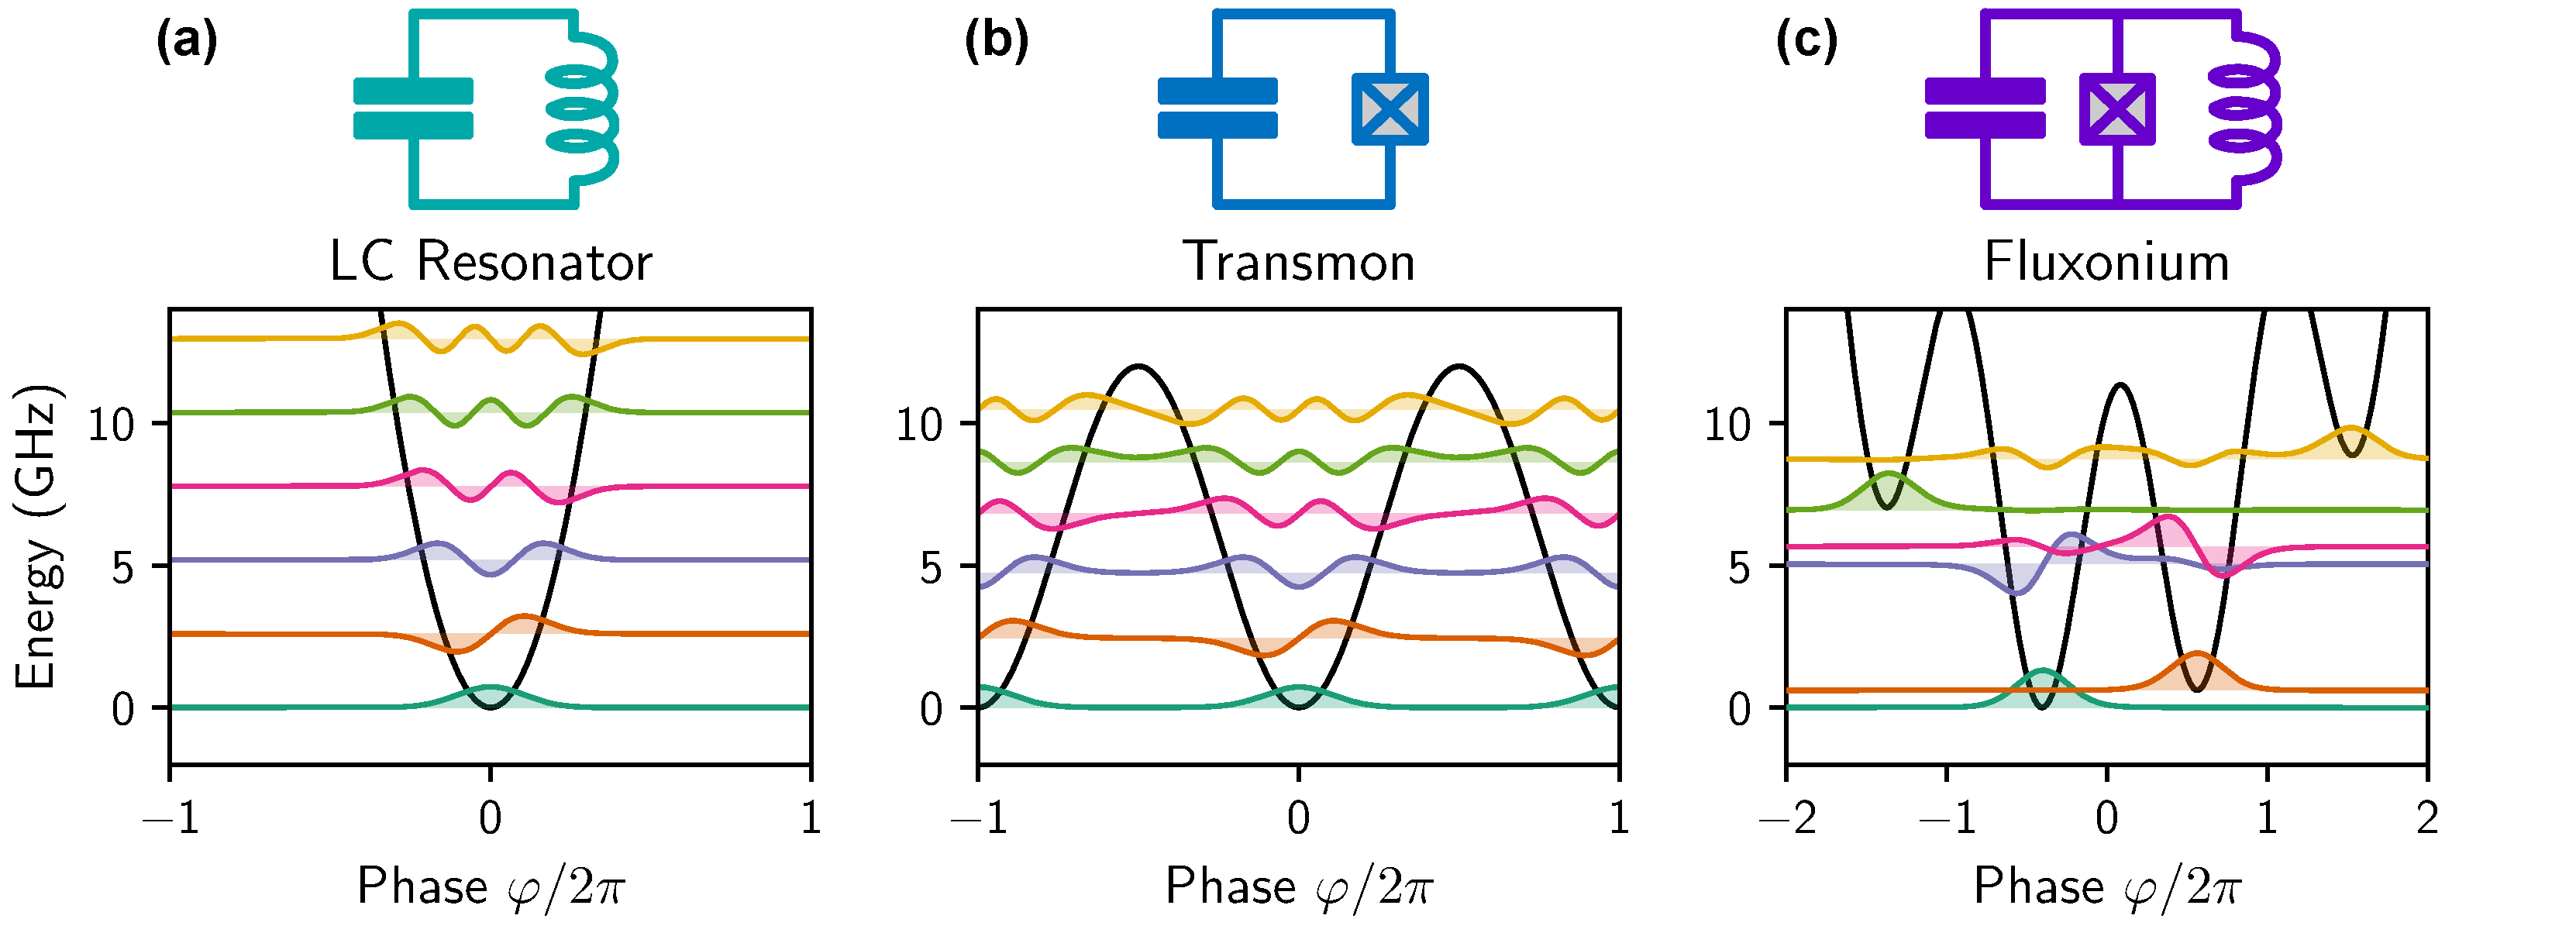
\includegraphics[width=\linewidth]{Figures/3/Circuit_QED_Overview.pdf}
    \caption{In this chapter, we will review three common superconducting circuits: the LC resonator, the transmon qubit, and the fluxonium, whose circuit diagrams, wavefunctions, and potential energies (black solid lines) are shown.}
    \label{fig:3_Circuit_QED_Overview}
\end{figure}
\clearpage
% % ------------------------------------------------

% %%%%% Chapter 4: 3D GKP Project %%%%%%
\chapter{Fluxonium in a 3D Cavity: Experiments\label{ch:4_3DGKP}}
In this chapter, we will introduce our first experimental implementation using fluxonium as the control qubit for an oscillator. In this experiment, we integrated a heavy fluxonium chip into a 3D superconducting cavity resonator architecture. We will start by introducing the basic idea behind the experiment in Sec. \ref{sec:4_3D_Experiment_Design_Theory}, followed by a discussion of the hardware we used to implement it in \ref{sec:4_Hardware_and_Setup}. We will then present an assortment of experimental results that we obtained with this system in Secs. \ref{sec:4_Resonator_and_Two_Tone}-\ref{sec:4_StorageCoherenceProblems}, highlighting both our successes as well as the many challenges we encountered.  



\section{Experimental Design and Theory \label{sec:4_3D_Experiment_Design_Theory}}
The basic model that we considered for this experiment is that of a fluxonium dispersively coupled to a storage resonator, as was discussed in Sec. \ref{sec:3_Circuit_QED_with_Fluxonium}. Here, we specifically started from 
\begin{equation}
    \hat{H} = \omega_s \hat{a}^\dagger \hat{a} + \Big[4E_C \hat{n}^2 + \frac{1}{2}\hat{\varphi}^2 - E_J\cos(\hat{\varphi}+\varphi_{\rm ext})\Big] + g\hat{\varphi}(\hat{a} + \hat{a}^\dagger)
    \label{eq:4_3DGKP_StorageQubit_H}
\end{equation}
with the storage-fluxonium interaction described via an inductive coupling term as shown above. The theory in Sec. \ref{sec:3_Circuit_QED_with_Fluxonium} allows us to get an effective dispersive model from Eq. \eqref{eq:4_3DGKP_StorageQubit_H}. 

The main goal of this experiment was to eventually demonstrate bosonic QEC with the GKP code which, as we saw in Ch. \ref{ch:2_QEC} and Ch. \ref{ch:3_cQED}, requires an effective dispersive interaction $\chi\hat{a}^\dagger\hat{a}\sigmaz/2$ to realize conditional displacements operations [see e.g., the ECD scheme from Sec. \ref{sec:2_ECD}]. We thus wish to engineer a large dispersive shift $\chi = \chi(\varphi_{\rm ext})$ which ideally can also be tuned with flux to toggle the interaction on and off. The reason for this is that the SBS protocol for open-loop GKP error correction requires a qubit reset in between rounds of stabilization operations. During this stage, we would like to be able to reset the qubit state to $\ket{g}$ without impacting the quantum information stored in the resonator. If the $\chi$ is large, then the variable time $\tau$ over which the qubit is reset will result in dephasing of the storage at a rate $\sim \chi\tau/2$ due to the dispersive coupling \cite{sivak2023gkp-expt, nordquantique2023gkp-expt}. Luckily, the rich structure of the fluxonium allows us to engineer a flux-tunable dispersive shift $\chi(\varphi_{\rm ext})$ that crosses through zero at a given flux operating point. 
\begin{figure}[h]
    \centering
    \includegraphics[width=0.85\linewidth]{Figures/4/SBS_Control_and_Reset.pdf}
    \caption[Control and reset phases of the open-loop GKP error correction.]{GKP open-loop error correction consists of two sections: control (green) and reset (red). For control, we want large $\chi$ to get fast conditional displacements. For reset, we want $\chi = 0$ to minimize backaction on the storage mode.}
    \label{fig:4_SBS_Control_and_Reset}
\end{figure}

In addition to having a large dynamic-range for the dispersive shift over some given set of external fluxes, we also wish to minimize the Kerr nonlinearities $K_g$ and $K_e$ since these terms are detrimental for bosonic QEC. Finally, we wish to be in the \textit{heavy-regime} of the fluxonium with $E_J \gg E_C$ in order to benefit from the bit-flip protection of the heavy fluxonium, which is the main reason that we are using this qubit in the first place. Simultaneously achieving all the conditions above requires us to do a multi-dimensional parameter optimization. We discovered, however, that it is possible to engineer the system to meet these requirements by carefully choosing the storage mode frequency to be \textit{between} the two sets of so-called fluxonium plasmon transitions, which are the transitions from the states $\ket{g}, \ket{e}$ to the higher excited states of the two wells, $\ket{f}$ and $\ket{h}$. At half-flux, the coupling between these plasmon states results in an avoided crossing (i.e., an energy gap), which we can use to engineer the dispersive shift $\chi(\varphi_{\rm ext})$ by placing $\omega_{gf} < \omega_s < \omega_{gh}$ and $\omega_{ef} < \omega_s < \omega_{eh}$. We refer to this condition as  \textbf{bosonic mode threading}, since the storage is 
\textit{threaded} through the gap between the two plasmon states. In our numerical simulations, we found that the bosonic mode threading condition results in $\chi(\varphi_{\rm ext})$ crossing through zero (for $E_J, E_C, E_L$ in the right range), and also minimizes the effective Kerr nonlinearity. By numerically investigating Eq. \eqref{eq:4_3DGKP_StorageQubit_H} using threading as a guideline, we ultimately settled on the parameters $\omega_s/2\pi = 8.907$ GHz, $E_J/h = 8.74$ GHz, $E_C/h = 1.69$ GHz, $E_L/h = 0.5$ GHz, and coupling strength $g/2\pi = 24$ MHz. With these parameters, we get a flux-tunable dispersive shift that can be tuned from -1 to +1 MHz in the flux range of interest, as well as reasonably low Kerr nonlinearities satisfying $K_i/\chi \lesssim 5\times 10^{-3}$ for $i \in \{g, e\}$ [cf. Fig \ref{fig:4_3D_GKP_Theory_ChiKerr}]. 

\begin{figure}[h]
    \centering
    \includegraphics[width=0.93\linewidth]{Figures/4/3D_GKP_Theory_Spectrum.pdf}
    \caption[Simulated energy spectrum obtained from numerical diagonalization of the fluxonium Hamiltonian for 3D-GKP experiment.]{Energy spectrum obtained from numerical diagonalization of the fluxonium Hamiltonian with $E_J/h = 8.74$ GHz, $E_C/h = 1.69$ GHz, $E_L/h = 0.5$ GHz. The transitions $\ket{g/e}\to\ket{n}$ are colored by their phase matrix elements. We overlay the storage frequency $\omega_s/2\pi = 8.907$ GHz and see that it is \textit{threaded} between the two sets of plasmon transitions.}
    \label{fig:4_3D_GKP_Theory_Spectrum}
\end{figure}
\begin{figure}[h]
    \centering
    \includegraphics[width=0.93\linewidth]{Figures/4/3D_GKP_Theory_ChiKerr.pdf}
    \caption[Simulated dispersive shift and Kerr nonlinearities obtained from numerical diagonalization of the resonator-fluxonium system using the parameters of the 3D-GKP experiment.]{Left: Storage dispersive shift $\chi(\varphi_{\rm ext})$ obtained from numerical diagonalization of Eq. \eqref{eq:4_3DGKP_StorageQubit_H}. We see $\chi$ tunes with flux and crosses through zero at $\Phi_{\rm ext} \approx 0.483\Phi_0$, which is where we would perform reset. Right: Storage Kerr nonlinearities $K_g$ and $K_e$ when qubit is in $\ket{g}$/$\ket{e}$ respectively. We also plot $K = [K_g+K_e]/2$ and $dK = [K_g-K_e]/2$.}
    \label{fig:4_3D_GKP_Theory_ChiKerr}
\end{figure}

\clearpage
\section{Hardware and Setup\label{sec:4_Hardware_and_Setup}}

\subsection{3D Cavity-Fluxonium Architecture \label{sec:4_3D_Cavity_Resonators}}
To implement the proposed experiment above, we designed a package consisting of three superconducting 3D post cavities fabricated from high-purity (``5N5'') aluminium, as well as a PCB and interconnect module on which we mounted two fluxonium qubit chips. We refer to the three cavity resonators as ``A'', ``B'', and ``C'' from left to right; cavity B serves as the storage resonator, while cavities A and C serve as readout resonators for the qubits [see Fig. \ref{fig:4-3DGKP-schematic-1}(b)]. We designed the package in this way to be able to screen multiple fluxonium devices per cooldown. The chips themselves were fabricated at MIT Lincoln Laboratory out of aluminium on an 8" Si wafer, while the cavity and housing were fabricated at MIT, and then later cleaned and etched in the MIT.nano cleanroom. For additional details about the cavity fabrication, see Appendix \ref{ch:AppB}. A schematic diagram summarizing the fluxonium chip design is shown in Fig. \ref{fig:4-3DGKP-schematic-2} below.

\begin{figure}[h]
    \centering
    \includegraphics[width=0.95\linewidth]{Figures/4/3DGKP-Schematic-1.pdf}
    \caption[Hardware overview of 3D cavity architecture, showing both the assembled and disassembled packages.]{\textbf{(a)} Assembled 3D cavity-fluxonium package. \textbf{(b)} Disassembled view showing qubit chips glued to the interconnect module and wirebonded to a PCB for signal delivery. The chips are then inserted into the chip tunnels and screwed tight with an indium seal to assemble the package. Cavities are labelled A, B, C from left to right; cavity B serves as the storage. All three cavities are driven via SMA pins (gold); the drive port is weakly coupled for the storage resonator to minimize loss and strongly coupled for the readout resonators. Inset: inner structure of the three post cavities. Each stub forms a $\lambda/4$ resonator.}
    \label{fig:4-3DGKP-schematic-1}
\end{figure}

We will refer to the specific cavity device shown in Fig. \ref{fig:4-3DGKP-schematic-1} as the ``Mark II'' cavity. Our first attempt at fabricating a 3D cavity resonator (the ``Mark I'') had low resonator lifetimes due to an unsuccessful etch process (etching is required in order to realize high quality-factors in a 3D cavity; see App. \ref{ch:AppB}). All of the fluxonium experiments in this thesis were performed using the Mark II. Before inserting the qubit, however, we performed cryogenic measurements of the bare cavities in order to characterize their coherence. We measured the lifetime of the storage resonator to be $T_1 \approx 765$ $\mu$s, which we extracted from a fit of the resonator response to a reflection measurement using a Vector Network Analyzer (VNA). For more details about such resonator measurements, see App. \ref{ch:AppA}. Later, after optimizing our etch process, we also fabricated a ``Mark III'' cavity; while we did not use it for any of the experimental results shown in this chapter, the Mark III was helpful to have for later debugging. The bare storage lifetime in \textit{this} cavity was found to be in excess of $T_1 \approx 3$ ms. 

\begin{figure}[h]
    \centering
    \includegraphics[width=\linewidth]{Figures/4/3DGKP-Schematic-2.pdf}
    \caption[Schematic of the fluxonium chip used in the 3D cavity architecture.]{Schematic of qubit chip in the 3D cavity architecture. \textbf{(a,b)} Fluxonium design showing capacitor pads (purple) and a shared superinductance with an auxiliary \textit{antenna} mode (pink). The antenna pads are then extended to the chip edge to implement coupling to the post cavities; the fluxonium-resonator couplings are thus mediated via the antenna. \textbf{(c)} The fluxonium is flux biased using an on-chip wideband flux line capable of delivering both radio-frequency (RF) and DC signals; the flux line terminates in a loop (cf. panel b) and the current returns via the ground plane (teal blue in panel c, representing aluminium metallization on the chip). \textbf{(d)} Chip integrated in 3D cavity showing the chip edge partially extending into both the storage and readout cavities (teal and lilac posts, respectively) to implement couplings. The schematic in panel d focuses on a single storage-qubit-readout subsystem of the package; the full system includes another qubit and readout (cf. Fig \ref{fig:4-3DGKP-schematic-1})}
    \label{fig:4-3DGKP-schematic-2}
\end{figure}

%\todo{Fitting to get pin lengths.}


\subsection{Cryogenic Setup}

The experiments were performed using a Leiden CF-CS81 dilution refrigerator operated at base temperatures of 8-10 mK. The fridge consists of five temperature stages\footnote{The fridge temperature is primarily tracked using three 1 k$\Omega$ platinum (PT-1000) thermometers at the 50K, 3K, and MXC plates. The 3K plate also has a 10 k$\Omega$ RuO$_2$ sensor, while the MXC has additional resistive and CMN magnetic susceptibility thermometers. We note that the fridge has high-power heaters at the 50K and 3K stages for fast warm-ups, and also features a liquid nitrogen pre-cooling circuit for fast cooldowns.} as shown in Fig. \ref{fig:4-fridge-wiring}, as well as seven shielding cans that each thermalize to a different temperature stage (not pictured). Specifically, we have two vacuum cans thermalized to room temperature and 1K respectively, and three other cans for additional electromagnetic shielding. We mount devices on a ``cold finger'' that is thermalized to the mixing chamber (MXC) and encapsulated in a mu-metal shield to protect against infrared radiation and stray magnetic fields. A timelapse video of the process to install these various shields can be found \href{https://youtu.be/KkvUc9Aw77s?t=829}{\textbf{here}}. 

\begin{figure}[h]
    \centering
    \includegraphics[width=0.9\linewidth]{Figures/4/Fridge-Wiring.pdf}
    \caption[Internal structure of the Leiden CF-450 dilution refrigerator used for the experiments in this thesis.]{Left: Internal structure of the Leiden CF-450 dilution refrigerator used for the experiments in this thesis. The fridge consists of several plates/stages each thermalized to successively colder temperatures. Right: Devices are mounted onto a ``cold finger'' that is thermalized to the mixing chamber (MXC) plate at 10 mK.}
    \label{fig:4-fridge-wiring}
\end{figure}
\clearpage

The specific experiments presented in this thesis used both DC and radio-frequency (RF) microwave lines to deliver signals to the 3D cavity and fluxonium package. We used three microwave ``drive'' lines for the two fluxonium qubits and the storage resonator, as well as two DC twisted pair connections to provide static flux biasing for the two qubits. The qubit RF and DC signals were first individually filtered and then combined at the mixing chamber through an RF choke. We filtered the DC component using a Mini-Circuits VLFX-300+ low-pass filter, while the RF component was filtered via a K\&L Microwave 12 GHz low-pass filter. This configuration allowed us to probe the higher level transitions of the fluxonium via two-tone spectroscopy through the qubit drive line. 

To attenuate thermal noise coming from the room temperature setup, several attenuators were placed along each of the input microwave lines: a total of 50 dB for the ``drive'' lines and 70 dB for the ``readout'' line. The readout setup had several salient features worth noting: firstly, we used just a single microwave line connected to the two readout cavities via microwave switch; by setting the switch configuration, we selected which of the cavities to measure. Secondly, we used circulators to measure the cavity resonances in reflection. Finally, the reflected output readout signal was pre-amplified using a Josephson travelling wave parametric amplifier (TWPA) at the MXC stage, before being further amplified by a low-noise high-electron-mobility transistor (HEMT) amplifier at 3K, and then a room temperature MITEQ amplifier. The full wiring schematic for this setup is shown below in Fig. \ref{fig:4-microwave-wiring-diagram}. 

At room temperature, pulse waveforms for the various elements were generated using an OPX+ controller from Quantum Machines. For the storage drive, we used an Agilent PSG Signal Generator (E8267D) from Keysight to supply an RF signal which was then combined with the intermediate-frequency (IF) signal from the OPX using the PSG's internal wide-bandwidth IQ mixer. The qubit drive was produced similarly, using a separate Agilent PSG Signal Generator. When performing low-frequency two-tone spectroscopy of the fluxonium $g$--$e$ transition, however, we bypassed the Agilent and instead used baseband signals in the 0-350 MHz range directly from the OPX. Finally, the readout resonator IF signals were generated via the OPX and then passed into a Rohde and Schwarz SGS100A SGMA RF source for upconversion using an internal IQ mixer. The local oscillator (LO) reference signal used for IQ modulation was also passed on to a separate external IQ mixer to demodulate the readout RF output signal coming out of the fridge. The demodulated intermediate-frequency I and Q components were then digitized and processed using the FPGA within the OPX. All microwave signal generators were frequency-locked via a common 10 MHz rubidium clock. 

The DC signals used for static flux biasing were generated via a Yokogawa GS200 Voltage/Current source operated in ``Voltage'' mode; this was then sent into the Qdevil breakout board and then into the fridge via a Fisher cable. Once in the fridge, the signal lines were passed through a resistive DC low-pass filter before terminating in a twisted pair connection. When operating a Yokogawa (or ``Yoko'') in Voltage mode, the DC signal is typically routed through a 1-10 k$\Omega$ resistor to produce an associated current; anecdotally around our lab, this has also been reported to help reduce flux noise from DC lines. However, in the experiments reported below, we mostly chose not to do this and instead used only the bare resistance of the DC line when connected to the fluxonium device, which we measured to be 152.5 $\Omega$ using a multimeter when the fridge was cold. This allowed us to generate a larger current for a given voltage. As we discuss in Sec. \ref{sec:4_Time_Domain}, we later also measured the flux noise amplitude of the qubit when using the ``Current'' mode of the Yoko and found negligible differences in the results. % \todo: check DC low-pass filter

\begin{figure}[ht]
    \centering
    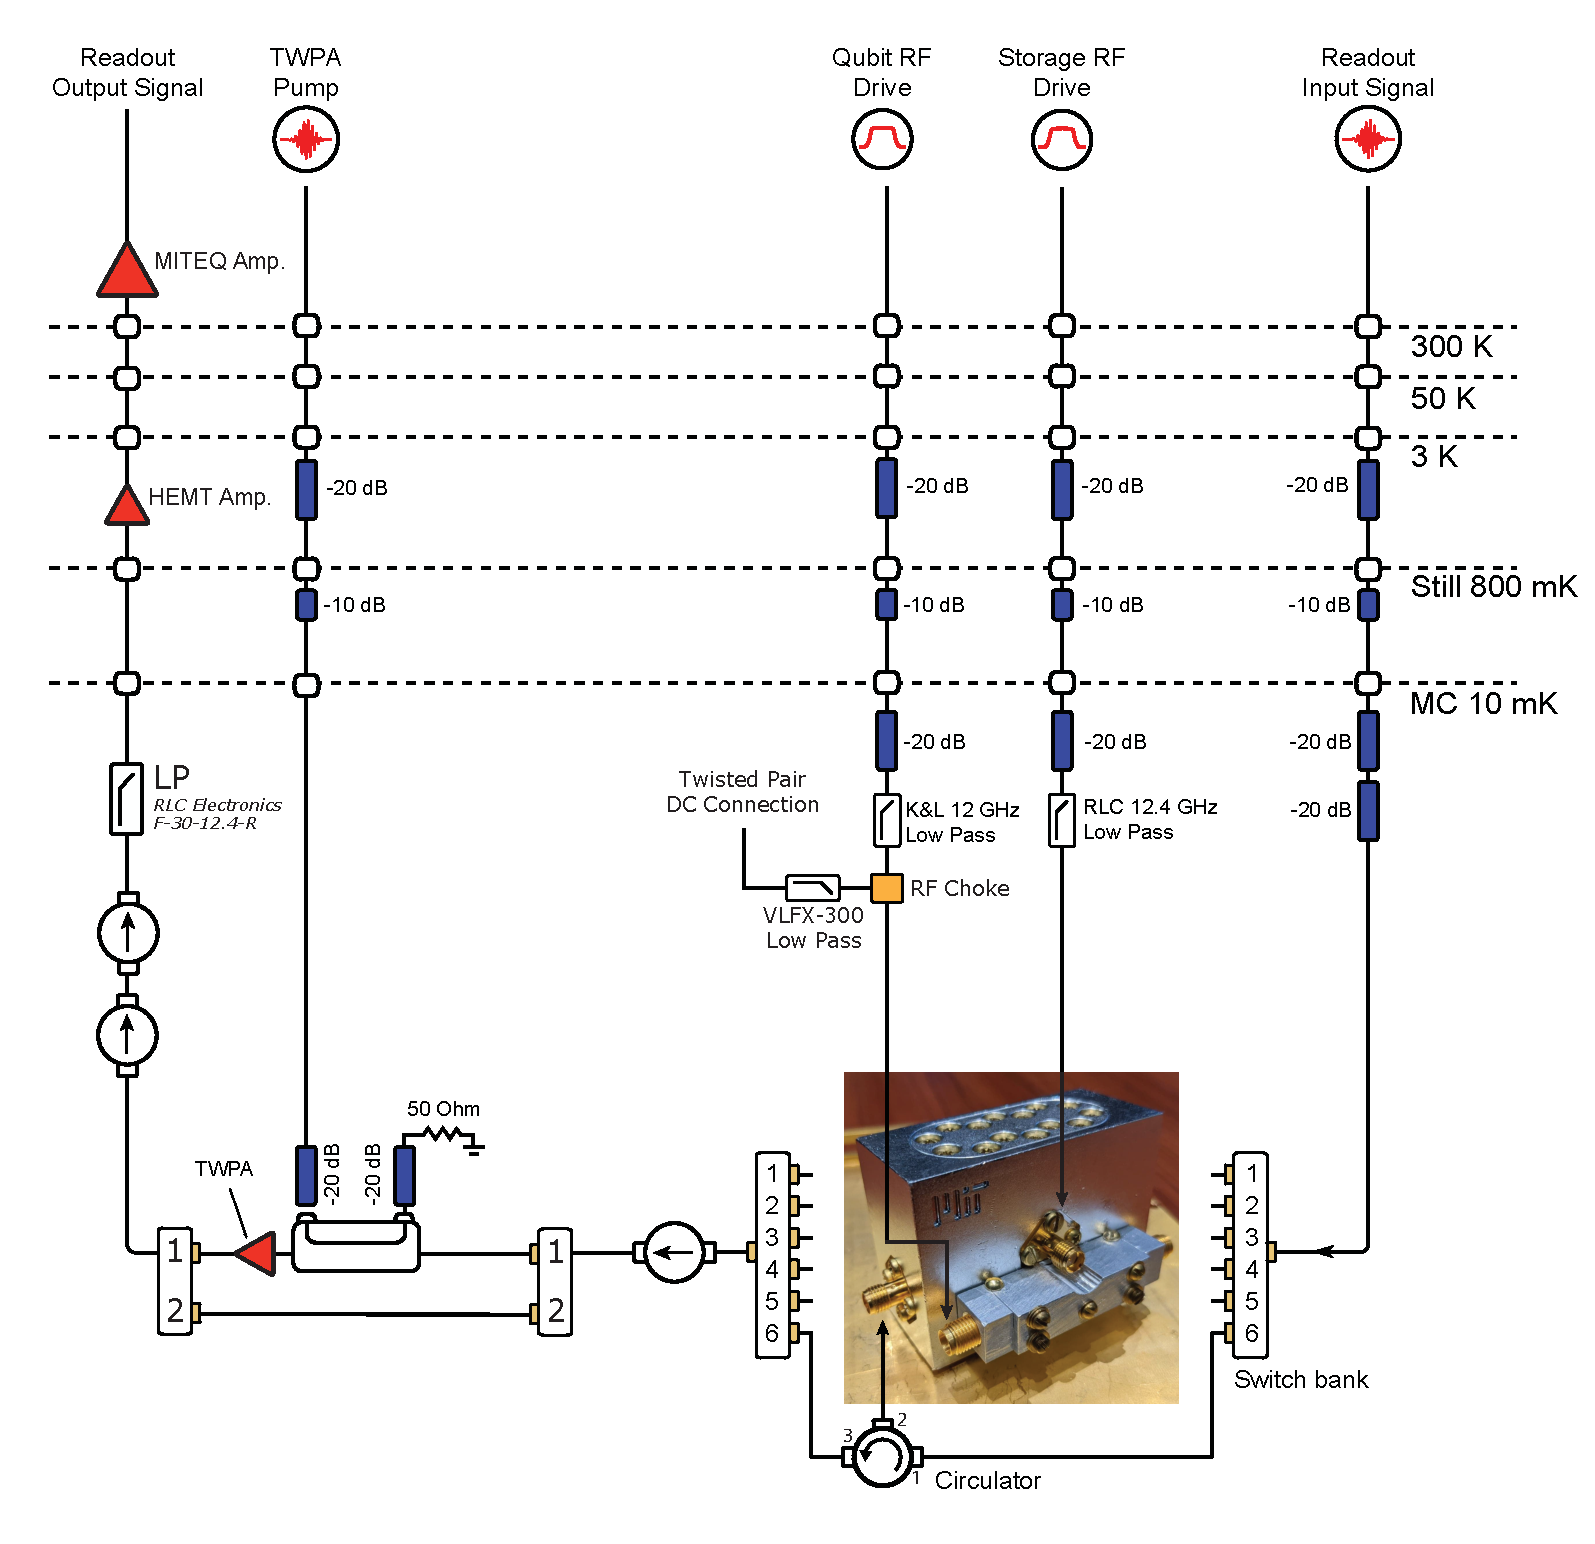
\includegraphics[width=\linewidth]{Figures/4/Microwave-Wiring-Diagram.pdf}
    \caption[Microwave wiring diagram for the experiment.]{Wiring diagram for the experiment consisting of a readout chain set up in a reflection configuration and RF drives for the fluxonium qubit and storage resonator. We combine the qubit RF signal with a DC bias at the mixing chamber using an RF choke.}
    \label{fig:4-microwave-wiring-diagram}
\end{figure}


\clearpage
\section{Resonator and Two-Tone Spectroscopy\label{sec:4_Resonator_and_Two_Tone}}

In this section, we will present experimental results from our first 3D cavity-fluxonium device with a GKP1 fluxonium chip in our Mark II cavity. We begin with a spectroscopic characterization of the readout resonator and qubit here, followed by time-domain measurements of the qubit in Sec. \ref{sec:4_Time_Domain}, and finally discuss storage resonator measurements in Secs. \ref{sec:4_StorageChi} and \ref{sec:4_StorageCoherenceProblems}. Unless stated otherwise, all data in the upcoming sections was taken using readout cavity A and its associated fluxonium chip. We therefore restrict our focus to the subsystem of the Mark II cavity-fluxonium package comprised of cavity A (readout resonator), fluxonium A (qubit), and cavity B (storage resonator).

\subsection{Resonator Spectroscopy}
In most circuit QED experiments, the readout resonator forms a crucial gateway through an experimenter probes the system of interest. To this end, the first measurement step we took after cooling down our device was to locate the readout resonator via spectroscopy. As discussed in Sec. \ref{sec:4_3D_Cavity_Resonators}, the readout pin length was chosen here to be overcoupled, with a target coupling rate of $\kappa_c/2\pi \approx 10$ MHz. We were thus able to locate the cavity resonance fairly easily using the VNA and later via pulsed resonator spectroscopy on the OPX with a 10 $\mu$s pulse [see Fig. \ref{fig:4_resonator_spectroscopy}(a)].
\begin{figure}[h]
    \centering
    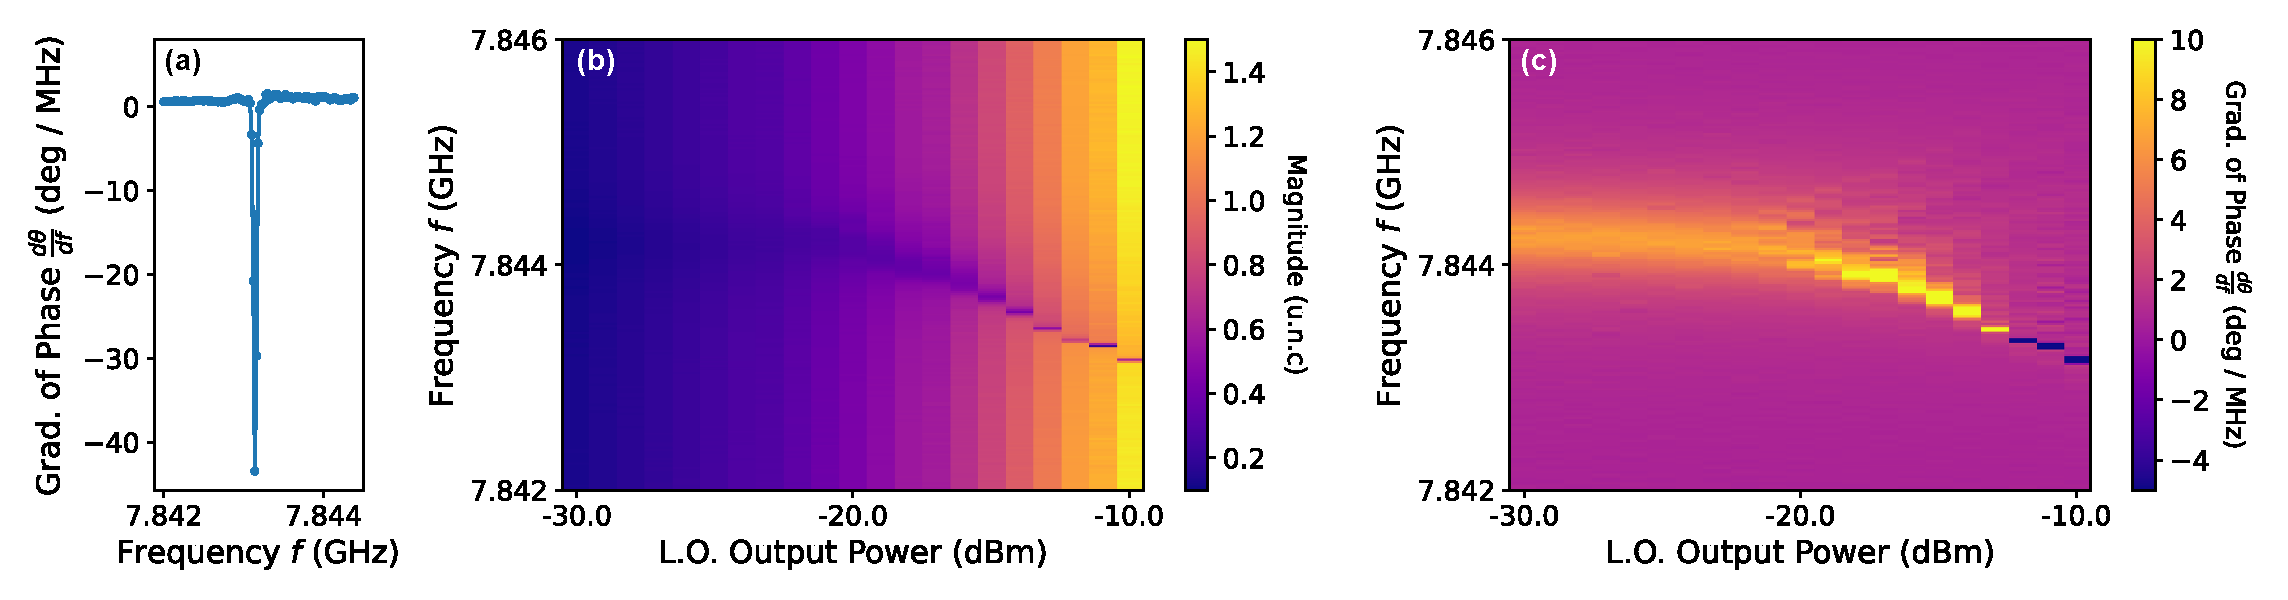
\includegraphics[width=\linewidth]{Figures/4/resonator_spectroscopy.pdf}
    \caption[Resonator spectroscopy experiments showing a single resonator spectrum and a sweep vs. drive power.]{\textbf{(a)} Readout cavity resonance measured using a time-domain resonator spectroscopy sequence. We plot the gradient of the phase $\theta$ of the reflected signal. \textbf{(b,c)} Sweep of resonator spectroscopy vs. drive power; here we plot both the magnitude and phase.}
    \label{fig:4_resonator_spectroscopy}
\end{figure}

We next repeated pulsed resonator spectroscopy as a function of the input power of the resonator tone to realize a so-called ``punchout'' measurement [Fig. \ref{fig:4_resonator_spectroscopy}(b-c)]. In the data, we observe the resonator ``punching'' out, i.e., its frequency shifting downwards towards its bare value as we increase the drive power as it decouples from the nonlinear degrees of freedom in the system (e.g., the qubit or antenna mode here). Punchout is typically used as a way to check whether a qubit is present, since the nonlinearity of the qubit directly results in a nonlinear response in the resonator. For a practical explanation of this, I refer interested readers to Ref. \cite{naghiloo2019introduction} which also gives a step-by-step experimentalist's introduction to qubit measurements in circuit QED. 

Due to its coupling to the fluxonium qubit, we also expect the resonator to inherit some flux dependence in addition to nonlinearity. Therefore, after verifying that the resonator frequency changes with power, we next performed resonator spectroscopy vs. the applied external flux bias on the qubit [see Fig. \ref{fig:4_resonator_spectroscopy_vs_flux}]. We set the bias using the room temperature Yokogawa source to set voltage (which induced a current through the DC line, and in turn generated an applied flux through the fluxonium loop). After setting each bias voltage, we waited for 0.1s for the flux to settle and then performed resonator spectroscopy.  

\begin{figure}[h]
    \centering
    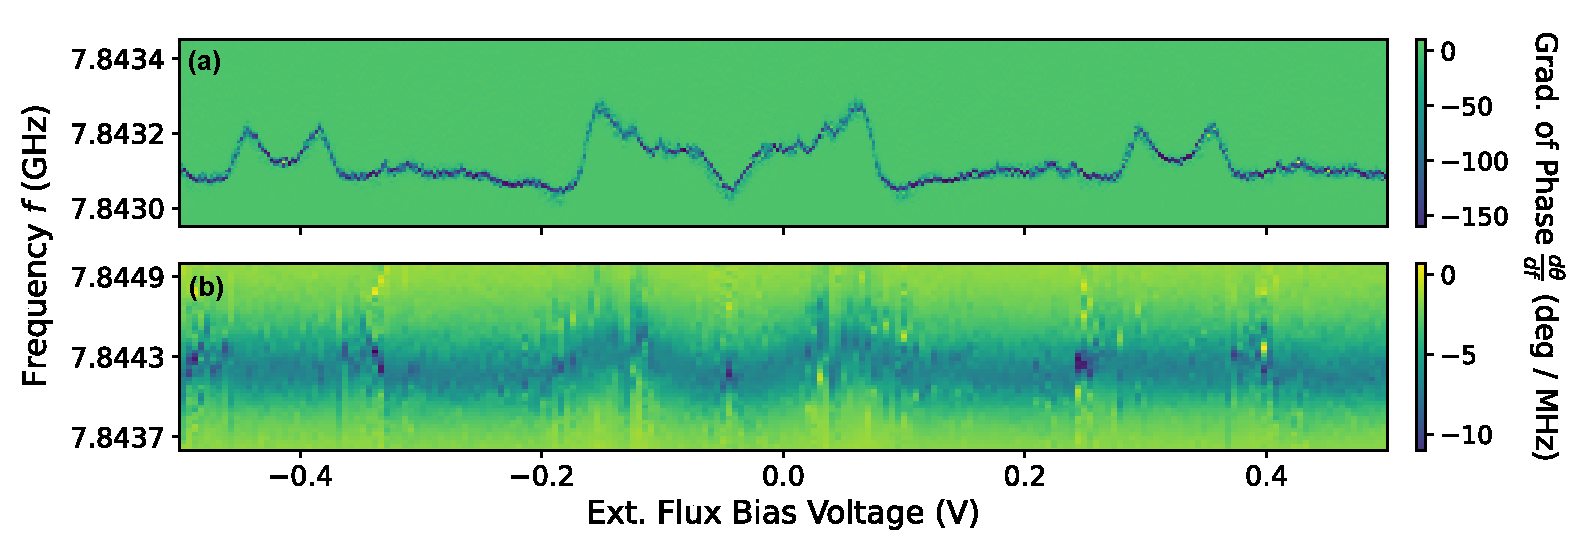
\includegraphics[width=\linewidth]{Figures/4/resonator_spectroscopy_vs_flux.pdf}
    \caption[Resonator spectroscopy vs. external applied flux on the fluxonium qubit.]{Resonator spectroscopy vs. external bias voltage on the qubit. The top panel shows high-power data with an LO output power [cf. Fig. \ref{fig:4_resonator_spectroscopy}] of -10 dBm, while bottom panel shows lower-power data taken at -30 dBm. We see the resonator spectrum is indeed periodic with the bias voltage.}
\label{fig:4_resonator_spectroscopy_vs_flux}
\end{figure}

We see that the the resonator frequency indeed varies periodically with the bias voltage. From the periodicity of the spectrum, we found (and later corroborated via qubit two-tone spectroscopy measurements) that a flux quantum in this device corresponds to 4.872 mA, realized in this configuration via a voltage of about 0.743 V applied over the line resistance of 152.5 $\Omega$. The resonator spectrum is expected to be symmetric about both zero external flux ($\Phi_{\rm ext} = 0$) and ``half-flux'' ($\Phi_{\rm ext} = \Phi_0/2$), and we can observe two symmetry points above --- one at $V_b \approx -0.045$ V, and other at both $V_b \approx 0.326$ V and $V_b \approx -0.414$ V. From the averaged data in Fig. \ref{fig:4_resonator_spectroscopy_vs_flux} alone, it is rather difficult to identify which of these symmetry points corresponds to ``half-flux''. However, we can make this identification by instead working with single-shot data, i.e., not directly averaging across shots on the OPX during readout. At $\Phi_{\rm ext} = 0$, the fluxonium has a single ground state $\ket{g}$ that the qubit relaxes to in thermal equilibrium. Thus the dispersive readout will result in a \textit{single} ``I-Q blob'' in the demodulated signal. However, at $\Phi_{\rm ext} = \Phi_0/2$, both the ground and excited states will be thermally occupied in equilibrium due to the low-frequency nature of the qubit \cite{manenti2023quantum}, and thus we expect to see two ``blobs'' in the I-Q plane corresponding to the qubit initial state being in either $\ket{g}$ or $\ket{e}$. When we set the Yoko voltage to $V_b = -0.04465$ V, the single-shot data [cf. Fig \ref{fig:4_single_shots}] reveals two IQ ``blobs'' in the histogram, confirming that this bias point is, in fact, the half-flux sweet spot. (By association, the other symmetry points correspond to \textit{integer} flux quanta). Using this calibration of the flux axis, we can map between the bias voltage and the applied external flux $\Phi_{\rm ext}$ in all subsequent measurements. 

\begin{figure}[h]
    \centering
    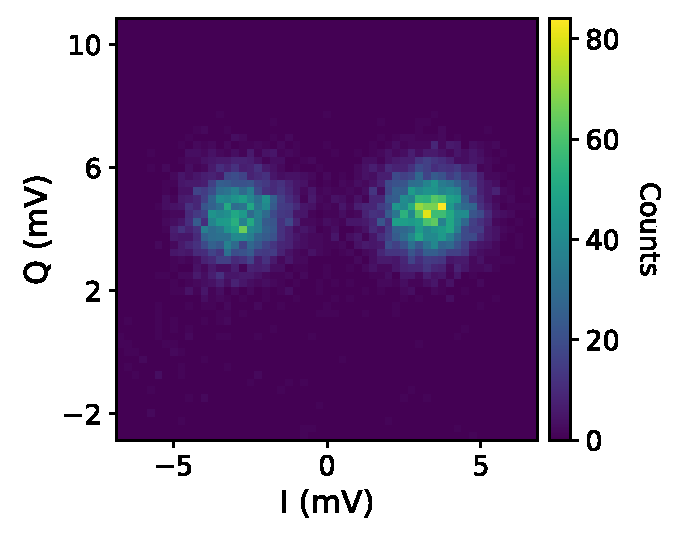
\includegraphics[width=0.51\linewidth]{Figures/4/single_shots.pdf}
    \caption[Readout I-Q histogram for a fluxonium parked at half-flux.]{Histogram of 10,000 digitized single-shot readout measurements, plotted in the I-Q plane. The two ``blobs'' correspond to the two qubit states $\ket{g}$ and $\ket{e}$ that will both be populated in equilibrium when the fluxonium is parked near the half-flux sweet spot.}
\label{fig:4_single_shots}
\end{figure}


\newpage
\subsection{Two-Tone Spectroscopy}
After characterizing the resonator, our next step was \textit{two-tone spectroscopy} (also called qubit spectroscopy). Here, the two ``tones'' in question are (i) a qubit drive tone to probe transitions of the fluxonium, followed by (ii) a resonant readout tone. Practically, we can understand a two-tone spectroscopy experiment as follows by considering the dispersive Hamiltonian \cite{zhu2013cQEDfluxonium}:
\begin{equation}
    \hat{H} = \sum_k \tilde{\omega}_k \op{k}{k} + \bigg(\omega_r^0 + \sum_k \chi_k \op{k}{k}\bigg) \hat{a}^\dagger\hat{a}
\end{equation}
We have Lamb-shifted qubit energies $\tilde{\omega}_k$ and eigenstates $\ket{k}$, as well as a resonator whose effective frequency $\tilde{\omega}_r$ (term in parentheses) depends on the qubit state. For the sake of illustration, let's briefly work near zero flux so that only the ground state $\ket{g}$ is initially populated in thermal equilibrium. The basic idea of the experiment is to play a weak continuous spectroscopy (or ``\textit{saturation}'') tone on the qubit. As we sweep the frequency, we will eventually come into resonance with a qubit transition, e.g., $\tilde{\omega}_{gl} = \tilde{\omega}_{l} - \tilde{\omega}_{g}$ between $\ket{g}$ and some other state $\ket{l}$. When this happens, the resonant tone has the effect of driving Rabi oscillations between the states $\ket{g} \leftrightarrow \ket{l}$; furthermore, over many multiples of the coherence time, the qubit state will also change due to decoherence processes (i.e., $T_1$ relaxation and heating, as well as dephasing). The qubit will thus be left in a non-equilibrium steady state $\hat{\rho}$ with occupation probabilities $p_k$. Due to the dispersive interaction, this mixed state in turns leads to an average resonator frequency
\begin{equation}
    \ev{\tilde{\omega}_r}_{\rm final} = \omega_r^0 + \Tr\bigg(\hat{\rho} \sum_k \chi_k \op{k}{k}\bigg) = \omega_r^0 + \sum_k p_k \chi_k
\end{equation}
that is different from the initial one: $\ev{\tilde{\omega}_r}_{\rm init} = \omega_r^0 + \chi_g$. Using a resonator measurement, we can then detect this change in the resonance frequency (e.g., by measuring the change in signal phase when ``reading out'' at a fixed frequency $\ev{\tilde{\omega}_r}_{\rm init}$), and so map out the qubit transitions. If we now do this as a function of flux, the initial qubit state may also need to be described by a mixed state, e.g. a thermal mixture of $\ket{g}$ and $\ket{e}$ near half-flux; nevertheless, as long as the initial and final mixed states lead to different average resonator frequencies, we will be able to identify that a transition has occurred. 

In experiment, we performed wideband two-tone spectroscopy to map out the higher energy transitions of the fluxonium versus external flux. The full spectrum is shown below in Fig. \ref{fig:4_two_tone_vs_flux_full}; we already see a rich set of features in the data. The qubit transitions have a clear dependence on flux, and are notably symmetric about the two sweet spots at $\Phi_{\rm ext} = 0$ and $\Phi_{\rm ext} = \Phi_0/2$. In panel (b), we overlay a theoretical prediction obtained from numerical diagonalization of the fluxonium Hamiltonian with free parameters $E_C$, $E_J$, and $E_L$. We extract
\begin{equation}
    E_C/h \approx 1.678 \,\, \text{GHz}, \quad  E_J/h \approx 8.987 \,\, \text{GHz}, \quad  E_L/h \approx 0.342 \,\, \text{GHz} 
    \label{eq:4_qubit_parameters_fit}
\end{equation}
as the qubit parameters for this device by fitting to the data. This is within the range that we designed for, and results in a qubit frequency of approximately 94.1 MHz at half-flux. 

At this resolution, there are also certain features that appear to be constant with flux. We can identify these as the various linear modes in the system, e.g. the storage resonator at 8.86 GHz, and the two on-chip antenna modes at 8.60 GHz and 8.46 GHz. Since each of these modes has a dispersive shift to the readout resonator (also shown), we are able to see them in this two-tone measurement just as we do the other qubit transitions\footnote{We can also see some other faint qubit-like transitions near half-flux. We'll comment on these later, as they are actually quite interesting: it turns out that they are two-photon ``parasitic'' qubit-resonator transitions.}. Note that each of these linear modes (including the readout) has \textit{some} flux dispersion if we zoom in close enough. This is important for readout calibration, as typically the readout frequency must be calibrated at each new flux operating point. In the data shown here, we did not do this, and instead used a constant frequency tone at 7.8442 GHz, which was approximately resonant across the entire flux range (cf. low-power data in Fig. \ref{fig:4_resonator_spectroscopy_vs_flux}). While this worked reasonably well, we nonetheless see variations in the readout contrast that could be improved by first redoing resonator spectroscopy at each flux point prior to two-tone, or by creating a lookup table ahead of time. 

From the spectrum, we also clearly see that the storage resonator frequency indeed lies in between the two sets of fluxonium plasmon transitions. This is precisely the condition we wanted to engineer in our system: as a reminder, we refer to it at bosonic mode threading. We highlight the threading condition in a zoomed-in scan below [cf. Fig. \ref{fig:4_two_tone_vs_flux_zoom}]. 

\begin{figure}[t]
    \centering
    \includegraphics[width=0.88\linewidth]{Figures/4/two_tone_vs_flux_full.pdf}
    \caption[Wideband two-tone spectroscopy showing the landscape of transitions in our 3D-cavity package.]{\textbf{(a)} Wideband two-tone spectroscopy showing the landscape of transitions in our 3D-cavity package. \textbf{(b)} Overlaid fitted theoretical predictions based on numerical diagonalization of the fluxonium Hamiltonian with free parameters $E_C$, $E_J$, $E_L$. We plot simulated qubit transitions $\ket{g/e}\to\ket{n}$ in purple/red respectively, as well as approximate frequencies of the various linear modes in the system such as the storage, readout, and antennas (shown as straight lines here). Note, due to unwanted crosstalk, we were able to measure antenna C via readout cavity A. Finally, we also highlight two-photon transitions as thin dashed lines. We will comment on these in more detail in the main text.}
\label{fig:4_two_tone_vs_flux_full}
\end{figure}
\clearpage
\begin{figure}[hp]
    \centering
    \includegraphics[width=0.73\linewidth]{Figures/4/two_tone_vs_flux_zoom.pdf}
    \caption[Zoomed-in two-tone spectroscopy showing bosonic mode threading of the storage resonator frequency between the fluxonium plasmon transitions.]{Zoomed-in two-tone spectroscopy showing bosonic mode threading, with the storage resonator frequency in between the two sets of fluxonium plasmon transitions. Dashed lines from $\ket{g}$ and from $\ket{e}$ show theoretical predictions from numerical diagonalization as before. The storage flux dispersion cannot seen at this resolution.}
\label{fig:4_two_tone_vs_flux_zoom}
\end{figure}

Our next experimental step was low-frequency qubit spectroscopy near half-flux using a direct baseband drive to map out the qubit  $\ket{g}\to\ket{e}$ transition: we show the data below in Fig. \ref{fig:4_qubit_spectroscopy}. Unlike prior measurements, here we used a dual readout post-selection scheme \cite{ding2023FTF} to improve contrast and assign an occupation probability to the qubit. This was crucial to obtain our results, and we will discuss it further in the upcoming section.

\begin{figure}[h]
    \centering
    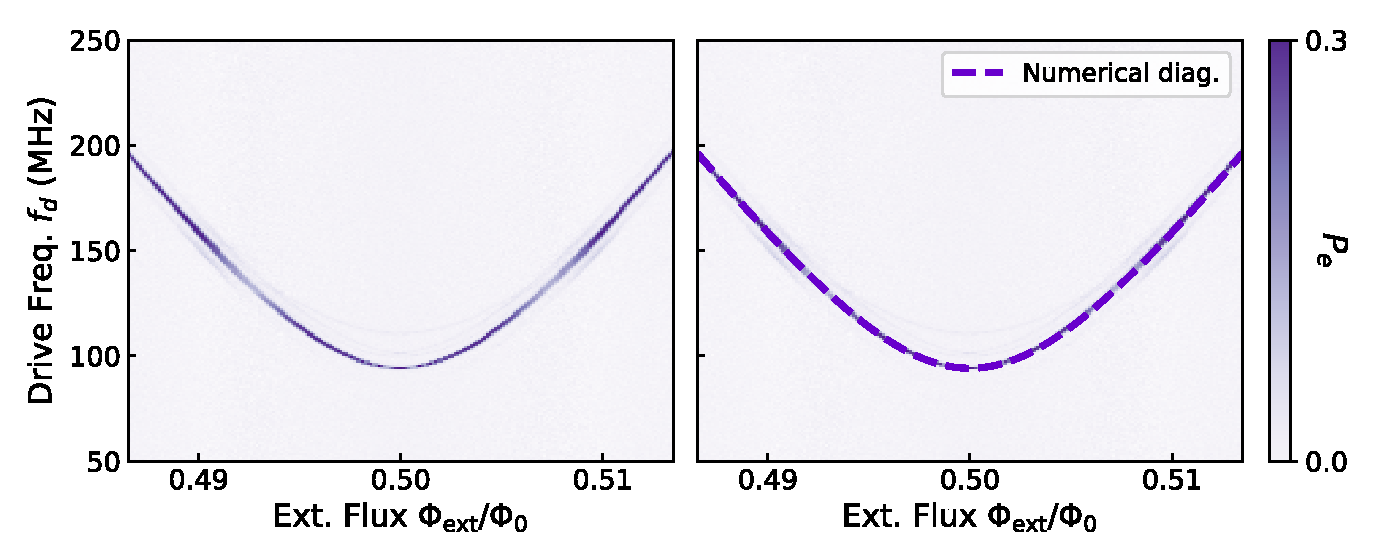
\includegraphics[width=0.88\linewidth]{Figures/4/qubit_spectroscopy.pdf}
    \caption[Baseband two-tone spectroscopy showing the fluxonium qubit $\ket{g}\to\ket{e}$ transition.]{Post-selected baseband two-tone spectroscopy showing the fluxonium $\ket{g}\to\ket{e}$ transition with and without the theoretical fit from numerical diagonalization using the same parameters as before [Eq. \eqref{eq:4_qubit_parameters_fit}]. At half-flux, the qubit frequency is 94.1 MHz.}
\label{fig:4_qubit_spectroscopy}
\end{figure}

\section{Time-Domain Measurements of the Qubit \label{sec:4_Time_Domain}}

\subsection{Post-Selection via Single-Shot Readout}

Near half-flux, the energy of the fluxonium qubit transition $\h\omega_q$ can be much smaller than the ambient temperature $k_BT$ of a typical dilution refrigerator. As a result, the fluxonium in equilibrium will be in a thermal mixture of $\ket{g}$ and $\ket{e}$; we saw this in Fig. \ref{fig:4_single_shots} already. For our specific qubit with frequency $f_q = 94.1$ MHz and assuming an effective temperature of $T = 40$ mK, the excited state population is given by a Boltzman distribution: $p_e = 1 / (e^{+\h\omega_q/k_B T} + 1) \approx 47\%$. For the higher-level (i.e., wideband) two-tone spectroscopy above, this initial thermal distribution was not a problem --- on the contrary, starting from a mixed state is even beneficial, allowing us to see transitions out of both $\ket{g}$ and $\ket{e}$. However, for baseband qubit spectroscopy probing the $\ket{g}\leftrightarrow\ket{e}$ transition, and critically also for time-domain experiments, this ceases to be true. For these measurements, we instead want to be able to discriminate between the two states. In our experiments, the approach we chose to do this was single-shot readout and post-selection. We specifically followed the dual readout scheme discussed in Refs. \cite{ding2023FTF, ding2023thesis} (cf. Fig. \ref{fig:4_postselection} below)\footnote{At this point, I'd also sincerely like to thank Leon Ding for his early guidance with fluxonium experiments!}. Here, the first readout pulse initializes the fluxonium state to either $\ket{g}$ or $\ket{e}$ via projective measurement. We then start the rest of the experimental sequence (e.g., qubit pulses, delays, storage pulses) from a known initial state, and finally conclude with a second readout pulse to record the qubit state. All the time-domain measurements that follow used this post-selected sequence. 

\begin{figure}[h]
    \centering
    \includegraphics[width=0.9\linewidth]{Figures/4/postselection.pdf}
    \caption[Dual-readout post-selection sequence used for time-domain experiments in this thesis.]{Dual readout post-selection. Here, the first readout prepares the qubit in $\ket{g}$ or $\ket{e}$ and the second readout records the final qubit state after performing the experiment sequence. We introduce a short ring-down time $\tau_1$ to allow readout photons to decay after the first readout, and a longer delay $\tau_2$ to let the qubit relax to equilibrium between shots.}
    \label{fig:4_postselection}
\end{figure}

\subsection{Rabi Oscillations and Pi Pulse Calibration}

After having identified the qubit frequency in two-tone spectroscopy, we next turned to time-domain experiments involving coherent manipulation of the qubit state. The first of these was, of course, to demonstrate Rabi oscillations between the $\ket{g}$ and $\ket{e}$ states using a resonant drive. In heavy fluxonium, the $T_1$ protection that arises due to the small charge matrix element also has the effect of making it generically more difficult to drive the associated transitions. As a result, several previous experiments with fluxonium or other low-frequency flux qubits have had to use either non-adiabatic Landau-Zener flux control \cite{oliver2005mach, campbell2020universal, zhang2021universal}, or virtual (Raman) transitions mediated by a higher energy state \cite{earnest2018realization}. Thankfully, we were able to use more conventional microwave-based control via a resonant drive, since our device was not quite so heavy. 

In Fig. \ref{fig:4_rabi}, we show a typical power Rabi measurement, taken with the qubit parked at half-flux. For this data, we specifically used a fixed length ($\tau = 200$ ns) Gaussian pulse whose amplitude we swept to generate Rabi oscillations: this is shown below on the left for a resonant drive. Meanwhile, on the right, we have a characteristic ``chevron'' plot. By finding the point of minimum contrast in the 2D sweep of Rabi frequency and amplitude, we can tune up $\pi$- and $(\pi/2)$-pulses on the qubit. 

\begin{figure}[h]
    \centering
    \includegraphics[width=0.95\linewidth]{Figures/4/rabi.pdf}
    \caption[Power Rabi experiment and Rabi chevrons.]{Left: Power Rabi experiment showing characteristic Rabi oscillations as we sweep the qubit drive amplitude for a resonant pulse. Right: we can sweep the frequency to get a ``chevron'' plot, and then use the minimum contrast point to tune up a $\pi$-pulse.}
    \label{fig:4_rabi}
\end{figure}

In subsequent measurements, we typically tuned up two kinds of $\pi$-pulses: the first was a shorter $\tau = 48$ ns pulse, which we used in most of the time-resolved qubit experiments. The second was a ``selective'' qubit pulse, of length $\tau = 2.4$ $\mu$s, chosen so that the associated spectral bandwidth of the pulse $1/\tau$ was smaller (at least at half-flux) than the dispersive shift $\chi$ between the qubit and storage mode (cf. Sec \ref{sec:4_StorageChi} where we discuss this further). We also later switched from Gaussian to cosine pulses; the latter were easier to work with due to their well-defined end points (zero amplitude at the start and end of the pulse). 

\subsection{Measuring the Fluxonium \texorpdfstring{$T_1$}{T1}\label{sec:4_fluxonium_T1}}

Our next set of experiments involved measuring the $T_1$ relaxation time of the fluxonium. The post-selection sequence we used to realize the measurement consists of two readouts separated by a variable length delay. The first readout initializes the qubit in either $\ket{g}$ or $\ket{e}$, while the second is used to track a change of state. The result is a characteristic $T_1$ relaxation curve showing an exponential decay of the qubit populations with time. We show an example of such a curve in Fig. \ref{fig:4_qubit_T1_vs_flux_single}(a), from which we extract a decay constant $T_1 = 220 \pm 10$ $\mu$s. Panel (b) shows the results of the same experiment now repeated across various external flux biases: we see that the flux-dependence of the qubit $T_1$ is very sharply peaked and symmetric about half-flux, with a maximum value of $T_1 \approx 265$ $\mu$s.

\begin{figure}[h]
    \centering
    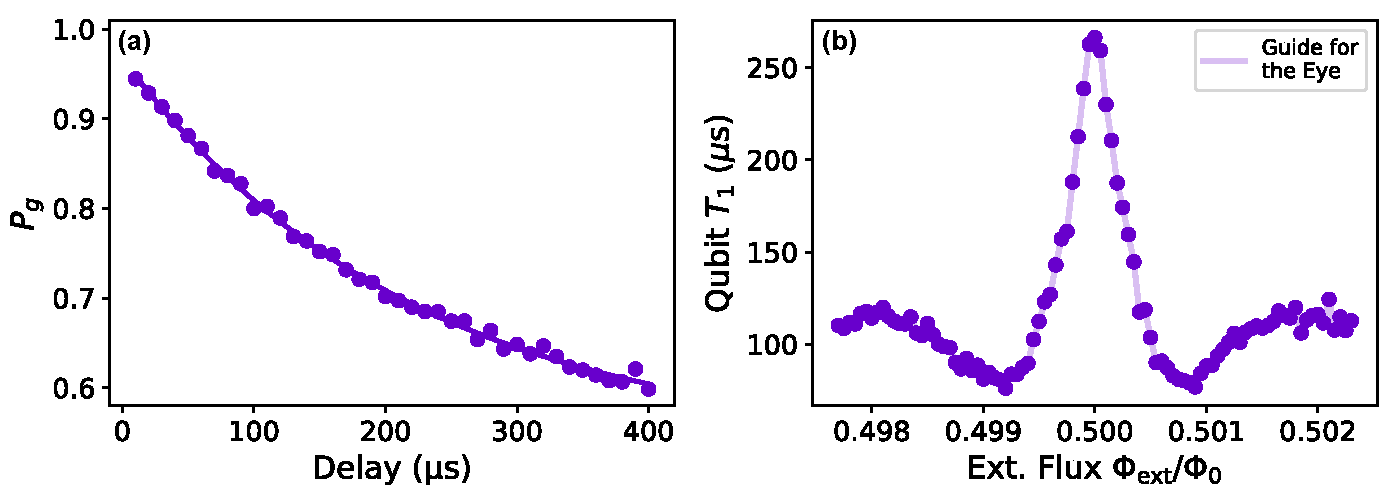
\includegraphics[width=0.95\linewidth]{Figures/4/qubit_T1_vs_flux_single.pdf}
    \caption[Qubit \texorpdfstring{$T_1$}{T1} experiment and sweep of \texorpdfstring{$T_1$}{T1} vs. flux.]{\textbf{(a)} $T_1$ experiment measuring qubit population $P_g$ vs. time. Solid line shows a fit to an exponential decay with an extracted $T_1 = 220 \pm 10$ $\mu$s. \textbf{(b)} Sweep of $T_1$ experiments vs. flux; at each flux, we tune up a $\pi$-pulse and then measure the $T_1$ decay.}
    \label{fig:4_qubit_T1_vs_flux_single}
\end{figure}

The sharply peaked flux-dependence in Panel \ref{fig:4_qubit_T1_vs_flux_single}(b) was one of the first experimental mysteries that we encountered with this device. For the parameters of our fluxonium, and assuming a capacitive (i.e., dielectric) loss model, we naively expected $T_1$ to improve away from half-flux. There are other loss models that would predict $T_1$ degrading away from half-flux (e.g., quasiparticle tunneling); however, we were unable to reproduce the sharp initial drop-off in any numerical simulations at the time of the experiment. [As we discuss below, however, we have since come up with a model that we believe may explain these observations]. 

If we go out even further in flux, we see an even richer structure to the flux-dependence of the fluxonium $T_1$ [see Fig. \ref{fig:4_qubit_T1_vs_flux_spec}]. Away from half-flux, we see a clear drop in $T_1$, followed by an apparent revival around $\Phi_{\rm ext} \approx 0.485\Phi_0$. However, as we move leftwards, we again see further drop-offs in the $T_1$. Although these observations puzzled us for some time, we eventually came to the hypothesis that the drop-offs in $T_1$ may be a form of Purcell decay.

\begin{figure}[h]
    \centering
    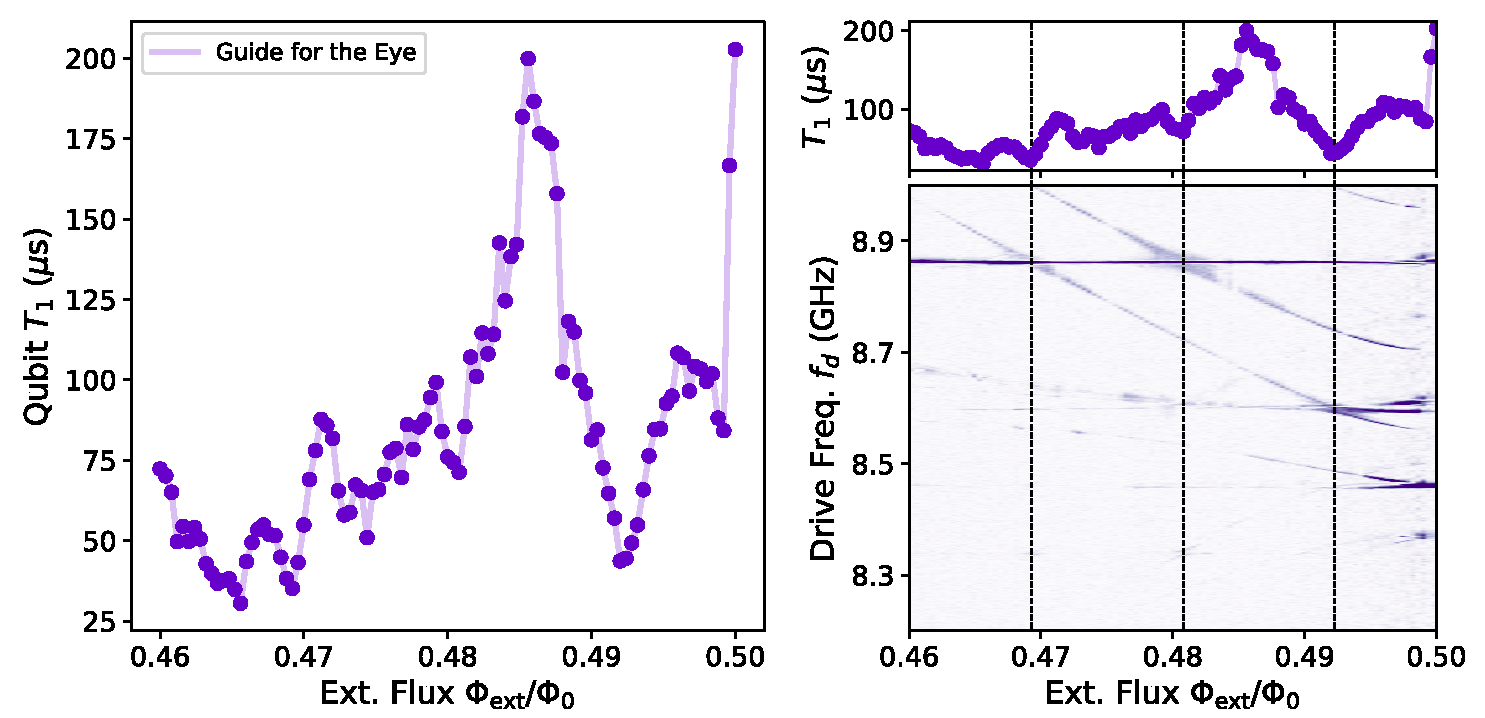
\includegraphics[width=0.95\linewidth]{Figures/4/qubit_T1_vs_flux_spec.pdf}
    \caption[Wider range sweep of qubit \texorpdfstring{$T_1$}{T1} vs. flux.]{Left: Sweep of $T_1$ experiment vs. flux over a wider range of external fluxes. We see rich structure, which we associate with accidential two-photon resonances in the spectrum. Right: we match the locations of the largest qubit $T_1$ drops to two-tone spectroscopy, showing that they coincide with the resonances shown. See main text for details.}
    \label{fig:4_qubit_T1_vs_flux_spec}
\end{figure}

In the right panel of Fig. \ref{fig:4_qubit_T1_vs_flux_spec}, we reproduce the $T_1$ data from the left panel, but also now align it with two-tone spectroscopy data taken earlier. At this resolution, the storage and the two antenna modes are straight lines. On top of these we see certain flux-dependent transitions: it turns out that these are ``two-photon'' transitions! (We showed these in Fig. \ref{fig:4_two_tone_vs_flux_full} as well). Specifically, they correspond to the frequencies of the linear modes \textit{plus} the qubit $\ket{g}\to\ket{e}$ frequency, i.e., they are activated when $\omega_d \approx \omega_{\rm lin} + \omega_{ge}$ where $\omega_{\rm lin}$ can be the frequency of the storage or either antenna. Intuitively, we can understand the drop-offs in qubit $T_1$ occurring when this ``two-photon'' transition is tuned into resonance with one of the \textit{other} linear modes. For example, at $\Phi_{\rm ext} \approx 0.48\Phi_0$, we have $\omega_{\rm C} + \omega_{ge} \approx \omega_{s}$, and at $\Phi_{\rm ext} \approx 0.47\Phi_0$, we have $\omega_{\rm A} + \omega_{ge} \approx \omega_{s}$. In both cases, the resulting resonance leads to a direct Purcell-type decay of the qubit. We have since been able to reproduce this behavior using numerical Purcell simulations, including the initial drop-off at half-flux shown in Fig. \ref{fig:4_qubit_T1_vs_flux_single}; although the latter does not correspond to a direct resonance, we suspect it arises as a higher order term in perturbation theory. I will leave a full investigation of this effect to future work. 

\subsection{Ramsey and Echo Measurements}

We also performed coherence measurements of the qubit using typical $T_2$ Ramsey and Echo sequences. A Ramsey measurement involves applying two ($\pi/2$)-pulses separated by a variable length delay $\tau$; by detuning the frequency of the pulses from the actual qubit frequency, we observe characteristic Ramsey oscillation fringes of the qubit population vs. time with a frequency given by the detuning \cite{raimond2006exploring, krantz2019quantum, naghiloo2019introduction}. An Echo measurement is similar, but adds an additional $\pi$-pulse in the middle of the sequence to refocus dephasing errors; in this case, all pulses are set to be resonant with the qubit and we see no oscillations. In both cases, the overall envelope decays with time and we can fit this decay to the function $A\cdot\exp[-(\tau/T_2)^{1 +\alpha}]$, where $A$ is an overall amplitude, $T_2$ is the characteristic \textit{coherence} time, and $\alpha$ is a parameter that depends on the noise statistics\footnote{When $\alpha = 0$, we get an overall exponential decay characteristic of white noise. Meanwhile $\alpha=1$ results in a Gaussian decay, which is characteristic of $1/f$ flux noise.} with typical values between 0-1 \cite{ithier2005decoherence, hutchings2017tunable, didier2019ac}. We can further separate $1/T_2 = 1/2T_1 + 1/T_\varphi$, where $T_1$ is the relaxation time from before and $T_\varphi$ corresponds to the pure dephasing time \cite{krantz2019quantum}. In our device, we had $T_1 \gg T_2$, and thus we could safely approximate $T_\varphi \approx T_2$. We show typical Ramsey and Echo  measurements of our fluxonium in Fig. \ref{fig:4_T2_ramsey_echo}, taken with the qubit parked at the half-flux sweet spot. 
\begin{figure}[h]
    \centering
    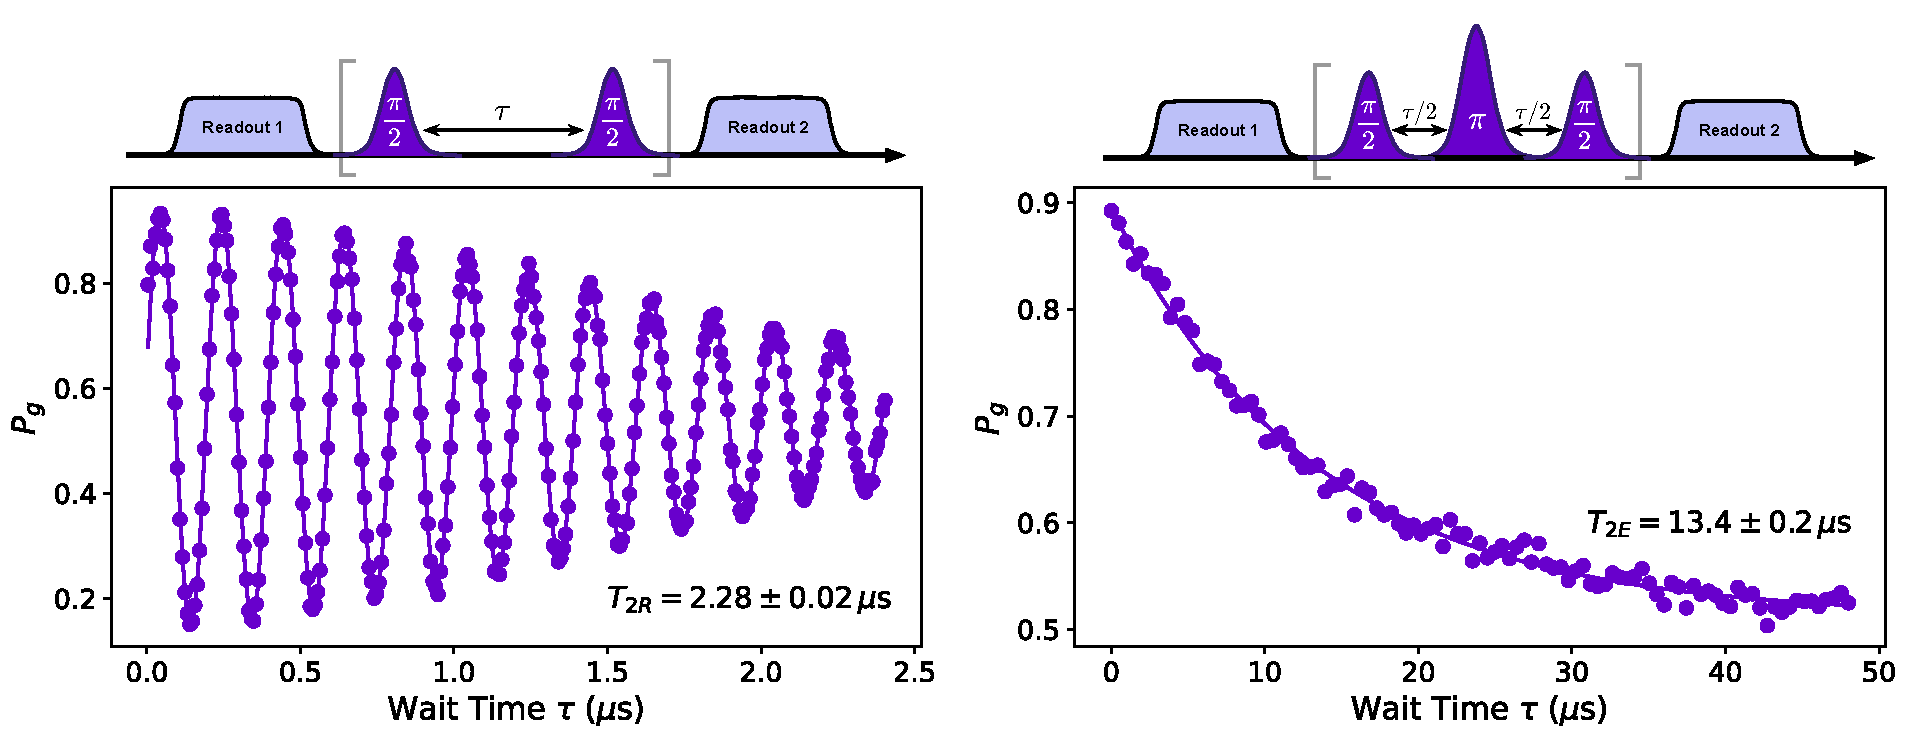
\includegraphics[width=\linewidth]{Figures/4/T2_ramsey_echo.pdf}
    \caption[Qubit \texorpdfstring{$T_2$}{T2} Ramsey and Echo measurements.]{$T_2$ measurements for our fluxonium at half-flux. \textbf{(a)} The Ramsey experiment reveals $T_{2R} = 2.28 \pm 0.02$ $\mu$s. Oscillation fringes were introduced by detuning the qubit pulses from the qubit frequency. \textbf{(b)} The Echo measurement reveals $T_{2E} = 13.4 \pm 0.2$ $\mu$s. }
    \label{fig:4_T2_ramsey_echo}
\end{figure}

% \todo{Perhaps mention flux noise amplitude if there is space for it.}

\clearpage
\section{Storage Resonator Measurements \label{sec:4_StorageChi}}

\subsection{Storage Spectroscopy}

We are now ready to discuss measurements of the storage resonator. At this stage, we had already identified the storage in two-tone spectroscopy, and now wanted to corroborate this using a storage spectroscopy experiment. This measurement uses the qubit as a meter to probe the storage resonator frequency; as shown below in Fig. \ref{fig:4_storage_spectroscopy}, it involves driving the storage resonator and then performing a frequency-selective $\pi$-pulse on the qubit. This $\pi$-pulse is chosen to have length $\tau \gg 1/\chi_{qs}$ and a frequency that corresponds to the qubit frequency when the storage has zero photons. When the initial storage drive is resonant with the cavity, it will displace the storage away from the vacuum $\ket{0}$; as a result, the $\pi$ pulse fails. Only when the storage drive is off-resonant will the cavity remain in its $\ket{n=0}$ state, and thus cause the $\pi$-pulse to be implemented correctly. Finally, given our need for post-selection here, we can initialize the fluxonium in either $\ket{g}$ or $\ket{e}$ to see two different resonance dips. In practice, we used a constant $\tau = 2.4$ $\mu$s for the selective pulse.
\begin{figure}[h]
    \centering
    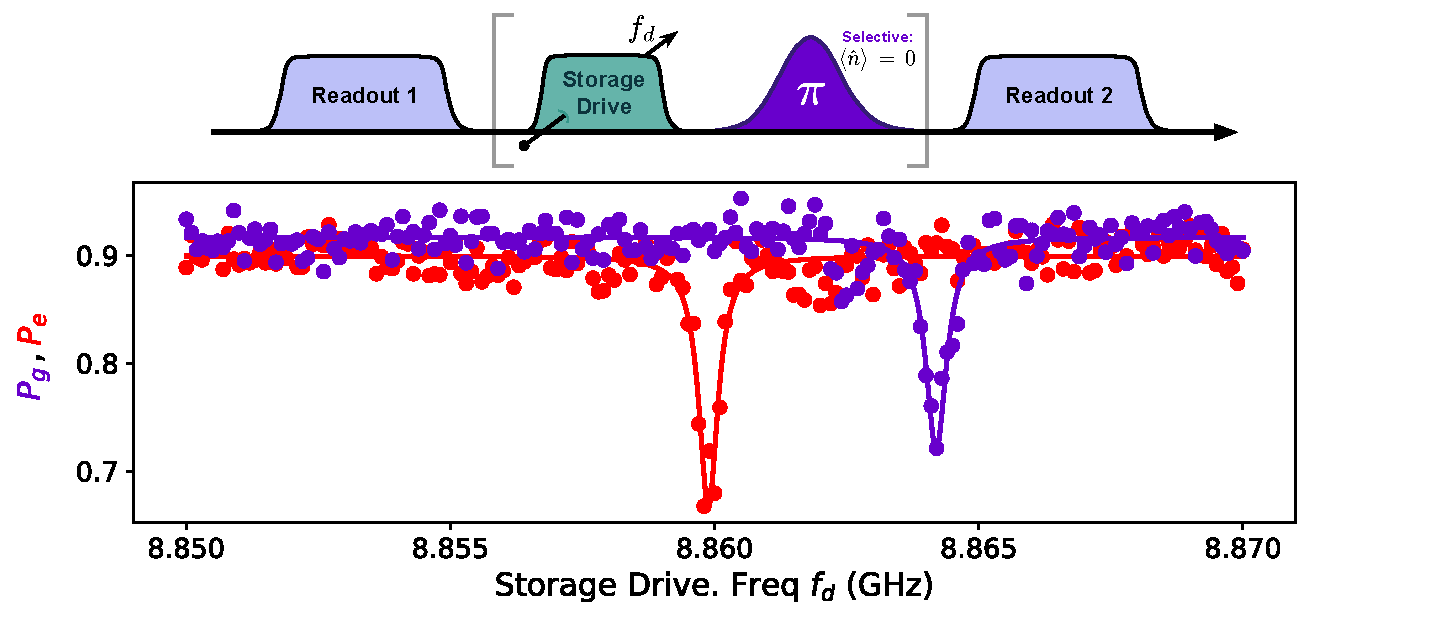
\includegraphics[width=0.85\linewidth]{Figures/4/storage_spectroscopy.pdf}
    \caption[Storage spectroscopy measurement.]{Storage spectroscopy measurement via the qubit. This experiment enables us to determine the storage frequency when the qubit is in $\ket{g}$ or $\ket{e}$ respectively.}
    \label{fig:4_storage_spectroscopy}
\end{figure}

\subsection{Engineering a Tunable Dispersive Shift}

The storage spectroscopy measurement above presents a method to extract the dispersive shift $\chi_{qs}$ between the fluxonium and storage. We simply sweep the external flux $\Phi_{\rm ext}$ and tune up a frequency-selective $\pi$-pulse at each bias point. Since the storage flux dispersion is minimal, we can perform a storage spectroscopy at each flux, and calculate $\chi_{qs}$ as the difference in the resonance frequency when the qubit is in $\ket{g}$ vs. $\ket{e}$, as is consistent with a Hamiltonian coupling term $\chi_{qs} \hat{a}^\dagger\hat{a}\sigmaz/2$. The result of this measurement is shown in Fig. \ref{fig:4_tunable_chi}, and we see that the dispersive shift indeed tunes with flux and crosses through zero, as is expected with bosonic mode threading. This is one of the central results of this thesis.

\begin{figure}[h]
    \centering
    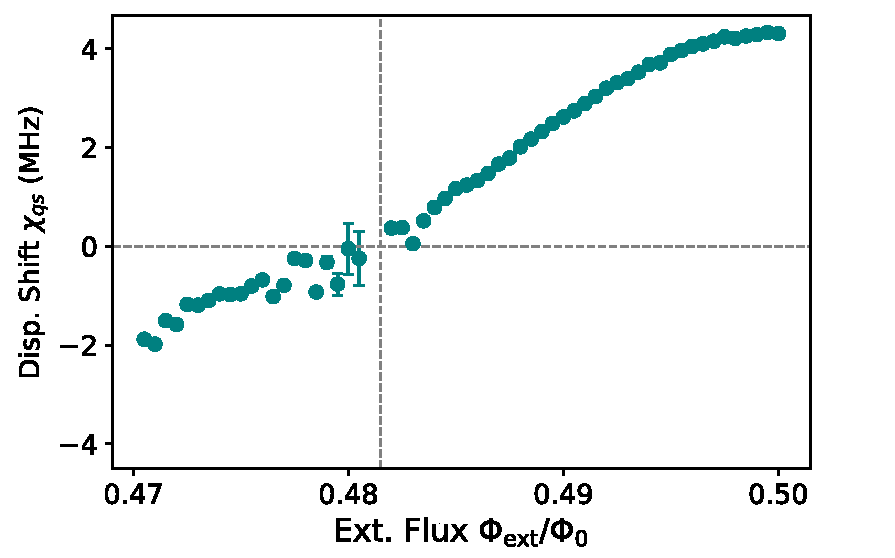
\includegraphics[width=0.6\linewidth]{Figures/4/tunable_chi.pdf}
    \caption[Demonstration of a flux-tunable storage dispersive shift.]{Measurement of the tunable storage dispersive shift $\chi_{qs}(\Phi_{\rm ext})$ vs. the external flux $\Phi_{\rm ext}$. We mark the approximate zero crossing point, which occurs at $\Phi_{\rm ext} \approx 0.481\Phi_0$.}
    \label{fig:4_tunable_chi}
\end{figure}

Given that we used a selective $\pi$-pulse of the same length $\tau = 2.4$ $\mu$s at each flux point, we do not expect this measurement technique to work well near the zero crossing point where $\chi_{qs} \to 0$, since there the condition $\tau \gg 1/\chi_{qs}$ ceases to hold. We thus see slightly larger error bars at the crossing and cannot measure the exact point at which $\chi_{qs}=0$ (the fit fails there). Nonetheless, we have the desired upshot of being able to toggle the qubit-storage interaction with flux. 

\clearpage

\section{Storage Coherence: Problems and Pitfalls \label{sec:4_StorageCoherenceProblems}}

Our next experimental step was to characterize the coherence of the storage resonator. As we later discovered, however, the storage lifetime was severely limited in our device. This led to a series of A/B tests and many months of debugging before we realized that the problem was in some sense inherent to our design. In this section, we will present some of the major clues that led us to this conclusion. 

\subsection{Initial Time-Domain Measurement}

The first method we took to measure the storage lifetime was based on a number-splitting spectroscopy experiment \cite{schuster2007resolving}. This measurement sequence uses a selective qubit $\pi$-pulse, and in particular consists of playing a storage drive at one of the storage peaks (e.g. $\omega_s^{\ket{g}}$) and then performing qubit spectroscopy with the selective pulse. If we post-select to have started with the qubit in $\ket{g}$, then this will enable us to see multiple resonance peaks in the qubit spectrum corresponding to the photon number distribution in the cavity after it is excited via the storage pulse. We can see an example of this on the left plot in Fig. \ref{fig:4_storage_T1_numsplit} below, which shows the photon number distribution (teal) after driving the storage with a 10 $\mu$s pulse, followed by a 2.4 $\mu$s selective qubit $\pi$-pulse. The distribution is specified via the depth of the various resonance dips, and is expected to follow a Poisson distribution as the storage is driven to a coherent state. We contrast this with the case when the storage pulse is not played (grey), resulting in just a single qubit spectroscopy dip corresponding to the storage having $\ket{n=0}$ photons. 

In order to measure the storage $T_1$ this way, we can introduce a variable delay between the storage drive pulse and the qubit $\pi$-pulse. During this time, the storage will experience photon loss $\kappa_{1s}\mathcal{D}[\hat{a}]$ and thus the number distribution will decay back down towards the vacuum. We can measure this decay by parking at, say, the $\ket{n=0}$ dip and recording the change in contrast vs. time. For single-photon loss rate $\kappa_{1s}$, we expect an initial coherent state $\alpha_0$ to decay as $\alpha(t) = \alpha_0 e^{-\kappa_{1s}t/2}$, i.e., so that $\bar{n}(t) = |\alpha(t)|^2 =  \bar{n}_0 e^{-\kappa_{1s}t}$ with $\bar{n}_0 = |\alpha_0|^2$. We can fit the decay of the $\ket{n=0}$ qubit spectroscopy dip by weighting $\bar{n}(t)$ via the Poisson distribution evaluated at $n = 0$. This gives us a fit function $P_{g, 0}(t) = 1-a\cdot\exp[-\bar{n}_0 e^{-\kappa_{1s}t}]$ for the decay, where $a$ is a scale parameter to account for the partial contrast. From this, we can extract the lifetime $T_{1s} = 1/\kappa_{1s}$. We show the result of such a measurement in the right panel of Fig. \ref{fig:4_storage_T1_numsplit}.
\begin{figure}[h]
    \centering
    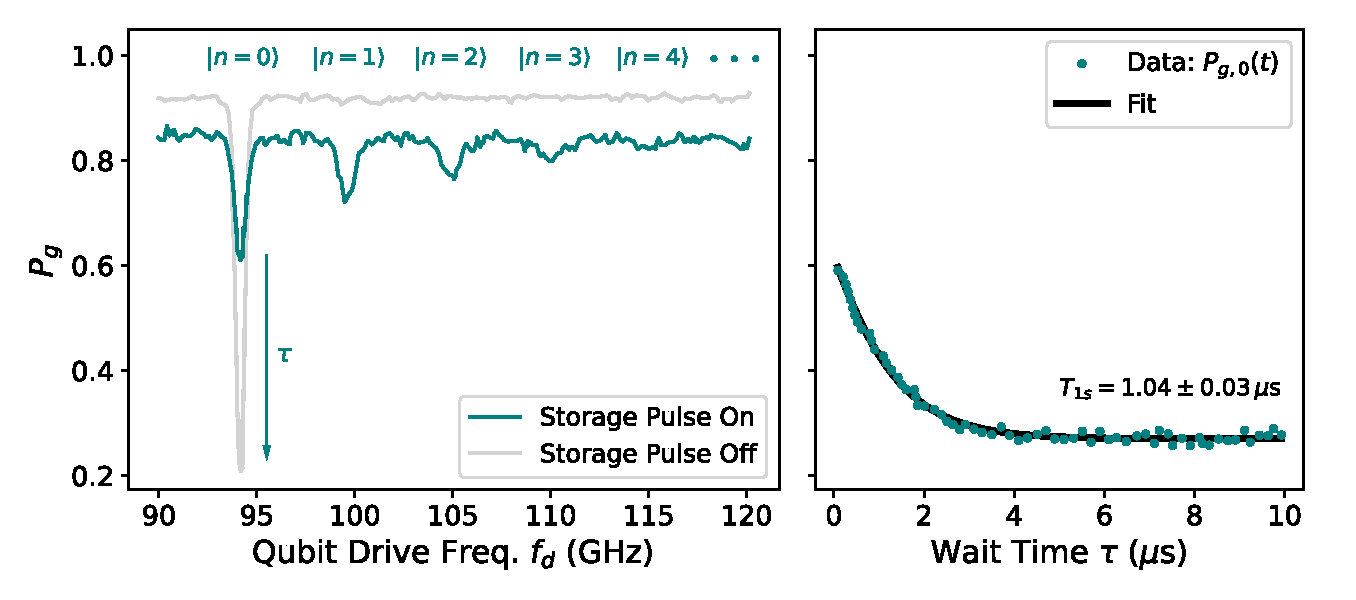
\includegraphics[width=\linewidth]{Figures/4/storage_T1_numsplit.pdf}
    \caption[Qubit spectroscopy in the photon-number resolved regime and time-domain measurement of the storage resonator \texorpdfstring{$T_1$}{T1} lifetime.]{Left: Number-splitting spectroscopy data for the qubit at half-flux, showing multiple photon-resolved dips (teal) after driving the storage for 10 $\mu$s. If we add a variable delay after the storage pulse, we observe the number distribution decaying back towards the case when the storage has $\ket{n=0}$ photons (grey). Plotting the depth of the $\ket{n=0}$ dip vs. time allows us to measure the single-photon decay and extract the storage lifetime.}
    \label{fig:4_storage_T1_numsplit}
\end{figure}

\subsection{Testing and Progress}
We were very surprised to measure a storage lifetime of $T_{1s} \approx 1$ $\mu$s, given the bare lifetime of the Mark II storage cavity of $T_{1s}^{\rm bare} \approx 765$ $\mu$s that we had seen previously without qubit chips. We therefore set out to debug this part of our system over several subsequent cooldowns. In time, we were able to verify that our bare 3D cavity resonators indeed had high coherence; we tested both the Mark II and Mark III cavities in various configurations as shown in Fig. \ref{fig:4_3D_Cavity_Debugging}. These tests also helped us rule out excess coupling loss due to the storage drive pin. One observation we made is that even inserting blank Si chips (i.e., with no qubit, flux line, or metallization) into the cavities seemed to degrade their lifetime from above 1 ms to approximately 100 $\mu$s. We attributed this to lossy backside of the qubit chip, since the Si wafer used to fabricate the fluxonium devices was only single-side polished\footnote{This was an aberration in the fabrication process used for our devices, since the 8" Si process was still being developed at that time. One should otherwise always use a double-side polished wafer since the backside of the chip can also introduce unwanted dielectric losses!}. Nonetheless, this effect alone was not enough to account for the drop in cavity coherence from over 760 $\mu$s to $\sim\!1$ $\mu$s. 

\begin{figure}[t]
    \centering
    \includegraphics[width=\linewidth]{Figures/4/3D_Cavity_Debugging.pdf}
    \caption[Attempts to debug low storage lifetime in different configurations.]{Maximum single-photon $T_{1s}$ measured across all three resonators of the Mark III cavity. We calculate $T_{1s}$ using low-power frequency-domain measurements with a Vector Network Analyzer. Each configuration was tested during a different cooldown of the fridge.}
    \label{fig:4_3D_Cavity_Debugging}
\end{figure}

Our main suspicion was that the storage loss was coming primarily from the qubit flux line; we thus first attempted to remedy it by adding external DC/RF filtering to our lines. Unfortunately, this is did not seem to solve the problem. We later also attempted capping the flux line with a 50 $\Omega$ terminator and then went as far as fully de-wirebonding it; neither of these changes helped appreciably and the storage lifetime remained around 1 $\mu$s or less. Our conclusions from these tests were also muddied by uncontrolled factors between the various cooldowns (e.g., statistical variations in lifetime, degradation of the cavities with time, or changes to the exact amount of indium used in the seals). 

\subsection{Direct Measurement of Loss from the Flux Line}

We were ultimately able to confirm our suspicions about the flux line loss by performing a direct reflection ($S_{11}$) measurement of the 3D cavities \textit{through} the flux lines. We connected a VNA to the flux line and were able to measure the storage cavity resonance, which alone was enough to tell us that the flux line was too strongly coupled (cf. Fig. \ref{fig:4_storage_loss_thru_flux_line}); we ideally should not be able to see anything. Here, however, the low-power resonator spectroscopy measurement shows two dips associated with the qubit being in $\ket{g}$ or $\ket{e}$ respectively (since we had the flux line connected and biased near half-flux). To reflect this, we fitted the data to a double Lorentzian $S_{11}$ model consisting of two weighted peaks with identical linewidths but different frequencies. From here, we were able to extract $\kappa_c/2\pi = 320.9$ kHz and $\kappa_i/2\pi = 2.03$ MHz. 

\begin{figure}[h]
    \centering
    \includegraphics[width=0.7\linewidth]{Figures/4/storage_loss_thru_flux_line.pdf}
    \caption[Direct measurement of the storage resonator through the qubit flux line.]{Direct measurement of the storage resonance through the qubit flux line. At half-flux, we see two peaks associated with the states $\ket{g}$ and $\ket{e}$. We fit data to a double Lorentzian $S_{11}$ model with two weighted peaks of identical linewidth to extract $\kappa_c$ and $\kappa_i$.}
    \label{fig:4_storage_loss_thru_flux_line}
\end{figure}

In the configuration of measuring $S_{11}$ through the flux line, the constant $\kappa_c$ tells us how much of the total storage loss comes from its coupling to the flux line. We get $T_{1c} = 1/\kappa_c \simeq 0.496$ $\mu$s, thus confirming that the flux line is limiting. However, in this measurement, we found that the internal loss $\kappa_i$ is even larger than $\kappa_c$, suggesting there is \textit{another} loss channel at play beyond just the flux line. 

\subsection{Storage Loss HFSS Simulations and Summary}

We were finally able to resolve the storage loss question by revisiting our E\&M eigenmode simulations of the 3D cavity package using Ansys-HFSS\footnote{I'd like to thank R\'eouven Assouly for his insight to re-run the simulations, for various tips for using HFSS, and his help and willingness to brainstorm creative solutions during this turbulent time in the project.}. We found that the storage losses were significant even in simulation and thus inherent to our design. This is ultimately the reason why many of the steps we took during our A/B testing did not improve the cavity lifetimes. We show an example simulation in Fig. \ref{fig:4_HFSS_Simulation}, here characterizing the effect of 50 $\Omega$ loss from the flux line [panel (a)]. We consistently found that when the fluxonium chip is inserted, the electric field of the storage mode does \textit{not} stay confined to the post cavity, but instead `leaks out' and does so in two distinct ways: (i) through the qubit flux line, as shown in panel (d), and (ii) by participating in the ground plane mode between the chip and the tunnel walls, as shown in panel (e). We found in simulation that the former effect (i) seemed to depend significantly on the shape of the flux line tip. In particular, using an exact model of the flux line [Fig. \ref{fig:4_HFSS_Simulation}(b)] resulted in a storage lifetime of $T_{1s} \simeq 0.5$ $\mu$s in simulation, whereas using an approximate model [Fig. \ref{fig:4_HFSS_Simulation}(c)] gave a lifetime of $T_{1s} \simeq 1.9$ ms --- roughly four orders of magnitude higher! This discrepancy is likely the reason why we did not catch this error during the initial design/simulation of the 3D cavity system; in turn, this resulted in significant storage loss down the flux line that we saw in experiment and showed in Fig. \ref{fig:4_storage_loss_thru_flux_line}.

\begin{figure}[t]
    \centering
    \includegraphics[width=0.8\linewidth]{Figures/4/HFSS_Simulation.pdf}
    \caption[HFSS electromagnetic simulations of the 3D cavity-fluxonium architecture showing storage losses inherent to the design.]{\textbf{(a)} HFSS model of our 3D cavity-fluxonium device with a 50 $\Omega$ loss channel. \textbf{(b, c)} Exact and approximate models for the tip of the flux line. \textbf{(d)} Eigenmode simulation result showing storage cavity electric field; the field is mostly concentrated around the post cavity, but also leaks down the flux line. \textbf{(e)} Different angle showing the cavity field also participating in the ``ground plane'' mode, and thus leading down the chip tunnel.}
    \label{fig:4_HFSS_Simulation}
\end{figure}

As the experimental data also suggested, however, the latter source of loss due to storage participation in the ground plane mode was also significant, and thus something we tried to reproduce in simulation. This effect (ii) is more subtle, and arises when a voltage develops between the ground plane metallization of the qubit chip and the tunnel wall of the 3D cavity, giving rise to a $(\lambda/4)$-like mode of the entire ground plane. The storage participates in this spurious mode and thus its field can be thought to `leak' down the tunnel. As a result, the storage will experience a full litany of loss mechanisms that 3D cavities are otherwise supposed to be resilient to by design (e.g., seam loss at the mouth of the tunnel and mode participation in lossy glue and/or PCB dielectrics) \cite{reagor2013reaching,brecht2015demonstration,reagor2016quantum}. We corroborated this in simulation by later including seam loss explicitly. From these simulations, we realized that the ``ground plane'' loss channel (ii) will always arise if there is significant metallization inside the chip tunnel. While this could in principle be alleviated by somehow grounding the chip to the 3D cavity tunnel walls (e.g., using indium), doing so would necessarily also introduce seam losses, and thus it is not immediately clear how to proceed. Meanwhile, the ``flux line'' loss (i) could be solved in several ways, such as by using some form of on-chip microwave filtering \cite{pozar2012microwave} (more discussion of this in Ch. \ref{ch:5_2DGKP}).  

In summary, we learned from our experiments that it is a difficult technical challenge to integrate a fast-flux line in 3D while maintaining the coherence of an otherwise high-Q cavity. Although this presents a major hurdle for using fluxonium in a 3D-cavity architecture for the purpose of bosonic QEC, there are potential paths forward. We will discuss a few such approaches in the upcoming chapter. 

\clearpage
\printbibliography[heading=subbibliography, title = References]
\printbibliography[heading=subbibliography, title = References]
\clearpage
% % ------------------------------------------------

% %%%%% Chapter 5: Next Steps and 2D GKP %%%%%%
\chapter{Next Steps and Moving to 2D\label{ch:5_2DGKP}}


In the previous chapter, we presented the results of our experiments with a fluxonium in a 3D cavity. We demonstrated a tunable dispersive shift between the qubit and the storage resonator via bosonic mode threading and characterized the various components of our system. In doing so, we discovered that the lifetime of the storage mode was \textit{significantly} lower than expected (as compared to its bare value) whenever the qubit chip was inserted into the resonator package. After many rounds of experimentation and testing, we were ultimately able to attribute this effect to two main sources: (i) the storage mode's coupling to the lossy qubit flux line; and (ii), its participation in spurious modes of the 3D superconducting package. While the former issue could in principle be solved via clever microwave engineering and filtering, the latter unfortunately is intrinsic to our 3D design and not easily remedied. As we came to learn, it is generally difficult to integrate fast-flux into a 3D cavity while also maintaining the cavity coherence. 

There are certain approaches that have been proposed and implemented in the literature that work towards integrating fast-flux in 3D. One such example is the magnetic hose from Refs. \cite{gargiulo2021fast,valadares2023demand}. Here, the authors route flux from an external coil to a tunable transmon qubit in a 3D superconducting package using a ``hose'' composed of concentric aluminium and mu-metal layers. In the experiment of Ref. \cite{valadares2023demand} specifically, this is done for the purpose of bosonic cQED, and the authors demonstrate that the lifetime of their 3D storage resonator is not limited by their flux delivery mechanism. Unfortunately, however, the design and implementation of a magnetic hose is quite painstaking, and would require a full redesign of both the cavities and the fluxonium chips that were presented in Ch. \ref{ch:4_3DGKP}. Other designs have also been proposed recently, e.g. Ref. \cite{hutin2024monitoring} or Ref. \cite{maiti2024ancilla}, which both rely on some form of on-chip distributed-element microwave filtering to prevent losses from the flux line at the frequency of the storage. Despite requiring more advanced microwave engineering in design, these approach seem promising for integrating fast-flux in 3D while maintaining the storage resonator lifetime. 

In our case, however, after discovering the root cause of our storage coherence issues and identifying various avenues to proceed from there, we decided to forgo the 3D architecture entirely. This was in part due to the time and difficulty of implementing fast-flux delivery in 3D (which, as highlighted above, is a difficult project in of itself); but it was also a choice we made consciously, motivated by the idea of moving our experiments to 2D. Over the course of our 3D-GKP project, we ended up developing an entirely separate but novel way to do GKP error correction in 2D, using a microwave-activated coupler to generate faster conditional displacements. This 2D project, first proposed using a transmon control qubit and later a fluxonium, represents an improvement over the ``direct dispersive'' approach we took in our 3D-GKP project in most ways. As such, we decided that moving to 2D is a more promising long term path towards building extensible GKP error correction systems. 

In this chapter, we present three of our proposals for implementing GKP error correction in 2D. Within our bosonic subgroup in EQuS, we refer to these as the ``RAT'' (see Ch. \ref{sec:5_RAT}), the ``RAF'' (see Ch. \ref{sec:5_RAF}), and the ``2D dispersive'' (see Ch. \ref{sec:5_2D_Disp}) approaches, respectively\footnote{The meaning behind these names will become apparent shortly!}. We will go through the basic theory for all three approaches and discuss high-level results. In particular, we have already completed designs for the RAF and 2D dispersive projects, which are currently being fabricated as of this writing. 

Here, my aim is give a broad overview to our upcoming 2D experiments; however, more details and a discussion of the careful design and simulation considerations taken can be found in the SM thesis of Shantanu Jha. 
\clearpage


\section{The Asymmetrically-Threaded-SQUID Coupler \label{sec:5_RAT}}

The core insight that motivated our investigation into GKP error correction in 2D was that we can use an Asymmetrically-Threaded SQUID (ATS) as a coupler element to realize the desired ``three-wave mixing'' conditional displacement term that underpins all GKP QEC schemes. The ATS is a superconducting dipole element consisting of a symmetric SQUID shunted by an inductor, as shown in Fig. \ref{fig:5_ats_spectrum}(a); the two resulting flux loops in the circuit are then typically biased \textit{asymmetrically} \cite{lescanne2020exponential, berdou2023one}. In practice, the inductor is realized using an array of Josephson junctions and so the circuit itself is similar to that of a gradiometric SNAIL \cite{miano2022frequency}; it was also recently referred to as the Linear Inductive Coupler when biased symmetrically \cite{maiti2024ancilla}. Despite these various names, we will refer to the actual dipole element as an ATS throughout our work, irrespective of its bias point. 

\begin{figure}[h]
    \centering
    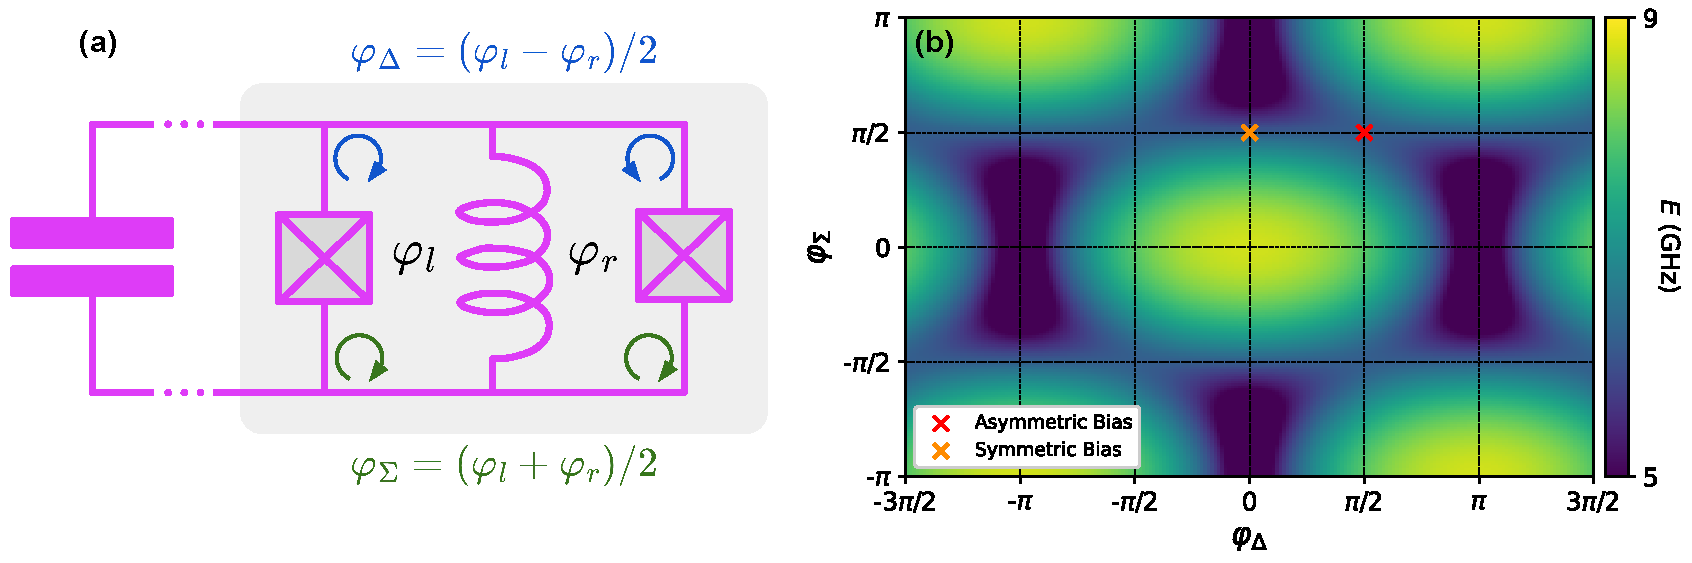
\includegraphics[width=\linewidth]{Figures/5/ats_spectrum.pdf}
    \caption{\textbf{(a)} Circuit diagram for the ATS dipole element (shaded in gray) which consists of a symmetric SQUID shunted by an inductor. The left/right loops are threaded by fluxes $\varphi_l$/$\varphi_r$ respectively, giving rise to common and differential fluxes $\varphi_\Sigma$ and $\varphi_\Delta$. When the ATS is connected to a capacitor, it forms a mode. \textbf{(b)} Fundamental frequency of the ATS mode vs. flux $(\varphi_\Sigma, \varphi_\Delta)$ using parameters $E_L/h = 60$ GHz, $E_J/h = 30$ GHz, and $E_C/h = 80$ MHz.}
    \label{fig:5_ats_spectrum}
\end{figure}

\noindent To begin our exploration of the ATS, let's consider its potential energy, which is given by:
\begin{equation}
    \hat{U}_b = \frac{1}{2}E_L \bigg(\hat{\varphi} + \frac{C_r\varphi_r - C_l\varphi_l}{C_\Sigma}\bigg)^2 - E_{J,l}\cos\!\bigg(\hat{\varphi} + \frac{C_r}{C_\Sigma}[\varphi_l + \varphi_r]\bigg) - E_{J,r}\cos\!\bigg(\hat{\varphi} - \frac{C_l}{C_\Sigma}[\varphi_l + \varphi_r]\bigg)
\end{equation}
Here, we have used the method of Ref. \cite{you2019circuit} to write the potential in terms of its irrotational variable $\hat{\varphi}$, which is the correct approach for time-varying external fluxes; the expression is thus somewhat different from the original description of the ATS in Ref. \cite{lescanne2020exponential}. We have left and right junctions with energies $E_{J, l/r}$, inherent capacitances $C_{l/r}$, and external fluxes $\varphi_{l/r}$ respectively. At this point, we can define the effective $E_J = (E_{J,l} + E_{J,r})/2$ and asymmetry $\Delta E_J = (E_{J,l} - E_{J,r})/2$, and transform to sum and difference coordinates $\varphi_{\Sigma/\Delta} = (\varphi_l \pm \varphi_r)/2$.  Ideally, we would like the junctions to be perfectly symmetric; in practice the asymmetry can be minimized to about $1\%$ of $E_J$. While this is important to keep track of, we will here set $\Delta E_J \to 0$ in the rest of the theory that follows. Thus, $E_{J,l} = E_{J,r} = E_J$ and $C_l = C_r = C$, with $C_\Sigma = C_l + C_r$. We can therefore simplify the complicated expression above and write the potential as:
\begin{equation}
\hat{U}_b(\hat{\varphi}) = \frac{1}{2}E_L(\hat{\varphi} - \varphi_\Delta)^2 - 2E_J \cos(\varphi_\Sigma)\cos(\hat{\varphi})
\end{equation}
In what follows, we will typically keep the differential flux $\varphi_\Delta$ constant and only modulate the common flux $\varphi_\Sigma = \varphi_\Sigma(t)$. Therefore, we can perform a gauge transformation to move the now DC flux $\varphi_\Delta$ to the cosine via $\hat{\varphi} \mapsto \hat{\varphi} + \varphi_\Delta$. This finally get us back to the familiar expression
\begin{equation}
\hat{U}_b(\hat{\varphi}) = \frac{1}{2}E_L\hat{\varphi}^2 - 2E_J \cos(\varphi_\Sigma)\cos(\hat{\varphi} + \varphi_\Delta)
\end{equation}
that can be found in Refs. \cite{lescanne2020exponential, berdou2023one}. We will use this throughout the rest of this chapter.

As shown in Fig. \ref{fig:5_ats_spectrum}(b), when the ATS is connected to a capacitance, the resulting mode has a fundamental frequency that is doubly periodic in $\varphi_\Sigma$ and $\varphi_\Delta$, forming an `egg-carton' potential as it is sometimes referred to. There are two typical operating points for the ATS:

\begin{itemize}
    \item \textbf{Asymmetric bias point:} $(\varphi_\Sigma, \varphi_\Delta) = (\pi/2, \pi/2)$, corresponding to $\varphi_l = \pi$ and $\varphi_r = 0$. This is the standard operating point for the ATS. By modulating the sum flux around this bias, i.e. $\varphi_\Sigma(t) = \pi/2 + \epsilon(t)$, we get the following time-dependent potential for the ATS dipole:
    \begin{equation}
        \hat{U}_b(\hat{\varphi}) = \frac{1}{2}E_L \hat{\varphi}^2 - 2E_J \sin[\epsilon(t)]\sin(\hat{\varphi})
    \end{equation}
\item \textbf{Symmetric bias point:} $(\varphi_\Sigma, \varphi_\Delta) = (\pi/2, 0)$, corresponding to $\varphi_l = \varphi_r = \pi/2$. Biasing here gives us:
\begin{equation}
        \hat{U}_b(\hat{\varphi}) = \frac{1}{2}E_L \hat{\varphi}^2 - 2E_J \sin[\epsilon(t)]\cos(\hat{\varphi})
    \end{equation}
\end{itemize}
%%%%%%%%%%%%%%%%%%%%%%%%
\subsection{The Resonator-ATS-Transmon (RAT)}

Our first approach to faster GKP error correction was developed using the ATS as a coupler element between a storage resonator and a transmon control qubit. We name this the RAT. The basic idea relies on black-box quantization (cf. Ch. \ref{ch:3_cQED}) between the three modes $\hat{a}_0$, $\hat{b}_0$, and $\hat{q}_0$ for the resonator, ATS, and transmon respectively. The bare transmon Hamiltonian is:
\begin{equation}
\hat{H}_{q, 0} = 4E_{C,q}\hat{n}_q^2 - E_{J,q}\cos(\hat{\theta}) = \omega_{q,0}\,\hat{q}_0^\dagger \hat{q}_0 - \Big[E_{J,q}\cos(\hat{\theta}) + \frac{1}{2}E_{J,q} \hat{\theta}^2\Big] 
\end{equation}
where we write the mode $\hat{q}_0$ in terms of the transmon charge $\hat{n}_q$ and phase-drop $\hat{\theta}$. For the ATS, it is:
\begin{equation}
\hat{H}_{b,0} = 4E_C \hat{n}^2 + \hat{U}_b(\hat{\varphi}) = \omega_{b,0}\hat{b}_0^\dagger \hat{b}_0 - 2E_J \cos(\varphi_\Sigma)\cos(\hat{\varphi} + \varphi_\Delta)
\end{equation}
in terms of the ATS charge operator $\hat{n}$ and phase-drop $\hat{\varphi}$. Finally, for the storage we have $\hat{H}_{a, 0} = \omega_{a,0}\hat{a}_0^\dagger \hat{a}_0$. If we take the modes to be linearly coupled (e.g. via capacitive coupling) in series, i.e. resonator $\leftrightarrow$ ATS $\leftrightarrow$ transmon, then the total Hamiltonian has a \textit{linear} part:
\begin{equation}
\hat{H}_{\rm lin, 0} = \omega_{a,0}\hat{a}_0^\dagger \hat{a}_0 + \omega_{b,0}\hat{b}_0^\dagger \hat{b}_0 + \omega_{q,0}\hat{q}_0^\dagger \hat{q}_0 - g_{ab}(\hat{a}_0 - \hat{a}_0^\dagger)(\hat{b}_0 - \hat{b}_0^\dagger) - g_{qb}(\hat{b}_0 - \hat{b}_0^\dagger)(\hat{q}_0 - \hat{q}_0^\dagger)
\end{equation}
Following black-box quantization, we can diagonalize $\hat{H}_{\rm lin, 0}$ as a system of normal modes $\hat{a}$ (storage-like), $\hat{b}$ (buffer-like), and $\hat{q}$ (qubit-like). In this basis $\hat{H}_{\rm lin} = \omega_a \hat{a}^\dagger\hat{a} + \omega_b \hat{b}^\dagger\hat{b} + \omega_q \hat{q}^\dagger\hat{q}$, where $\omega_a$, $\omega_b$, and $\omega_q$ are the normal mode frequencies. We can also rewrite the bare modes in this normal mode basis via a linear transformation:
\begin{align}
\hat{\theta} &= \theta_{q, 0}(\hat{q}_0 + \hat{q}_0^\dagger) = \theta_q(\hat{q} + \hat{q}^\dagger) + \theta_b(\hat{b} + \hat{b}^\dagger) + \theta_a(\hat{a} + \hat{a}^\dagger) \\
\hat{\varphi} &= \phi_{b, 0}(\hat{b}_0 + \hat{b}_0^\dagger) = \phi_q(\hat{q} + \hat{q}^\dagger) + \phi_b(\hat{b} + \hat{b}^\dagger) + \phi_a(\hat{a} + \hat{a}^\dagger)
\label{eq:linear_basis_RAT_RAF}
\end{align}
Here, $\theta_i$ denotes the participation of mode $i$ in the phase across the Josephson junction in the transmon, while $\phi_i$ is the participation in the phase across the ATS. In total, we have
\begin{equation}
\hat{H} = \sum_{c = \{a, b, q\}}\omega_c \hat{c}^\dagger\hat{c} - \Big[E_{J,q}\cos(\hat{\theta}) + \frac{1}{2}E_{J,q} \hat{\theta}^2\Big] - 2E_J \cos(\varphi_\Sigma)\cos(\hat{\varphi} + \varphi_\Delta)
\end{equation}
as the Hamiltonian for the full resonator-ATS-transmon system written in the ``black-box quantization'' basis (i.e. of the normal modes of the linearized circuit). 

With the Hamiltonian written down, let's now see how to get conditional displacements out of it. We park the ATS at its standard asymmetric bias point $(\varphi_\Sigma, \varphi_\Delta) = (\pi/2, \pi/2)$ and modulate $\varphi_\Sigma(t) = \pi/2 + \epsilon(t)$ about this. The ATS potential takes on the form $\sin[\epsilon(t)]\sin(\hat{\varphi})$, and so we can Taylor expand $\sin[\epsilon(t)] \approx \epsilon(t)$ and $\sin(\hat{\varphi}) \approx \hat{\varphi} - \hat{\varphi}^3/6$ in anticipation of making a rotating-wave approximation. We can also truncate the transmon potential to a Duffing oscillator, considering only the leading fourth-order nonlinearity. These approximations give us
\begin{equation}
\hat{H} = \sum_{c = \{a, b, q\}}\omega_c \hat{c}^\dagger\hat{c} - \frac{E_{J,q}}{24}\hat{\theta}^4 - 2E_J \epsilon(t)\hat{\varphi} + \frac{1}{3}E_J\epsilon(t)\hat{\varphi}^3
\end{equation}
We go into a rotating frame for each of the modes $\hat{c} \mapsto \hat{c} e^{-i\tilde{\omega}_c t}$ where we set the frequency $\widetilde{\omega}_c = \omega_c - \theta_{c}^{2} \big[\theta_{a}^{2} + \theta_{b}^{2} + \theta_{q}^{2}\big]/2$ to cancel out the frequency normalizations that arise from the transmon nonlinearity. In this frame, we get
\begin{align}
\begin{split}
\hat{H} &= \hat{H}_{cc} - \frac{E_{J,q}}{24}\Big[\theta_q(\hat{q}e^{-i\tilde{\omega}_q t} + \hat{q}^\dagger e^{i\tilde{\omega}_q t}) + \theta_b(\hat{b}e^{-i\tilde{\omega}_b t} + \hat{b}^\dagger e^{i\tilde{\omega}_b t}) + \theta_a(\hat{a}e^{-i\tilde{\omega}_a t} + \hat{a}^\dagger e^{i\tilde{\omega}_a t})\Big]^4 \\&\quad- 2E_J\epsilon(t)\Big[\phi_q(\hat{q}e^{-i\tilde{\omega}_q t} + \hat{q}^\dagger e^{i\tilde{\omega}_q t}) + \phi_b(\hat{b}e^{-i\tilde{\omega}_b t} + \hat{b}^\dagger e^{i\tilde{\omega}_b t}) + \phi_a(\hat{a}e^{-i\tilde{\omega}_a t} + \hat{a}^\dagger e^{i\tilde{\omega}_a t})\Big]\\ &\quad + \frac{1}{3}E_J\epsilon(t)\Big[\phi_q(\hat{q}e^{-i\tilde{\omega}_q t} + \hat{q}^\dagger e^{i\tilde{\omega}_q t}) + \phi_b(\hat{b}e^{-i\tilde{\omega}_b t} + \hat{b}^\dagger e^{i\tilde{\omega}_b t}) + \phi_a(\hat{a}e^{-i\tilde{\omega}_a t} + \hat{a}^\dagger e^{i\tilde{\omega}_a t})\Big]^3
\end{split}
\end{align}
where $\hat{H}_{cc} = \sum (\omega_c - \tilde{\omega}_c)\hat{c}^\dagger\hat{c}$ will cancel out when the terms are expanded. At this point our task involves sorting through the various pumped nonlinear terms and keeping only the ones that survive the RWA. We set $\epsilon(t) = \epsilon_p \sin(\omega_p t)$ with $\omega_p = \tilde{\omega}_a$, picking out terms that rotate at the (renormalized) storage frequency. Luckily we can do the oscillator expansion, normal ordering, and RWA all numerically using SymPy. The final effective Hamiltonian
\begin{align}
\begin{split}
\hat{H}_{\rm eff} &= \frac{K_a}{2}{{a}^\dagger}^{2} {a}^{2} + \frac{K_b}{2}{{b}^\dagger}^{2} {b}^{2} + \frac{K_q}{2}{{q}^\dagger}^{2} {q}^{2} + \frac{\chi_{ab}}{2}\hat{a}^\dagger\hat{a}\hat{b}^\dagger\hat{b} + \frac{\chi_{aq}}{2} \hat{a}^\dagger\hat{a}\hat{q}^\dagger\hat{q} + \frac{\chi_{qb}}{2} \hat{q}^\dagger\hat{q}\hat{b}^\dagger\hat{b} \\
&\quad + g_{\rm CD}{{q}^\dagger} {q}\big(\hat{a} + \hat{a}^\dagger\big) + g_{\rm disp} \big(\hat{a}+\hat{a}^\dagger\big) + g_a\big[{{a}^\dagger} {a}^{2} + {{a}^\dagger}^{2} {a}\big] + g_b {{b}^\dagger} {b}\big(\hat{a} + \hat{a}^\dagger\big) 
\end{split}
\end{align}
has many terms that we can categorize as follows. We have Kerr nonlinearities for all three modes $K_x = -E_{J, q}\theta_{x}^{4} / 2$ and cross-Kerr dispersive shifts $\chi_{xy} = -2E_{J, q}\theta_{x}^{2} \theta_{y}^{2}$. Next, we have the desired conditional displacement $g_{\rm CD} = E_J\epsilon_{p} \phi_{a} \phi_{q}^{2}$ and an unconditional displacement $g_{\rm disp} = E_J\epsilon_p\big[\phi_a^3 +\phi_{a} \phi_{q}^{2} + \phi_{a} \phi_{b}^{2} - 2\phi_a\big]/2$. Finally, we also have two spurious nonlinear terms associated with the storage and ATS mode: $g_a = E_J\epsilon_{p} \phi_{a}^{3}/2$ and $g_b = E_J\epsilon_{p} \phi_{a}\phi_{b}^{2}$. The qubit anharmonicity $K_q$ should not affect the oscillator dynamics, and just provides the requisite nonlinearity for control. Furthermore, if the ATS is never strongly populated $\ev{\hat{b}^\dagger\hat{b}} \approx 0$, we can further simplify to just:
\begin{equation}
\hat{H}_{\rm eff} = \frac{\chi_{aq}}{2} \hat{a}^\dagger\hat{a}\hat{q}^\dagger\hat{q} + \frac{K_a}{2}{{a}^\dagger}^{2} {a}^{2} + g_{\rm CD}{{q}^\dagger} {q}\big(\hat{a} + \hat{a}^\dagger\big) + g_{\rm disp} \big(\hat{a}+\hat{a}^\dagger\big) + g_a\big[{{a}^\dagger} {a}^{2} + {{a}^\dagger}^{2} {a}\big]
\label{eq:5_FCD_full_hamiltonian}
\end{equation}
Overall, we have the desired conditional displacement term, along with several additional unwanted terms that we will now discuss how to cancel out. Note that all drive-activated terms are proportional to the flux pump envelope $\epsilon_p = \epsilon_p(t)$, which we can pulse to activate the desired interactions. 

\subsection{Conditional Displacements with the RAT}

It turns out that we can cancel many of the unwanted terms above using an echo protocol reminiscent of the echoed conditional displacement (ECD) from Ref. \cite{eickbusch2022fast} that we reviewed in Ch. \ref{ch:2_QEC}. To see how, let's consider a simplified version of Eq. \eqref{eq:5_FCD_full_hamiltonian} with just the CD term and the dispersive shift. We also truncate the transmon to a two-level qubit $\hat{q}^\dagger\hat{q} \to \hat{\sigma}_z$ and thus have:
\begin{equation}
\hat{H}(t) = \frac{\chi}{2}\hat{a}^\dagger\hat{a}[z(t)\hat{\sigma}_z]   + \Big[g_{\rm CD}(t)\hat{a}^\dagger + g_{\rm CD}^\ast(t)\hat{a}\Big]z(t)\hat{\sigma}_z
\label{eq:5_FCD_simplified_hamiltonian}
\end{equation}
Here we have included a fictitious qubit state parameter $z(t) = \ev{\sigma_z(t)}$ that tells us when to perform $\pi$-pulses \cite{eickbusch2022fast}, and also explicitly highlight the time-dependence $g_{\rm CD}(t)$ controlled via the flux pump. We can then solve the Schr\"odinger equation $i\partial_t\hat{U} = \hat{H}(t)\hat{U}$ in terms of a parameterized ansatz $\hat{U}(t)$. We find the same ansatz and solution as Ref. \cite{eickbusch2022fast}: 
\begin{equation}
    \hat{U}(t) = \exp(i\theta \hat{\sigma}_z / 2)\,\exp\!\Big[\hat{a}^\dagger(\gamma + \delta \hat{\sigma}_z) - \hat{a}(\gamma^\ast + \delta^\ast \hat{\sigma}_z)\Big]\exp(i\phi\hat{a}^\dagger\hat{a}\hat{\sigma}_z)
\end{equation}
where $\theta(t), \gamma(t), \delta(t), \phi(t)$ correspond to a qubit rotation, cavity displacement and conditional displacement, and a qubit-selective cavity rotation. Plugging in Eq. \eqref{eq:5_FCD_simplified_hamiltonian} and solving the Schr\"odinger equation, it turns out we can actually find a solution:
\begin{align}
    \begin{split}
        \theta(t) & = +2 \int_0^t d\tau \mathrm{Re}[g_{\rm CD}^*(\tau)\gamma(\tau)] \qquad \qquad\delta(t) = -i \int_0^t d\tau \cos[\phi(\tau)-\phi(t)] g_{\rm CD}(\tau)z(\tau) \\\gamma(t) & = - \int_0^t d\tau \sin[\phi(\tau)-\phi(t)] g_{\rm CD}(\tau)z(\tau) \qquad \qquad\phi(t) = -\frac{\chi}{2} \int_0^t d\tau z(\tau)
    \end{split}
\end{align}
If the CD gate has length $T$, we want $\phi(T) = 0$ at the end of the gate, and thus $\int z(\tau)d\tau = 0$, i.e. the area under the curve of $z(t)$ must be net zero. This implies that the qubit state $z(t)$ has to flip signs at least once! Furthermore, as with the ECD protocol, if we consider only $\pi$-pulses on the qubit, then $z \in \{1, -1\}$. These requirements constrain the pulse schedule $z(t)$ to take on the form of a Walsh function \cite{chalermpusitarak2021frame}. To cancel the \textit{unconditional} displacement and keep just a \textit{conditional} displacement, we next want to set
\begin{equation*}
    \gamma(T) = - \int_0^T \!d\tau \sin[\phi(\tau)] g_{\rm CD}(\tau)z(\tau) = 0, \,\,\text{and}\,\, \delta(T) = -i \int_0^T \!d\tau \cos[\phi(\tau)] g_{\rm CD}(\tau)z(\tau) \neq 0.
\end{equation*}
At this point, observe that if $g_{\rm CD}(t)z(t)$ can be made constant over the gate length $T$, then the symmetries of sine and cosine will automatically ensure $\gamma(T) = 0$ and $\delta(T) \neq 0$. Since the $\pi$-pulse schedule $z(t)$ is constained in its form, we can try several ansatze and modulate $g_{\rm CD}(t)$ with the same time-dependence so that $z(t)g_{\rm CD}(t)$ is constant. We find that a double-echo schedule satisfies all of our requirements, with $\pi$-pulses at $t = T/4$ and $t = 3T/4$, and $z(0)=1$ to initialize the qubit in the ground state $\ket{g}$. An example is plotted below, along with the final pulse sequence for $g_{\rm CD}(t)$ [which, again, is set by modulating the flux pump amplitude $\epsilon_p(t)$]. We named this novel sequence the \textbf{f}ast echoed \textbf{c}onditional \textbf{d}isplacement, or FCD, to contrast it from the usual ``single-echo'' ECD that we saw in Ch. \ref{ch:2_QEC}. 

\begin{figure}[t]
    \centering
    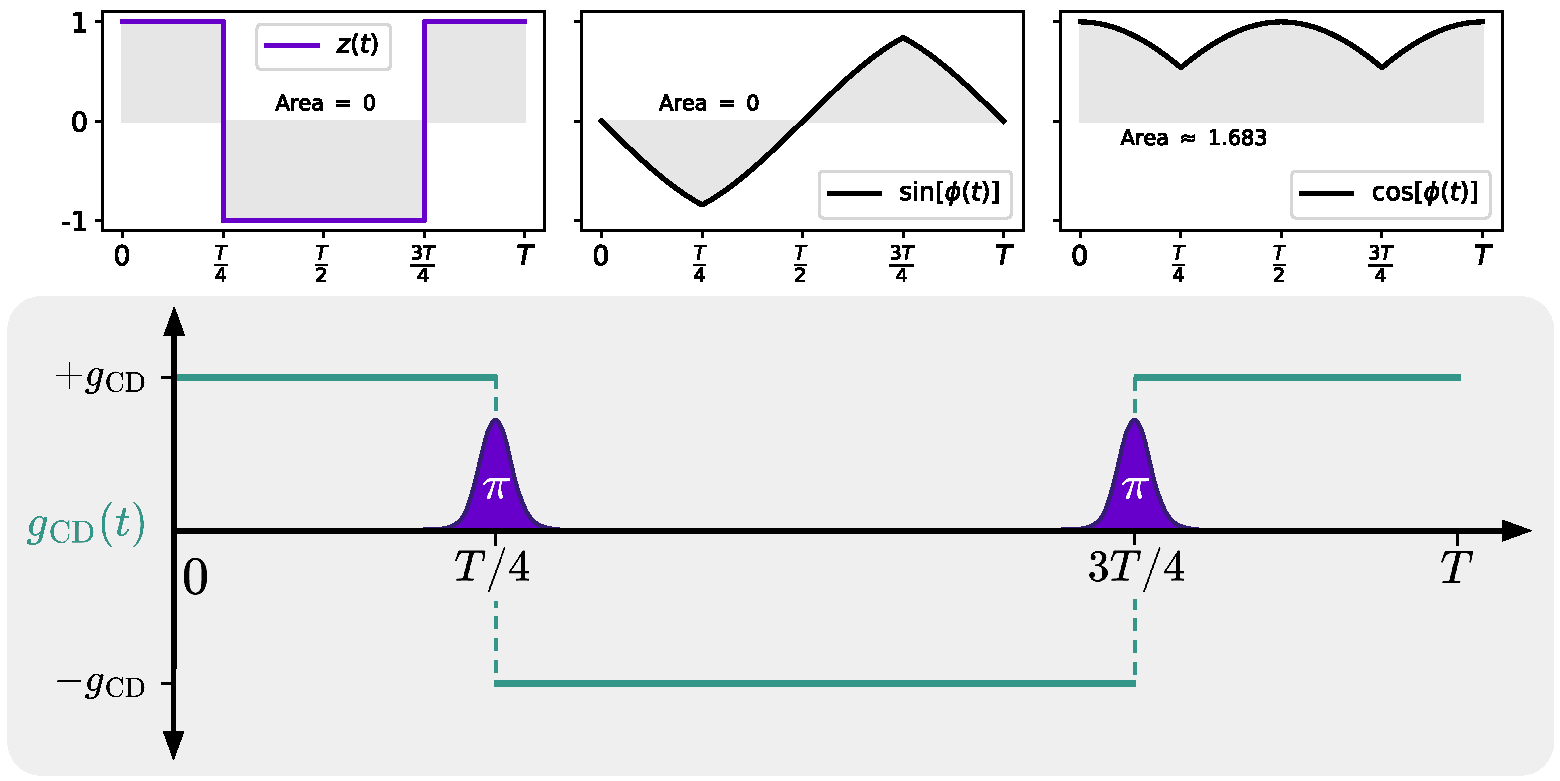
\includegraphics[width=\linewidth]{Figures/5/double_echo_FCD.pdf}
    \caption{FCD pulse implementation using the double-echo $\pi$-pulse schedule $z(t)$. Top row: numerical example of $z(t)$, $\sin[\phi(t)]$, and $\cos[\phi(t)]$ for $T = 2$ and $\chi = 4$. Observe $z(t)$ has an integral of zero as required. By modulating $g_{\rm CD}(t)$ to match the time-dependence of $z(t)$, we get constant $g_{\rm CD}(t)z(t) = 1$. The areas under $\sin[\phi(t)]$ and $\cos[\phi(t)]$ then give the relative magnitudes of the unconditional and conditional displacement rates in the FCD unitary. Bottom row: full ideal FCD pulse sequence showing the $\pi$-pulses and $g_{\rm CD}(t)$.}
    \label{fig:5_double_echo_FCD}
\end{figure}

We performed numerical simulations of the FCD gate using a two-level qubit truncated version of the full Hamiltonian in Eq. \eqref{eq:5_FCD_full_hamiltonian}, and found that the double $\pi$-pulse sequence we constructed indeed allows us to echo away the unwanted terms (such as the dispersive term $\chi_{aq}$, the displacement $g_{\rm disp}$, and the nonlinear displacement $g_a$). Unfortunately, however, we also find that the strength of the unconditional displacement $g_{\rm disp}$ in this scheme can be much larger than the conditional displacement $g_{\rm CD}$; using realistic device parameters we found that $g_{\rm disp}$ is often an order of magnitude larger. As a result, we expect that a separate ``cancellation drive'' on the storage will be required if we want to implement the FCD scheme in practice. 

Beyond this, we also found that the various design constraints for a realistic RAT device can be quite demanding, as it is somewhat difficult to hit the various couplings and mode capacitances during design/simulation. Moreover, the transmon control qubit in the RAT approach would still be susceptible to frequent bit-flip errors, limiting the GKP code performance. For these reasons, we chose to develop an alternative to the RAT with a fluxonium control qubit in place of the transmon; we will discuss this next. 

Despite the challenges associated with it, the RAT remains a novel and interesting theoretical proposal for implementing GKP error correction, and we hope the ideas behind it may be useful in developing further experiments in the future. 
 \clearpage
 %%%%%%%%%%%%%%%%%%%%%%%%

\section{The Resonator-ATS-Fluxonium (RAF) Experiment \label{sec:5_RAF}}

Our current main approach to realizing GKP error correction in 2D is called the RAF. It builds upon the idea of using an ATS as a coupler to realize fast conditional displacements, but instead uses a heavy fluxonium control qubit. To understand the principle behind the RAF, we start from the Hamiltonian for a coupled a storage resonator, ATS, and fluxonium system: $\hat{H} = \hat{H}_a + \hat{H}_b + \hat{H}_q + \hat{H}_{\rm int}$, where $\hat{H}_{\rm int}$ is a linear capacitive coupling term and $\hat{H}_q$ is:
\begin{equation}
    \hat{H}_q = 4E_C \hat{n}_q^2 + \frac{1}{2}\hat{\theta}^2 - E_J\cos(\hat{\theta}-\theta{\rm ext}) = \omega_{q, 0} \hat{q}_0^\dagger\hat{q}_0 - E_J\cos(\hat{\theta}-\theta{\rm ext})
\end{equation}
Here we have written the fluxonium Hamiltonian in its ``LC basis'' (i.e. the Fock basis for the linear part of the circuit). Following our approach in Sec. \ref{sec:5_RAT}, we can now analyze the full coupled system using a normal mode basis, i.e. absorbing the linear coupling term to get three normal modes $\hat{a}$, $\hat{b}$, and $\hat{q}$ for the storage, ATS, and qubit respectively. In this basis, 
\begin{equation}
    \hat{H} = \sum_{c = \{a, b, q\}}\omega_c \hat{c}^\dagger \hat{c} - E_{J,q}\cos(\hat{\theta}-\theta_\mathrm{ext}) - 2E_J \cos(\varphi_\Sigma)\cos(\hat{\varphi} + \varphi_\Delta)
    \label{eq:RAF_H}
\end{equation}
where the phase operators $\hat{\theta}$ and $\hat{\varphi}$ for the fluxonium and ATS may be expressed as linear combinations of $\hat{a}, \hat{a}^\dagger$, $\hat{b}, \hat{b}^\dagger$, and $\hat{q}, \hat{q}^\dagger$ as in Eq. \eqref{eq:linear_basis_RAT_RAF}, in terms of the participations $\theta_a, \theta_b, \theta_q$ ($\phi_a, \phi_b, \phi_q$) of the the various modes in the fluxonium (ATS) phase. This basis is reminiscent of black-box quantization, but we stress here that no approximation has been made --- as long as we do not truncate the fluxonium, Eq. \eqref{eq:RAF_H} is exact. 

To implement conditional displacements with the RAF, we bias the ATS at the \textit{symmetric} bias point $(\varphi_\Sigma, \varphi_\Delta) = (\pi/2, 0)$ and modulate about this via $\varphi_\Sigma(t) = \pi/2 + \epsilon(t)$. In this case, we get
\begin{equation}
    \hat{H} = \sum_{c = \{a, b, q\}}\omega_c \hat{c}^\dagger \hat{c} - E_{J,q}\cos(\hat{\theta}-\theta_\mathrm{ext}) - 2E_J \sin[\epsilon(t)]\cos\hat{\varphi}
    \label{eq:RAF_H_biaspoint}
\end{equation}
The fluxonium nonlinear term will now give rise to dispersive shifts $\chi_{xy}$ between the three modes, as well as Kerr nonlinearities $K_x$ for $x, y \in \{a, b, q\}$, while the ATS nonlinear term will give us the desired microwave-activated conditional displacement interaction. Let's now focus on the latter term. We can write $\hat{\varphi} = \hat{\varphi}_a + \hat{\varphi}_b + \hat{\varphi}_q$ and Taylor expand the drive $\sin[\epsilon(t)] \approx \epsilon(t) = \epsilon_p\cos(\omega_p t)$. Doing so, we can express this part of the Hamiltonian $\hat{H}_{\rm CD}$ as follows:
\begin{equation}
    \hat{H}_{\rm CD} = - 2E_J\epsilon(t)\big[\cos\hat{\varphi}_q\cos{(\hat{\varphi}_a + \hat{\varphi}_b)} - \sin\hat{\varphi}_q\sin{(\hat{\varphi}_a + \hat{\varphi}_b)}\big]
    \label{eq:RAF_HCD_expanded}
\end{equation}
Here, we have used a trigonometric identity to separate out the qubit ($\hat{\varphi}_q$) terms from the others, for the following reason. The storage $\hat{\varphi}_a = \varphi_a(\hat{a} + \hat{a}^\dagger)$ and ATS $\hat{\varphi}_b= \varphi_b(\hat{b} + \hat{b}^\dagger)$ both have small phase fluctuations, which will allow us to Taylor expand using $\varphi_a, \varphi_b$ as small parameters. Meanwhile, the fluxonium \textit{cannot} be expanded in this manner, and thus we must keep the full nonlinearities $\sin(\hat{\varphi}_q)$ and $\cos(\hat{\varphi}_q)$. Keeping this in mind, we can expand to 
\begin{equation*}
    \cos{(\hat{\varphi}_a + \hat{\varphi}_b)} = \cos\hat{\varphi}_a\cos \hat{\varphi}_b - \sin\hat{\varphi}_a\sin \hat{\varphi}_b \approx \bigg[1 - \frac{\hat{\varphi}_a^2}{2}\bigg]\bigg[1 - \frac{\hat{\varphi}_b^2}{2}\bigg] - \hat{\varphi}_a\hat{\varphi}_b
\end{equation*}
and 
\begin{equation*}
    \sin{(\hat{\varphi}_a + \hat{\varphi}_b)} = \sin\hat{\varphi}_a\cos \hat{\varphi}_b + \cos\hat{\varphi}_a\sin \hat{\varphi}_b \approx \hat{\varphi}_a\bigg[1 - \frac{\hat{\varphi}_b^2}{2}\bigg] + \hat{\varphi}_b\bigg[1 - \frac{\hat{\varphi}_a^2}{2}\bigg]
\end{equation*}
If we now go into the rotating frames of modes $a$ and $b$, and further set the ATS flux drive frequency to the storage frequency $\omega_p = \omega_a$, then we can perform an RWA on Eq. \eqref{eq:RAF_HCD_expanded} to get an effective
\begin{equation}
    \hat{H}_{\rm CD} = 2E_J \bigg[1 - \frac{\varphi_b^2}{2} - \varphi_b^2\hat{b}^\dagger\hat{b}\bigg]\bigg(\frac{\epsilon_p}{2}\bigg)\hat{\varphi_a}\sin(\hat{\varphi}_q)
\end{equation}
Finally, assuming that the ATS mode is never populated due to its detuning from the other modes, we set $\ev{\hat{b}^\dagger\hat{b}} \approx 0$ and can then expand $\hat{\varphi}_a = \varphi_a(\hat{a} + \hat{a}^\dagger)$ to get a final effective Hamiltonian
\begin{equation}
    \hat{H}_{\rm CD} = E_J  \epsilon_p\varphi_a \bigg[1 - \frac{\varphi_b^2}{2} \bigg](\hat{a} + \hat{a}^\dagger)\sin\hat{\varphi}_q \triangleq \hat{H}_{\rm CD}^{(q)} (\hat{a} + \hat{a}^\dagger)
\end{equation}
where we group the prefactors and qubit terms into $\hat{H}_{\rm CD}^{(q)}$. From here, we can calculate the displacement and conditional displacement rates via the sum and difference matrix elements of the qubit part:
\begin{align}
    \begin{split}
        g_\mathrm{disp} &= \frac{1}{2}\Big[\langle g|\hat{H}_{\rm CD}^{(q)}|g\rangle + \langle e|\hat{H}_{\rm CD}^{(q)}|e\rangle \Big] = A\bigg[\langle g|\sin\hat{\varphi}_q|g\rangle + \langle e|\sin\hat{\varphi}_q|e\rangle\bigg] \\
        g_{\rm CD} &= \frac{1}{2}\Big[\langle g|\hat{H}_{\rm CD}^{(q)}|g\rangle - \langle e|\hat{H}_{\rm CD}^{(q)}|e\rangle \Big] = A\bigg[\langle g|\sin\hat{\varphi}_q|g\rangle - \langle e|\sin\hat{\varphi}_q|e\rangle\bigg]
    \end{split}
\end{align}
with a common scale factor $A = \frac{1}{2}E_J\epsilon_p   \varphi_a[1 - \varphi_b^2/2]$. If we truncate the qubit to a two-level subspace, we get
\begin{equation}
    \hat{H}_{\rm CD}^{\rm tls} = g_{\rm disp} (\hat{a}+\hat{a}^\dagger) + g_{\rm CD} (\hat{a}+\hat{a}^\dagger)\hat{\sigma}_z
\end{equation}
This is precisely the conditional displacement interaction we wanted, though it also comes with an additional direct displacement. It so happens, however, that for a heavy-fluxonium away from half-flux, the difference in matrix elements (i.e. $g_{\rm CD}$) can be quite large, while the sum (i.e. $g_{\rm disp}$) can be made quite small; nonetheless, we envision using a cancellation drive to null out the displacement. 

In practice, starting from Eq. \eqref{eq:RAF_H_biaspoint}, we diagonalize the qubit Hamiltonian numerically to compute \textit{all} metrics of interest, such as dispersive shifts and Kerr nonlinearities, in terms of the relevant fluxonium matrix elements. Going from this theoretical proposal to a fully realized experiment took many rounds of design, simulation, and refinement of the theory before we arrived at a final parameter set for the system that satisfied all of the experimental design constraints. I will not discuss these details here; for a more complete treatment, I direct readers to the SM thesis of my colleague Shantanu Jha. 

Instead, I will here just briefly summarize the main results. For our final choice of system parameters, we are able to achieve a large conditional displacement rate $g_{\rm CD}/2\pi \simeq 4$ MHz over a wide range of qubit external flux bias points as shown in Fig. \ref{fig:5_RAF_Metrics}. Over this range, the dispersive shift $\chi_{aq}$ between the fluxonium and storage remains small, and so we don't expect to be limited by oscillator dephasing during qubit reset (which, as we recall from Ch. \ref{ch:4_3DGKP}, was an important consideration in our 3D dispersive experiment and the reason we engineered a flux-tunable dispersive shift to cross through zero there). Lastly, the Kerr nonlinearities $K_g$ and $K_e$ inherited by the storage resonator are neglible (mHz-level). With these values, we expect to be able to achieve state-of-the-art GKP QEC performance. In Fig. \ref{fig:5_RAF_Final_Design}, I also show a false-color image of the final design for the RAF, which is being fabricated as of this writing. In addition the core storage, ATS, and fluxonium subsystem, we have also incorporated a readout resonator and Purcell filter to be able to achieve faster unconditional qubit reset in approximately 100 ns via fluxonium sideband cooling. With this, we expect to be able to perform a cycle of SBS error correction within $\delta t = 400$ ns. 

\begin{figure}[h]
    \centering
    \includegraphics[width=0.95\linewidth]{Figures/5/RAF_Metrics.pdf}
    \caption{Simulated metrics of interest for the RAF using our final design parameters. We get a CD rate of $g_{\rm CD}/2\pi \simeq 4$ MHz across a wide band of external flux operating points $\theta_{\rm ext}$ for the qubit, as well as low residual dispersive shift $\chi_{aq}$ to the storage ($< 0.5$ kHz) and negligible (mHz-level) Kerr nonlinearity.}
    \label{fig:5_RAF_Metrics}
\end{figure}

\begin{figure}[h]
    \centering
    \includegraphics[width=0.7\linewidth]{Figures/5/RAF_Final_Design.pdf}
    \caption{Final chip design for the RAF, consisting of a storage resonator, ATS coupler, and fluxonium control qubit, as well as a readout resonator and Purcell filter for fast reset. For more details, we invite readers to refer to the upcoming SM thesis of Shantanu Jha.}
    \label{fig:5_RAF_Final_Design}
\end{figure}

\clearpage


\section{The 2D Dispersive Experiment: Moving 3D \texorpdfstring{$\to$}{to} 2D\label{sec:5_2D_Disp}}

Our final proposed approach to implement GKP error correction in 2D is our so-called 2D dispersive project. We came up with this approach during the penultimate stage of design for the RAF, which also coincided with our last attempts to fix the storage coherence issues in our 3D dispersive experiment (these issues turned out to be inherent to our 3D package). Given the daunting possibility of having to redesign the 3D experiment from scratch this late into the project, we set out to identify as many alternative paths forward as possible and ultimately settled on the following: why not move the dispersive coupling experiment entirely to 2D, replacing the 3D cavity with an on-chip resonator? This idea was attractive to us for several key reasons: 
\begin{enumerate}
    \item In 2D, the storage and fluxonium can be directly coupled capacitively and we don't need an antenna to mediate the coupling. By reducing one linear mode, this would help alleviate the parasitic Purcell resonances that we saw in  Sec. \ref{sec:4_fluxonium_T1}.
    \item In contrast to 3D, fast-flux control of the qubit can be implemented straightforwardly via on-chip flux lines in 2D. 
    \item Specific to our fabrication workflow in EQuS, a 2D design could be fabricated using a standard 2" wafer at Lincoln Lab as opposed to the 8" wafer that was required for the fluxonium chips we used in our 3D experiment; using the more standard process would help with fabrication time, yield, and parameter targeting. 
    \item We could use the design/simulation infrastructure already developed for the RAF to expedite the process. Indeed, this ultimately proved to be the single most important factor and enabled us to go from ideation to a complete design in under two months. 
    \item It is a simpler 2D experiment than the RAF, and so helps mitigate the risk of failure. 
\end{enumerate}

Of course, as we noted in the previous section, 2D resonators have higher single-photon losses. A 2D dispersive design relying on ECD would not be able to correct such errors as efficiently as the RAF. Nonetheless, given our strategy of using a large gap low-frequency resonator, it seems within the realm of possibility to achieve a storage resonator lifetime of $T_1 \simeq 100$ $\mu$s. As we will see below, this would already be enough to demonstrate QEC. 

\subsection{System Parameters and Design Overview}
The 2D dispersive design consists of four main elements: the storage resonator, fluxonium qubit, readout resonator, and a Purcell filter to help achieve larger resonator linewidth for the SBS reset without causing excess loss to the qubit. As with the RAF, the various design parameters here were chosen to balance many different experimental constraints, and had to be iteratively refined via successive rounds of simulation. The final design is shown in Fig. 5-1, and we will now discuss some of the design considerations that went into it.
\begin{figure}[h] 
    \begin{subfigure}{\linewidth}
        \centering
        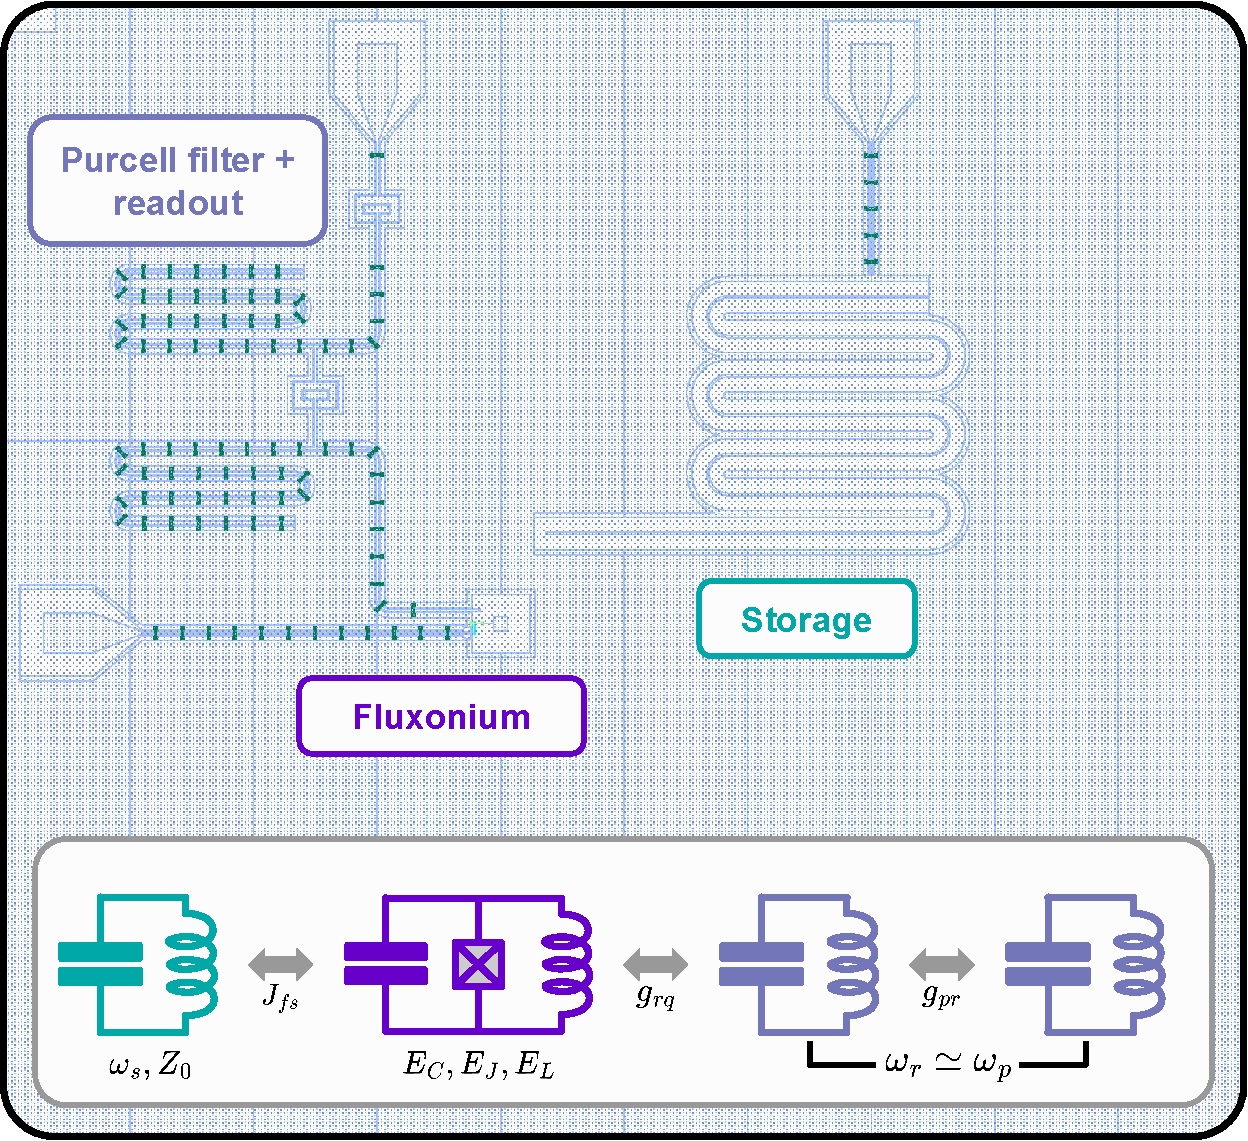
\includegraphics[width=0.8\linewidth]{Figures/5/2D_Dispersive_GDS.pdf}
        \vspace*{2mm}
    \end{subfigure} 
    \begin{subfigure}{\linewidth}
        \centering
        \begin{tabular}{c|c|c|c|c|c|c|c|c }
       $\omega_s/2\pi$ & $J_{fs}/2\pi$ & $E_J/h$  & $E_C/h$ & $E_L/h$ & $g_{rq}/2\pi$ & $\omega_r/2\pi$ & $\omega_p/2\pi$ & $g_{pr}/2\pi$\\\hline
        4134.0 & 3.0 & 3754.9 & 844.0 & 299.9 & 42.1 & 6125.0 & 6137.0 & 27.6
    \end{tabular}
    \end{subfigure}
    \caption{Final GDS design and parameters for the 2D dispersive experiment, showing the on-chip storage resonator, fluxonium qubit, readout resonator, and Purcell filter. The frequency parameters for the various elements in the table are all listed in MHz}
    \label{fig:5_2D_Dispersive_GDS}
\end{figure}

\noindent \textbf{Fluxonium:} We chose the nominal qubit parameters $E_J, E_C, E_L$ shown above in Fig. \ref{fig:5_2D_Dispersive_GDS} to achieve a moderately heavy fluxonium with a frequency of $\omega_q/2\pi \simeq 107$ MHz at half-flux. We expect this will result in a long $T_1^{g\to e}$ away from the sweet spot. These parameters also ensured that the qubit plasmon transition frequencies were high enough to not be limited by heating out of the $\ket{g}$-$\ket{e}$ manifold. 


\noindent \textbf{Storage and Fluxonium System:} The storage mode was designed as a large gap (60 $\mu$m) $\lambda/4$ coplanar waveguide resonator with a resulting impedance of $Z_0 = 95.127$ $\Omega$. We chose its frequency to be as low as possible to maximize $T_1$ given a constant $Q = \omega_s T_1$, ultimately settling on $\omega_s/2\pi = 4.134$ GHz. This was co-designed with the fluxonium so as to achieve bosonic mode threading. For the fluxonium-storage coupling $J_{fs}$, we performed numerical diagonalization simulations of the following Hamiltonian (similar to that in Ch. \ref{sec:4_3D_Experiment_Design_Theory}):
\begin{equation}
    \hat{H} =  \hat{H}_s + \hat{H}_{\rm int} + \hat{H}_{\rm fluxonium} =  \omega_s \hat{a}^\dagger \hat{a} + J_{fs} \hat{n}\hat{n}_a + \Big[4E_C \hat{n}^2 + \frac{1}{2}\hat{\varphi}^2 - E_J\cos(\hat{\varphi}-\varphi_{\rm ext})\Big],
\end{equation}
using which we calculated the dispersive shift $\chi = \omega_s^{|e\rangle} - \omega_s^{|g\rangle} = [E_{e,1} - E_{e, 0}] - [E_{g, 1} - E_{g, 0}]$ as well as the storage Kerr nonlinearities $K = (K_g + K_e)/2$ and $dK = (K_g - K_e)/2$ defined by $K_{g/e} = E_{g/e, 2} + E_{g/e, 0} - 2E_{g/e, 1}$. We then manually varied $\omega_s$ and $J_{fs}$ so as to achieve a low $K$ and $dK$ (on the order of Hz)\footnote{We have seen in simulations that the average Kerr $K$ is worse for GKP performance than differential Kerr $dK$. We can typically afford $dK$ to be slightly (as much as 5-10x) larger than $K$; ideally we have $K < 5$ Hz.} over the external flux range of interest $\Phi_{\rm ext}/\Phi_0 \in [0.42, 0.5]$, while also having a flux-tunable $\chi$ that crosses through zero and that is large enough away from this zero-crossing to perform ECD. We tried to target similar values for $\chi$, $K$, and $dK$ as Ref. \cite{sivak2023gkp-expt}, and ultimately chose the operating point $\Phi_{\rm ext} \simeq 0.43\Phi_0$ where $\chi/2\pi \simeq 50$ kHz, $K/2\pi \simeq 1$ Hz, and $dK/2\pi \simeq 10$ Hz, as shown in Fig. \ref{fig:5_2D_dispersive_metrics}(c). Meanwhile, the reset point at which the storage dispersive shift $\chi \to 0$ occurs at $\Phi_{\rm ext} \simeq 0.475\Phi_0$. 
\begin{figure}[h]
    \centering
    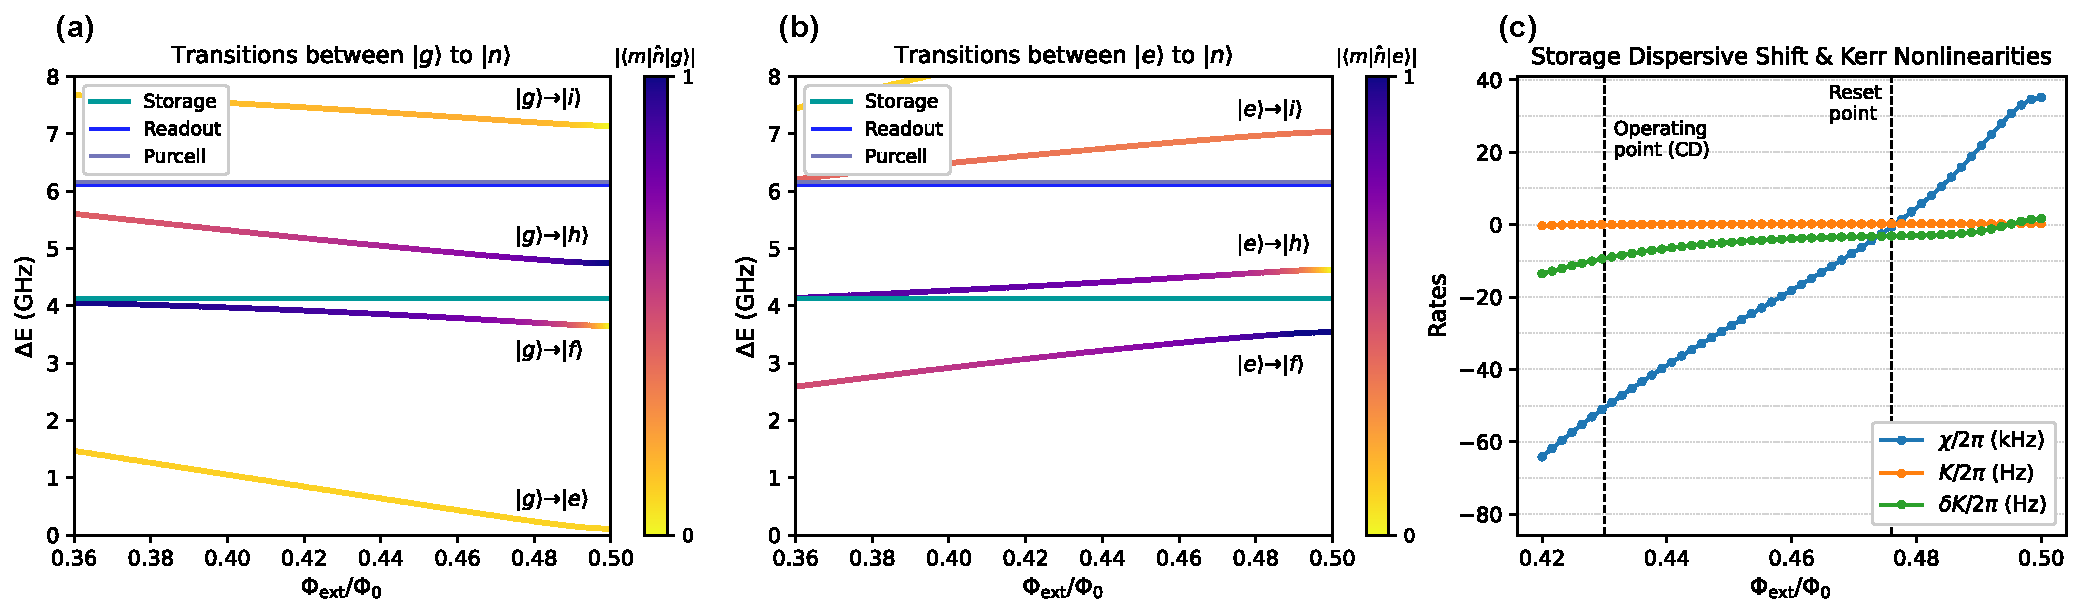
\includegraphics[width=\linewidth]{Figures/5/2D_dispersive_metrics.pdf}
    \caption{\textbf{(a, b)} Simulated fluxonium spectrum for 2D dispersive experiment showing transitions $\ket{g/e}\to\ket{n}$ and the associated charge matrix elements. The storage mode (teal) is threaded between the two sets of plasmon transitions. \textbf{(c)} Simulated storage dispersive shift $\chi$ (kHz), average Kerr $K$ (Hz) and differential Kerr $dK$ (Hz). We label the operating points where we perform reset and conditional displacements (CD) respectively.}
    \label{fig:5_2D_dispersive_metrics}
\end{figure}

\noindent \textbf{Readout and Purcell Filter:} We used a similar design for the readout resonator and Purcell filter as the RAF; both resonators were standard 50 $\Omega$ coplanar waveguide resonators with frequencies $\omega_r/2\pi = 6.125$ and $\omega_p/2\pi = 6.137$. We chose $g_{pr}$ to be greater than the detuning of the modes, so that the two are almost fully hybridized with normal mode frequencies of roughly $\omega_r - g_{pr}$ and $\omega_p + g_{pr}$ [to see this, diagonalize $\hat{H}_{pr} = \omega_r\hat{r}^\dagger \hat{r} + \omega_p\hat{p}^\dagger \hat{p} + g_{pr}(\hat{r}^\dagger\hat{p} + \hat{r}\hat{p}^\dagger)$]. The Purcell filter is strongly coupled to a transmission line with a coupling of $\kappa_p/2\pi \simeq 38.8$ MHz. By choosing $g_{pr} \lesssim \kappa_p$, this results in an effective readout coupling rate of $\kappa_r/2\pi \simeq 16$ MHz. The reason for choosing such a large value of $\kappa_r$ is to implement fast unconditional reset of the qubit. As shown in Fig. \ref{fig:5_SBS_Sideband_Reset}, our proposed approach to implement the reset is via direct fluxonium sideband cooling, as was recently demonstrated in Ref. \cite{najera2024high}. This is done by driving the $\ket{e0}\leftrightarrow\ket{g1}$ transition between the qubit and resonator away from the half-flux sweet spot; the strong loss on the resonator will then cause this to decay to $\ket{g0}$. In this manner, we can realize fast unconditional reset of the fluxonium, as is required for the SBS protocol.

\begin{figure}[h]
    \centering
 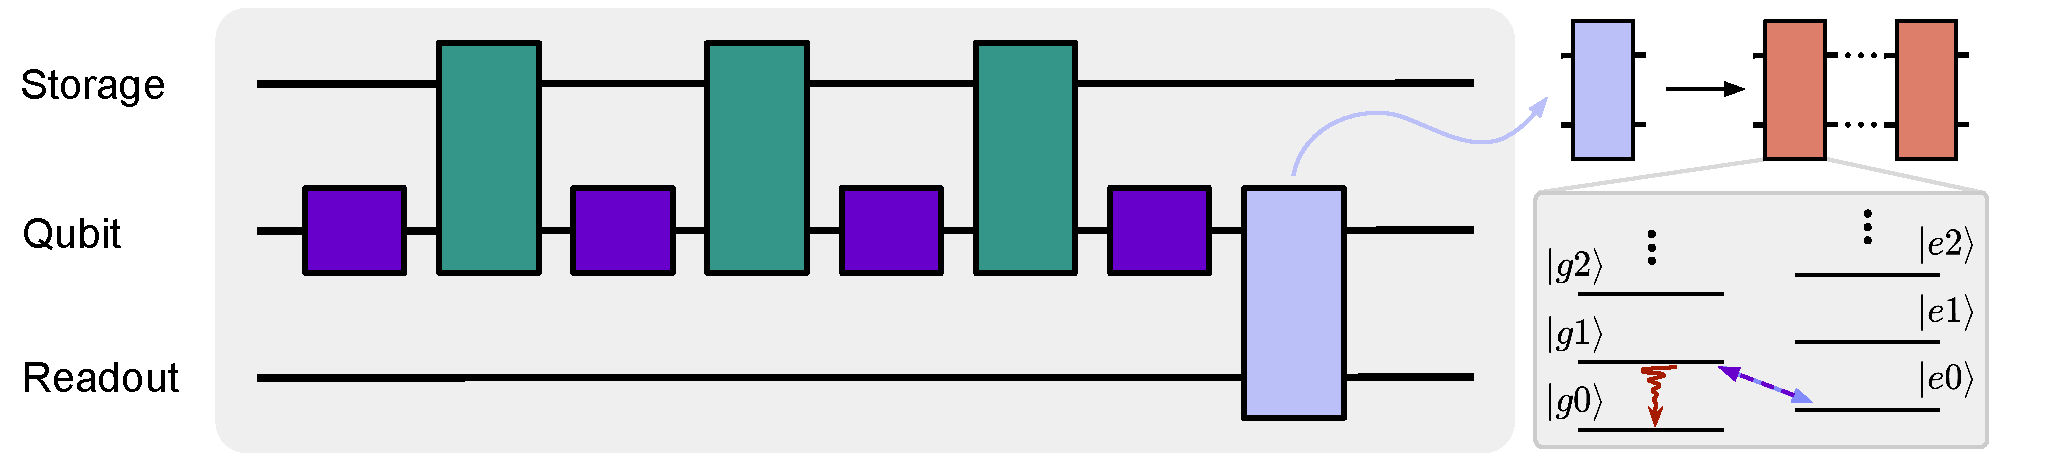
\includegraphics[width=\linewidth]{Figures/5/SBS_Sideband_Reset.pdf}
    \caption{SBS sequence consisting of 3 conditional displacements (teal), 4 qubit pulses (purple),  and unconditional qubit reset (lilac). The reset can be further decomposed into a number of dissipative swap operations based on fluxonium $\ket{e0}\leftrightarrow\ket{g1}$ sideband cooling.}
    \label{fig:5_SBS_Sideband_Reset}
\end{figure}

\clearpage
\subsection{Performance Estimates}

The first check we carried out when assessing the feasibility of a 2D dispersive design was to determine how quickly we can implement a round of SBS (i.e. one quadrature of QEC). We based this on preliminary simulations from our theory collaborators Jonathan Pelletier and Baptiste Royer that indicated\footnote{These simulations aren't yet published, but they show that the maximum storage photon number at which ECD starts to break in simulation is similar or even slightly higher for a fluxonium than for a transmon.} that a fluxonium qubit is not significantly different than a transmon from the perspective of carrying out ECD. As a result (cf. above), we designed our storage-fluxonium system to have a similar dispersive shift and Kerr nonlinearity as the storage-transmon system from Ref. \cite{sivak2023gkp-expt}, and assumed in what follows that we can use a similar photon number (approximately 100-140 storage photons) in ECD. 

\noindent The sequence for SBS is shown in Fig. \ref{fig:5_SBS_Sideband_Reset}: it consists of 4 conditional displacements (CDs), 3 qubit $\pi/2$ rotations, and qubit reset. We assume our CDs take the same time as Ref. \cite{sivak2023gkp-expt} and that our qubit pulses each take 32 ns; meanwhile for reset, we follow Ref. \cite{nordquantique2023gkp-expt} where the authors used $N_{\rm reset} = 2$ dissipative swaps. In our case, our readout has a linewidth of $\kappa_r / 2\pi \approx 16$ MHz, giving a $T_1 \simeq 9$ ns. From here, we estimate our worst case reset time to be $T_{\rm diss. swap} \simeq 132$ ns\footnote{This estimate is based on comparing to the parameters of Ref. \cite{nordquantique2023gkp-expt}; we hope it will be a worst-case value}. In total, the time $\delta t$ that we estimate it will take for an SBS round is:
\begin{align*}
\delta t = T_{\rm sBs}  &= 4T_{\rm pi} + (T_{\rm CD\,1} + T_{\rm CD\,2} + T_{\rm CD\,3}) + \big[N_{\text{reset}}\times T_{\text{diss. swap}}\big] \\ &= 4\times (32) + (470 + 676 + 230) + \Big[2 \times 132\Big] = 1768\, {\rm ns}
\end{align*}
We performed extensive SBS simulations using this value of $\delta t$, assuming different levels of single-photon loss $\kappa_{1s}$. We followed the method from Sec. \ref{sec:2_simulations_SBS} by modelling the sequence as an instantaneous QEC channel followed by a loss channel of length $\delta t$ (recall, this gives a lower bound on logical lifetime). For the QEC, we additionally optimized over the error correction parameters (i.e. code size $\Delta$ and small displacements $\epsilon_1, \epsilon_2$) to find the highest logical lifetime $T_L$ at each value of $T_{1s} = 1/\kappa_{1s}$. The results are shown in Fig. \ref{fig:2D_vs_3D_SBS_Comparison}; we plot the dimensionless quantity $T_L/\delta t$ (the number of rounds we can stabilize for) vs. $T_{1s}/\delta t$, the effective storage lifetime in units of the SBS cycle time. We repeat this process for the three cases: (i) a perfect/lossless control qubit (blue); (ii) a control qubit with $T_1 = 1.2$ ms (orange); and (iii) a control qubit with $T_1 = 300$ $\mu$s (green). For each value of $T_{1s}$ we also plot the lifetime of the oscillator $\{\ket{0}, \ket{1}\}$ Fock qubit (black), which is calculated as done in Ref. \cite{royer2020gkp} by $T_L^{\rm fock} = T_{1s}/2$. We see from these results that, at least in simulation, we are able to achieve break-even over the oscillator Fock encoding in all cases. 

\begin{figure}[t]
    \centering
    \includegraphics[width=0.8\linewidth]{Figures/5/2D_vs_3D_SBS_Comparison.png}
    \caption{Simulated plot of dimensionless maximum GKP logical lifetime $T_L/\delta t$ from SBS simulations vs. dimensionless storage lifetime $T_{1s}/\delta t$. Here $\delta t$ is the SBS cycle time. We optimized over GKP code parameters to find the maximum $T_L$ at each value of $T_{1s}$, and repeat this for the cases of a lossless qubit, a qubit with $T_1 = 1.2$ ms (e.g. a fluxonium), and a qubit with $T_1 = 300$ $\mu$s (e.g. a transmon). We find that all three cases outperform the bare oscillator Fock encoding here. The ranges in grey are overlaid on the plot assuming $\delta t = 1.7$ $\mu$s and $T_{1s} \in [45, 200]$ $\mu$s for the 2D dispersive experiment; $\delta t = 2.8$ $\mu$s and $T_{1s} \in [200, 700]$ $\mu$s for the 3D dispersive experiment; and finally $\delta t = 400$ ns and $T_{1s} \in [45, 200]$ $\mu$s for the 2D parametric experiment (RAF).}
    \label{fig:2D_vs_3D_SBS_Comparison}
\end{figure}

\noindent Of course, in practice, the logical lifetime will be reduced by many other experimental factors. But, we see from this that it is at least plausible to realize break-even error correction. Finally, since these curves depend only on the product $\kappa_{1s}\delta t$ (i.e. on $T_{1s}/\delta t$), we can use the x-axis to get a sense of the required storage lifetimes for each of our three experiments: the 3D dispersive, the 2D dispersive, and the RAF (2D parametric). We overlay the three expected performance ranges on the plot; what we see is that in the best case scenario, the performance of the 2D dispersive experiment should not be too far behind the ideal performance that we had originally hoped for in our 3D experiment. Additionally, by the same metric, we see that the RAF experiment has the potential to far outperform the other two approaches, and so we expect to be able to achieve state-of-the-art QEC gain here.

Overall, we find that both of our upcoming experiments represent promising pathways towards realizing robust and extensible GKP error correction in 2D. The expect to receive both the RAF and 2D dispersive designs shortly after this writing, and are excited to test these platforms in experiment.  



\printbibliography[heading=subbibliography, title = References]
\printbibliography[heading=subbibliography, title = References]
\clearpage
% % ------------------------------------------------

%%%%% Appendix A: Resonator Fitting %%%%%%
\appendix
\chapter{Appendix: Resonator Fitting\label{ch:AppA}}

A large part of the experimental work done in this thesis involves probing 3D cavity resonators using classical microwave fields. In doing so, we are able to infer various properties of the resonator such as its internal and coupling losses. In this appendix, we derive from first principles the resonance lineshape of a single-mode resonator coupled a readout transmission line. This simple example can be treated theoretically using the \textit{input-output formalism}, yet it is general enough to cover several of the experiments performed in this thesis. In order to bridge the gap between this model and our experimental setup, we also extend our analysis to the include (a) reflection measurements using a circulator, (b) asymmetric lineshapes due to so-called Fano resonances, and (c) the calculation of transmission coefficients when the mode is connected to separate transmission lines. 

\section{Input-Output Theory for Resonators}
\subsection{Single-Mode Reflection Measurements}

Let's consider a linear resonator mode $\hat{a}$ with angular frequency $\omega_0$ coupled to a transmission line. The Hamiltonian describing this mode is that of a quantum harmonic oscillator, $\hat{H} = \myhbar\omega_0 \hat{a}^\dagger \hat{a}$. Without the transmission line, the dynamics of $\hat{a}$ are given in the Heisenberg picture by $\partial_t\hat{a} = -i[\hat{a}, \hat{H}] = -i\omega_0\hat{a}$, which leads to the familiar oscillatory motion of $\hat{a}(t)$ in phase space. However, if we include losses and coupling to the transmission line, the dynamics are modified in the form of a Heisenberg-Langevin equation \cite{walls1994quantum, gardiner2004quantum, clerk2010introduction}:
\begin{equation}
    \odv*{\hat{a}}{t}(t) = -i\omega_0\hat{a} - \Big(\frac{\kappa_c + \kappa_i}{2}\Big)\hat{a} + \sqrt{\kappa_c}\hat{a}_{\rm in}(t)
    \label{eq:A_heisenberg}
\end{equation}
Here, we include a damping term proportional to the total loss rate $\kappa = \kappa_c + \kappa_i$, where $\kappa_i$ is the \textit{intrinsic loss} of the mode due to uncontrolled interaction with environmental degrees of freedom and $\kappa_c$ is the \textit{coupling loss} to the transmission line (which we as experimenters may control for in design)\footnote{For a full derivation of this Heisenberg-Langevin equation in the context of superconducting circuits, two great expository references are the PhD theses of Audrey Bienfait \cite{bienfait2016thesis} and Steven Touzard \cite{touzard2019thesis}.}. The propagating fields inside  the transmission line are given by $\hat{a}_{\rm out}$ and $\hat{a}_{\rm in}$, as shown in Fig. \ref{fig:A_InputOutput}, with the latter giving rise to the source term $\sqrt{\kappa_c}\hat{a}_{\rm in}(t)$ in Eq. \eqref{eq:A_heisenberg}. At this point, let's also stop to introduce some useful terminology. If $\kappa_i < \kappa_c$, we refer to the resonator as \textit{overcoupled} and if $\kappa_i > \kappa_c$, we call it \textit{undercoupled}. Finally, if $\kappa_i = \kappa_c$, then the resonator is called \textit{critically coupled}. We will elaborate on the distinction between these cases later in this section. 


\begin{figure}[h]
    \centering
    \includegraphics[width=0.8\linewidth]{Figures/A/InputOutput.pdf}
    \caption{\textbf{(a)} Resonator mode $\hat{a}$ coupled to a transmission line is modeled via Eq. \eqref{eq:A_heisenberg}. \textbf{(b)} This setup can be realized using the electric field of a 3D superconducting post cavity.}
    \label{fig:A_InputOutput}
\end{figure}

\noindent In circuit QED experiments, we typically interact with readout resonators using a classical field $\alpha_{\rm in}(t)$ associated with a coherent state $\ket{\alpha_{\rm in}}$ in the input transmission line. Taking the expectation value on both sides of Eq. \eqref{eq:A_heisenberg}, we get $\partial_t \hat{a}(t) = -i\omega_0\hat{a} - (\kappa_c + \kappa_i)\hat{a}/2 + \sqrt{\kappa_c}\alpha_{\rm in}(t)$. Note that by defining the drive amplitude $\epsilon(t) = i\sqrt{\kappa_c}\alpha_{\rm in}(t)$, we can now self-consistently interpret the source term as coming from a Hamiltonian drive $\epsilon(t)(\hat{a} + \hat{a}^\dagger)$ on the system. 

If we examine the mean-value intra-resonator field $\alpha(t) = \ev{\hat{a}}(t)$ and take the Fourier transform $\mathcal{F}[\bullet]$ on both sides of the resulting equation, we can calculate\footnote{Recalling the definition $\mathcal{F}[\alpha(t)] \equiv \int \alpha(t) e^{i\omega t}dt$, we can derive $\mathcal{F}[\partial_t\alpha(t)] = -i\omega \alpha(\omega)$ via integration by parts.} the frequency domain response:
\begin{equation}
    \alpha(\omega) = \frac{2\sqrt{\kappa_c}}{\kappa_c + \kappa_i - 2i(\omega-\omega_0)} \alpha_{\rm in}(\omega)
    \label{eq:inputoutput-freq-domain}
\end{equation}
This equation gives us the ability to calibrate the mean circulating photon number $\bar{n} = |\alpha|^2$ in the resonator, in terms of the input power $P_{\rm in} = \myhbar\omega |\alpha_{\rm in}|^2$ seen by the device. Specifically, on resonance ($\omega = \omega_0$), we get:
\begin{equation}
    \bar{n} = \frac{4\kappa_c P_{\rm in}}{\myhbar\omega_0(\kappa_c + \kappa_i)^2}
\end{equation}
For overcoupled readout resonators with $\kappa_i \ll \kappa_c$, this reduces to $P_{\rm in} = \kappa_c\myhbar\omega_0 \bar{n}/4$. 

\noindent Now, the classical continuity equation for the propagating fields gives rise to the so-called \textit{input-output relation} \cite{clerk2010introduction}, which expresses the resonator mode $\hat{a}$ in terms of the transmission line fields: 
\begin{equation}
    \hat{a}_{\rm in}(t) + \hat{a}_{\rm out}(t) = \sqrt{\kappa_c} \hat{a}(t)
    \label{eq:inputoutput}
\end{equation}
In combination with Eq. \eqref{eq:inputoutput-freq-domain}, this relation allows us to express the reflected coherent output signal $\alpha_{\rm out}(\omega)$ in terms of the input signal $\alpha_{\rm in}(\omega)$ sent in to the resonator. In particular, their ratio defines
\begin{equation}
   S_{11}(\omega) = \frac{\alpha_{\rm out}(\omega)}{\alpha_{\rm in}(\omega)} = \frac{\kappa_c - \kappa_i + 2i(\omega - \omega_0)}{\kappa_c + \kappa_i - 2i(\omega - \omega_0)},
\end{equation}
i.e. a reflection coefficient. The choice to call this coefficient $S_{11}$ can be traced back to the S-matrix formalism \cite{kurokawa1965power, gardiner1985input}, which extends the analysis here to multi-port devices, and defines $S_{ij}(\omega) = \alpha_{{\rm out}, i}(\omega)/\alpha_{{\rm in}, j}(\omega)$. In this case, we only have a single-port resonator, and the reflected signal is given by $S_{11}(\omega)$; this is also what we measure experimentally using a Vector Network Analyzer (VNA). 

\section{Experimental Considerations}

\subsection{Fitting the Background}
Low order polynomial fits etc.

\subsection{Fano Resonance: Asymmetry in the Lineshape}
Modify the fit function to 
\printbibliography[heading=subbibliography, title = References]
\clearpage
% ------------------------------------------------

%%%%% Appendix B: Making 3D Cavities %%%%%%
\chapter{Appendix: Fabricating High-Q 3D Cavities \label{ch:AppB}}

In this brief appendix, we will review the standard operating procedures that we followed when fabricating aluminium 3D cavity resonators. Our overall procedure was developed through several iterations of cavities and so the version we present here is the final process that we eventually converged on. All of the 3D cavities used in this thesis were machined out of high-purity bulk aluminium with a grade of 5N5 (99.9995\% purity), as is typical for Al post cavity designs in past circuit QED experiments \cite{reagor2013reaching}. After designing and simulating the cavity, we submitted our specifications to the MIT Central Machine Shop for the actual machining of the device. Once we received the final machined cavities, the next steps were cleaning and etching; we performed both of these in the MIT.nano cleanroom.

For cleaning, we first dipped the cavity into a beaker of 1-methyl-2-pyrrolidone (NMP) for approximately a minute, until the color of the NMP changed to brown (removing any dirt or oils on the cavity left over from machining). We then did a more thorough cleaning by sequential sonication of the sample in (fresh) NMP, then acetone, and finally isopropyl alcohol (IPA). The solvents are chosen in the typical order of decreasing `strength' in order to remove machine oils and residues. We sonicate at a medium setting for 5 minutes each, transferring quickly between beakers to prevent solvent residues forming in air. After the IPA, we finally blow dry the sample with $N_2$ gas. 

Once the cavity is clean, we next proceed with the critical step of chemical etching in acid. The purpose of the etch is to treat surface imperfections and roughness of the aluminium, and it is a crucial ingredient for achieving high quality factor 3D resonators. We etch using the commonly-available Transene Aluminium Etchant Type A, which is a mix of nitric and phosphoric acid. The acid is heated to 50$^\circ$C using a hot plate and is temperature-controlled via a PID loop and thermometer. In our case, we placed the cavity in a teflon basket before lowering it into the acid bath along with a magnetic stir bar. We etched for 4 hours in total but replaced the acid every 45 minutes to prevent saturation. In each segment, we see the color of the acid change as the reaction proceeds as well as bubbles forming. We found it to be important to reorient the cavity within the acid in each segment to allow the bubbles to rise to the surface (and not get trapped within the cavity or below it). In our experience, this led to the best and most uniform etches, which indeed we saw translated into higher resonator lifetimes ---  after our most successful etch, we were able to measure cavities with single-photon lifetimes above 3 ms. We owe a special thanks to Miuko Tanaka for etching the first batch of 3D cavities, as well as to Aranya Goswami for his help in optimizing our etch process.

Following the acid treatment, we rinse the cavity in DI water for 5 minutes or more and then blow dry with $N_2$ gas. At this point, the cavity should have high lustre and the grain boundaries of the aluminium should be clearly visible. We finally perform another round of sonication in acetone and IPA for 3 minutes each before finally blow drying in $N_2$ again\footnote{We note that this process is slightly different to that in Ref. \cite{reagor2013reaching}, where the authors rinsed cavities in methanol following the acid etch. We did not try this yet, but leave it as an avenue for future 3D cavities we make.}.


\printbibliography[heading=subbibliography, title = References]
\clearpage
% ------------------------------------------------


%%%%% The End %%%%%%
%\cleardoublepage
%\phantomsection
%\addcontentsline{toc}{chapter}{References}
\sloppy
\end{document}